\documentclass[letter,11pt]{article}
\usepackage{amsmath}
\usepackage{tikz}
\usepackage{graphicx}
\makeatletter
\def\maxwidth{\ifdim\Gin@nat@width>\linewidth\linewidth\else\Gin@nat@width\fi}
\def\maxheight{\ifdim\Gin@nat@height>\textheight\textheight\else\Gin@nat@height\fi}
\makeatother
\setkeys{Gin}{width=\maxwidth,height=\maxheight,keepaspectratio}
\usepackage[spanish,es-tabla]{babel}
%\usepackage{draftwatermark}
%\SetWatermarkText{Preliminar}
\usepackage{gensymb}
\usepackage{parskip}
\usepackage[hidelinks]{hyperref}
\urlstyle{same}
\usepackage{caption}
\captionsetup{justification=justified,format=plain,font=small,labelfont=bf,margin=50pt}
\captionsetup[table]{name=\textbf{Tabla},labelsep=period}
\captionsetup[figure]{name=\textbf{Figura},labelsep=period}
\usepackage{fancyhdr}
\pagestyle{fancy}
\fancyhf{}
\usepackage[top=1.3cm,bottom=1.3cm,left=2.5cm,right=2.5cm]{geometry}
\usepackage{helvet}
\renewcommand{\familydefault}{\sfdefault}
\usepackage{multirow}
\usepackage{ragged2e}
\newcommand{\sietepuntos}{\fontsize{7pt}{\baselineskip}\selectfont}
\newcommand{\cincopuntos}{\fontsize{6pt}{\baselineskip}\selectfont}
\newcommand{\ochopuntos}{\fontsize{8.8pt}{\baselineskip}\selectfont}
\newcommand{\nuevepuntos}{\fontsize{9.6pt}{\baselineskip}\selectfont}
\usepackage{color,colortbl}
\definecolor{Gray}{rgb}{0.801,0.801,0.801}
\definecolor{Gray1}{rgb}{0.790,0.790,0.790}
\definecolor{Gray2}{rgb}{0.830,0.830,0.830}
\definecolor{Gray3}{rgb}{0.870,0.870,0.870}
\definecolor{Gray4}{rgb}{0.910,0.910,0.910}
%\addtolength{\headheight}{8.5\baselineskip}
\setlength{\headheight}{70pt}
\setlength{\footskip}{35pt}%5
\setlength{\textheight}{638pt}%658
\fancyhead[CE,CO]{
\includegraphics[height=1.5cm]{logoifop.png}\\ \sietepuntos INSTITUTO DE FOMENTO PESQUERO / DIVISION INVESTIGACION PESQUERA}
\fancyheadoffset{0.01cm}
\renewcommand{\headrulewidth}{0.5pt}
\renewcommand{\footrulewidth}{0.5pt}
\fancyfoot[CO,CE]{\cincopuntos \vspace{-0.6cm} \thepage \\ \vspace{0.4cm} %-------------------------------------------------------------------------------\\
\vspace{-0.2cm} \cincopuntos CONVENIO DE DESEMPE\~{N}O 2021 IFOP/SUBSECRETAR\'IA DE ECONOM\'IA Y EMT \\ \vspace{-0.1cm} DOCUMENTO T\'ECNICO. ANCHOVETA Y SARDINA ESPA\~{N}OLA, REGI\'ON DE ARICA Y PARINACOTA A LA REGI\'ON DE ANTOFAGASTA, 2022}
\author{}
\date{\vspace{-2.5em}}

\begin{document}

\begin{titlepage}
\begin{tikzpicture}
\node[anchor=south west,inner sep=0] at (0,0) {
\includegraphics[height=22.3cm,width=22cm,viewport=29 26 148 274]{portada1.pdf}};
%\node[anchor=south west,inner sep=0] at (0,0) {
\includegraphics[height=22.3cm,width=22cm,viewport=70 74 318 698]{portada1.pdf}};
\node[text width=8cm] at (13.85,16.60) {\large \textbf{DOCUMENTO T\'ECNICO}};
\node[text width=8cm] at (14.37,16.13) {\ochopuntos Convenio de Desempe\~{n}o 2021};
\node[text width=8cm] at (10.58,15.46) {\nuevepuntos Estatus y posibilidades de explotaci\'on biol\'ogicamente};
\node[text width=8cm] at (11.62,15.08) {\nuevepuntos sustentables de anchoveta y sardina espa\~{n}ola,};
\node[text width=10cm] at (9.60,14.72) {\nuevepuntos Regi\'on de Arica y Parinacota a la Regi\'on de Antofagasta, a\~{n}o 2022};
\node[text width=10cm] at (11.66,14.00) {\footnotesize \textbf{SUBSECRETAR\'IA DE ECONOM\'IA Y EMT / Junio 2021}};
\end{tikzpicture}
\end{titlepage}

\begin{titlepage}
\begin{tikzpicture}
\node[anchor=south west,inner sep=0] at (0,0) {
\includegraphics[height=22.3cm,width=22cm,viewport=70 74 318 698]{portada2.pdf}};
\node[text width=8cm] at (15.05,17.85) {\large \textbf{DOCUMENTO T\'ECNICO}};
\node[text width=8cm] at (15.43,17.38) {\ochopuntos Convenio de Desempe\~{n}o 2021};
\node[text width=8cm] at (11.85,16.50) {\nuevepuntos Estatus y posibilidades de explotaci\'on biol\'ogicamente};
\node[text width=8cm] at (12.86,16.09) {\nuevepuntos sustentables de anchoveta y sardina espa\~{n}ola,};
\node[text width=10cm] at (10.85,15.72) {\nuevepuntos Regi\'on de Arica y Parinacota a la Regi\'on de Antofagasta, a\~{n}o 2022};
\node[text width=10cm] at (12.86,14.85) {\footnotesize \textbf{SUBSECRETAR\'IA DE ECONOM\'IA Y EMT / Junio 2021}};
\node[text width=8cm] at (17.07,12.15) {\footnotesize \textbf{REQUERENTE}};
\node[text width=8cm] at (14.10,11.85) {\ochopuntos \textbf{SUBSECRETAR\'IA DE ECONOM\'IA Y}};
\node[text width=8cm] at (14.46,11.49) {\ochopuntos \textbf{EMPRESAS DE MENOR TAMA\~{N}O}};
\node[text width=8cm] at (15.29,10.70) {\ochopuntos Subsecretario de Econom\'ia y};
\node[text width=8cm] at (15.38,10.37) {\ochopuntos Empresas de Menor Tama\~{n}o};
\node[text width=8cm] at (15.36,10.00) {\ochopuntos \textbf{Julio Alberto Pertuze Salas}};
\node[text width=8cm] at (17.55,9.15) {\footnotesize \textbf{EJECUTOR}};
\node[text width=8cm] at (12.65,8.79) {\footnotesize \textbf{INSTITUTO DE FOMENTO PESQUERO, IFOP}};
\node[text width=8cm] at (16.83,7.97) {\ochopuntos Director Ejecutivo};
\node[text width=8cm] at (16.52,7.61) {\ochopuntos \textbf{Luis Parot Donoso}};
\node[text width=8cm] at (13.89,6.87) {\ochopuntos Jefe (I) Divisi\'on Investigaci\'on Pesquera};
\node[text width=8cm] at (16.75,6.46) {\ochopuntos \textbf{Sergio Lillo Vega}};
\node[text width=8cm] at (16.07,5.25) {\footnotesize \textbf{JEFE DE PROYECTO}};
\node[text width=8cm] at (15.27,4.87) {\ochopuntos Juan Carlos Quiroz Espinoza};
\node[text width=8cm] at (17.66,4.05) {\footnotesize \textbf{AUTORES}};
\node[text width=8cm] at (14.95,3.67) {\ochopuntos Fernando Esp\'indola Rebolledo};
\node[text width=8cm] at (15.44,3.32) {\ochopuntos Mar\'a Jos\'e Z\'u\~{n}iga Basualto};
\node[text width=8cm] at (15.53,2.94) {\ochopuntos Doris Bucarey Sep\'ulvedad};
\node[text width=8cm] at (15.17,2.61) {\ochopuntos Juan Carlos Quiroz Espinoza};
\end{tikzpicture}
\end{titlepage}


{
\setcounter{tocdepth}{3}
\tableofcontents
}
\newpage
\listoffigures
\newpage
\listoftables

\newpage

\section{RESUMEN EJECUTIVO}

El presente documento contiene una revisi\'on del estado del conocimiento
biol\'ogico-pesquero del stock de anchoveta (\textit{Engraulis ringens})
del sur de Per\'u y norte de Chile (regi\'on de Arica y Parinacota a regi\'on
de Antofagasta), con \'enfasis en la reducci\'on de brechas en consistencia
con los temas relevados en el Programa de Mejoramiento Continuo de la
Calidad de la Asesor\'ia Cient\'ifica (PMCCAC). La informaci\'on actualizada
sobre los principales antecedentes biol\'ogicos y pesqueros, datos y
enfoque de modelaci\'on que ser\'an empleados en el procesos de evaluaci\'on
de stock, establemciento de su estatus y la recomendaci\'on de la captura
biol\'ogicamente aceptable (CBA) para el a\~{n}o 2022. Para tal fin, se
presentan resultados preliminares en la proyecci\'on del stock de
anchoveta, para el primer y segundo hito de asesor\'ia cient\'ifica, y
supuestos empleados para cada uno de los hitos. Estos resultados ser\'an
parte del pr\'oximo Taller de Datos y Modelos (julio del 2021) en el marco
de la cuarta sesi\'on de Comit\'e Cient\'ifico T\'ecnico (CCT).

La informaci\'on pesquera actualizada corresponde a la serie de: i)
desdembarques de la flota industrial de Chile y Per\'u (1986-2020), ii)
biomasa total ac\'ustica de Chile (1996-2020) y Per\'u (1990-2020), iii)
composici\'on de tallas de las capturas chilenas (1986-2020) y de las
capturas peruanas (1986-2020) y iv) biomasa desovante estimada por el
crucero MPDH (1992-2020).El enfoque de modelaci\'on corresponde a un
modelo estructurado en edades con informaci\'on en tallas y en escala
semestral. Este modelo de evaluaci\'on de stock es el resultado de: i)
Revisi\'on por Pares realizado en marzo del 2019 con la participaci\'on del
Dr. Ianelli y ii) Taller Benchmark realizado en julio del 2019 con la
asesor\'ia de la Dra. Carolina Minte Vera. El modelo resultante fue
presentado al CCT-PP en la asesor\'ia del Primer Hito (octubre del 2019) y
fue adoptado para su utilizaci\'on en la recomendaci\'on de la CBA para
2020. Las actividades a desarrollar durante el 2021, buscan reducir la
incertidumbre en la proyecci\'on del stock que genera la recomedaci\'on de
cuota en cada hito de asesor\'ia, originada tanto por el patr\'on
retrospectivo que se observan en los reclutamientos, que tiende a
sobreestimar los reclutas del \'utltimo semestre de la evaluaci\'on, como
tambi\'en, por los supuestos de reclutamientos usados en la proyecci\'on.

En este sentido, se evaluaron cuatro escenarios en la proyecci\'on del
stock de anchoveta para cada hito de asesor\'ia. Los resultados indican
que la captura anual deber\'ia fluctuar entre las 776 a 725 mil toneladas
y un mill\'on 109 mil toneladas a 646 mil toneladas para el primer y segundo
hito de asesor\'ia, respectivamente. En t\'erminos generales, el grupo de edad 1
1 (6 meses ) es el que aporta el mayor porcentaje de individuos en la captura, con
valores que varian entre un 78\% a un 91\% y un 75\% a un 89\% para el primer y segundo
hito de asesor\'ia, respectivamente. Esto implica, que para el primer hito de asesor\'ia,
la CBA anual estimada depende de los supuestos de reclutamientos que ingresan durante la
proyecci\'on. En cambio, para el segundo hito de asesor\'ia, la CBA anual estiamda depende 
si el \'ultimo reclutamiento estimado por el modelo es penalizado o no.


\clearpage
\pagebreak

\section{OBJETIVOS}

\subsection{Objetivo general}

Proveer la asesor\'ia cient\'ifica necesaria para la determinaci\'on del
estado de explotaci\'on y la Captura Biol\'ogicamente Aceptable (CBA) que
deber\'a llevar o mantener al Rendimiento M\'aximo Sostenible (RMS), la
pesquer\'ia de anchoveta y sardina espa\~{n}ola de la Regi\'on de Arica y
Parinacota a la Regi\'on de Antofagasta, bajo condiciones de riesgo e
incertidumbre, cuantificando las distintas fuentes e integrando la mejor
informaci\'on cient\'ifica-t\'ecnica disponible.

\subsection{Objetivos espec\'ificos}

\begin{itemize}
\def\labelenumi{\arabic{enumi}.}
\item
  Implementar procedimientos de evaluaci\'on de stock basados en
  protocolos cient\'ificos para la determinaci\'on del estatus de anchoveta
  y sardina espa\~{n}ola, con arreglo al nivel de informaci\'on, conocimiento
  e incertidumbre correspondiente, conforme a los est\'andares actuales en
  ciencia pesquera.
\item
  Establecer el estatus actualizado de anchoveta y sardina espa\~{n}ola,
  sobre la base de sus principales indicadores estandarizados de estado
  y flujo, propagando para estos efectos todas las fuentes de
  incertidumbre subyacente a la pesquer\'ia.
\item
  Determinar niveles de Captura Biol\'ogicamente Aceptable (CBA) que
  lleven y/o mantenga la pesquer\'ia en torno al Rendimiento M\'aximo
  Sostenible (RMS), a partir de un an\'alisis de riesgo en condiciones de
  incertidumbre de no alcanzar los objetivos de conservaci\'on y
  sostenibilidad conforme lo establece la LGPA y contenidos en el Plan
  de Manejo y/o en el Programa de Recuperaci\'on respectivo, seg\'un
  corresponda.
\item
  Informar el avance del Programa de Mejoramiento Continuo de la Calidad
  en la Asesor\'ia Cient\'ifica (PMCCAC) realizado durante el presente
  estudio, respecto al cumplimiento de recomendaciones formuladas en
  procesos de RPEI y priorizadas por el CCT, cuando corresponda.
\end{itemize}


\clearpage
\pagebreak

\section{ANTECEDENTES}

\subsection{Distribuci\'on del recurso}

La anchoveta se distribuye principalmente entre los 4\degree LS hasta
los 42\degree LS, distingui\'endose tres stocks; uno que va desde el norte
y centro del Per\'u, otro que va desde el sur del Per\'u al norte de Chile
(XV-II Regiones) y el \'ultimo en la zona central de Chile (Claramunt
\textit{et al}., 2012). Para este estudio, el \'area de distribuci\'on de la
anchoveta est\'a entre el sur de Per\'u y norte de Chile ( 16\degree 00'LS -
24\degree 00'LS) en la cual la especie constituye una unidad stock
independiente del norte-centro de Per\'u, norte-centro y centro-sur de
Chile (\textbf{Figura \ref{Fig1}}), siendo una unidad de stock y
pesquer\'ia independiente (Cubillos \textit{et al}., 2007). Por ser un
stock compartido entre dos pa\'ises es considerado un recurso pesquero
transfronterizo (Serra, 1983; Chirichigno y V\'elez, 1998).

\vspace{0.5cm}
\begin{figure}[htb!]
 \centering
 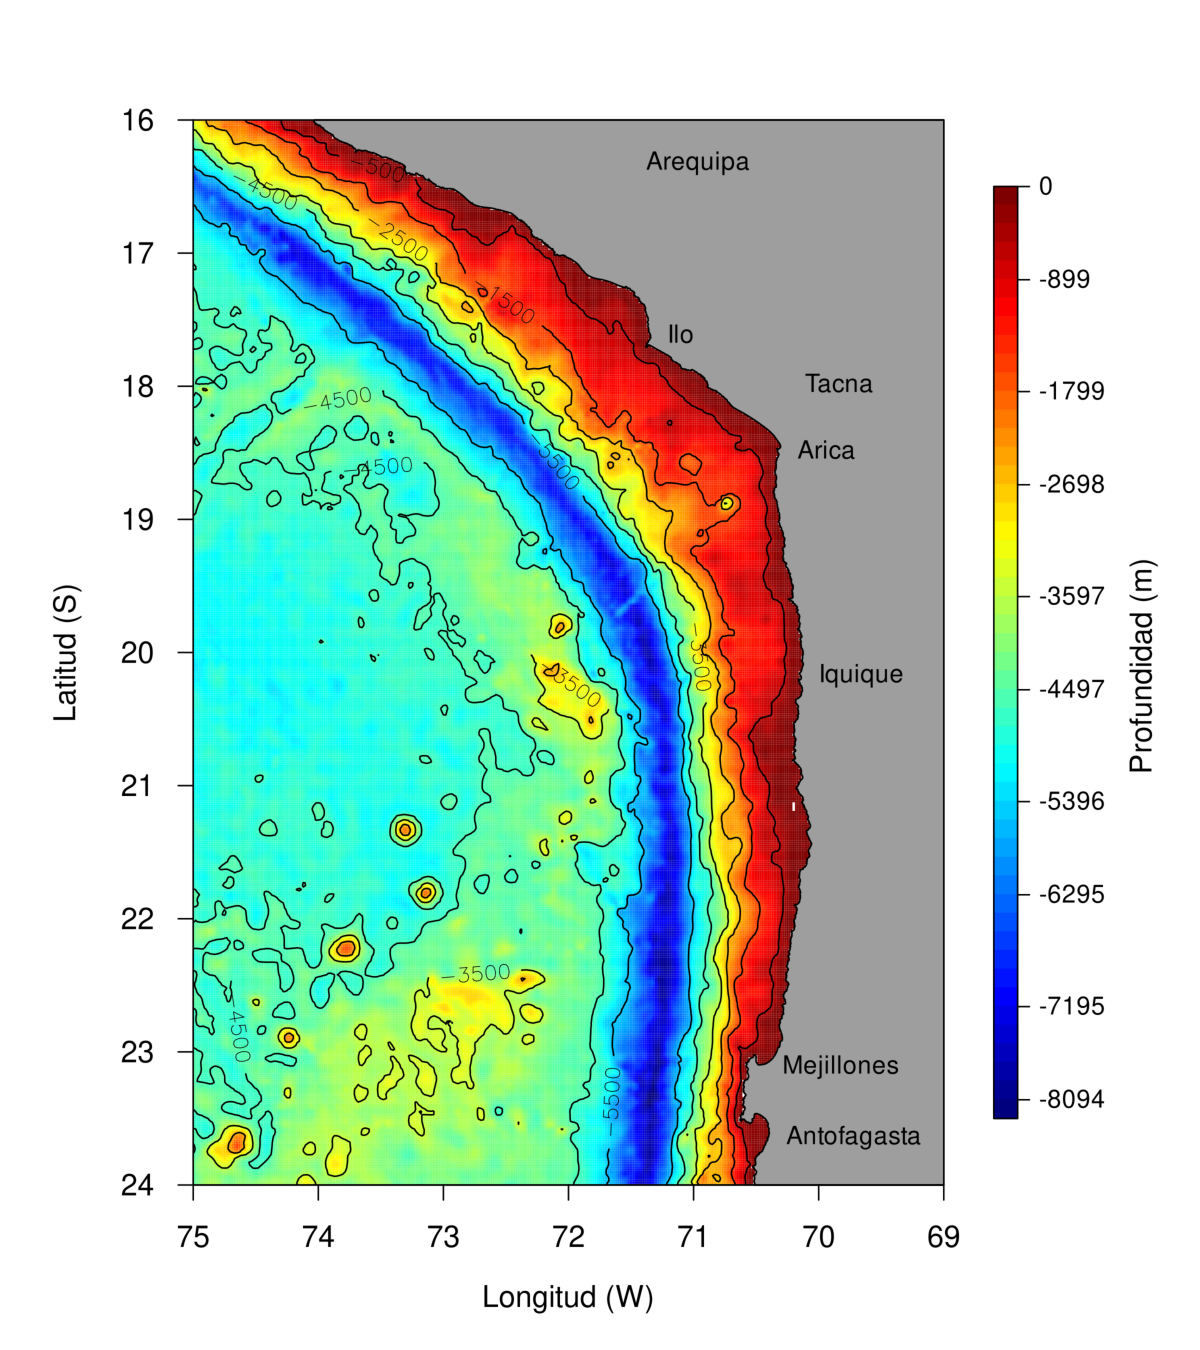
\includegraphics[width=14cm,height=10cm]{Figuras/figura1.pdf}
 \caption{\'Area de distribuci\'on del stock de anchoveta del sur de Per\'u y norte de Chile, distribuido entre los 16\degree LS - 24\degree LS (FUENTE: Modelo Global de Elevaci\'on Batim\'etrico, ETOPO1-NOAA.}
 \label{Fig1}
\end{figure}

Es importante se\~{n}alar que el stock de anchoveta del sur de Per\'u y norte
Chile, se plantea como un stock independiente del stock de anchoveta de
la III y IV regi\'on (Leal y Canales, 2014). Canales y Leal (2009)
plantean que la anchoveta centro-norte podr\'ia corresponder a una unidad
poblacional independiente de la ubicada al norte de los 25\degree LS, que
recluta, crece y se reproduce en el \'area. Aunque no se reportan estudios
formales a contestar esta pregunta, existen antecedentes que permiten
plantear la hip\'otesis de su independencia del stock sur de Per\'u y norte
de Chile. Los cruceros oceanogr\'aficos desarrollados en la d\'ecada de 1980
muestran focos discretos de desove (huevos y larvas) de anchoveta en las
bah\'ias de Caldera y Coquimbo (Rojas \textit{et al}., 1983). Esto sugiere
que la zona centro-norte de Chile podr\'ia representar un h\'abitat
favorable para la anchoveta particularmente en las bah\'ias de Caldera y
Coquimbo, donde existen patrones de circulaci\'on y focos de surgencia
(Valle-Levinson y Moraga, 2006) que podr\'ian facilitar la retenci\'on y
desarrollo de la anchoveta en estas bah\'ias. Serra y Gil (1975)
estudiaron la migraci\'on del stock de la anchoveta del sur de Per\'u y
norte de Chile mostrando la ocurrencia de intensos y amplios movimientos
migratorios hacia el sur de Per\'u en invierno y verano. Menos intensos y
amplios son los movimientos migratorios de anchoveta con direcci\'on hacia
los 24\degree LS. Un estudio similar fue realizado en 1997 (Mart\'inez
\textit{et al}., 1998) mostrando similares resultados en t\'erminos de
direcci\'on e intensidad de las migraciones. Se plantea que en la zona
comprendida entre los 24\degree LS y 25\degree LS al parecer no
existir\'ian las condiciones oceanogr\'aficas para permitir un flujo
continuo que permita la residencia de focos anchoveta entre ambas zonas
(Serra, com. pers.). Las poblaciones de Caldera y Coquimbo habr\'ian
surgido cuando en algunos a\~{n}os (y por razones ambientales, e.i. El
Ni\~{n}o), la anchoveta de la zona norte expande su distribuci\'on hacia el
sur de los 24\degree LS, colonizando las bah\'ias de Caldera y Coquimbo
donde procesos oceanogr\'aficos permiten el crecimiento y desarrollo de
poblacionales locales de anchoveta. Sin embargo, esta hip\'otesis no ha
sido demostrada a\'un. \vspace{0.5cm}

En esta zona, la surgencia costera del norte de Chile se caracterizada
por ser d\'ebil y continua (Blanco \textit{et al}., 2001), con altos
valores de clorofila (5 mg m$^{-3}$) restringidos a una estrecha banda
costera (20 km desde la costa), con un m\'aximo ciclo anual
en primavera-verano que es coincidente con el m\'aximo ciclo anual del
viento (Hormazabal \textit{et al}., 2001; Correa-Ram\'irez
\textit{et al}., 2007; Correa-Ram\'irez \textit{et al}., 2012). El ciclo
de vida de la anchoveta est\'a asociado a temperaturas que van desde los
12\degree a 23\degree C (Silva \textit{et al}., 2012; Claramunt
\textit{et al}., 2012), con una distribuci\'on dentro de las 50 mn de la
costa y donde casi el 70\% de las capturas de la flota industrial se
desarrolla dentro de las primeras 20 mn durante los \'ultimos diez a\~{n}os
(B\"ohm \textit{et al}., 2016). En esta franja costera la productividad
biol\'ogica es alta debido al incremento de la abundancia del plancton
producto de la surgencia costera. En la escala interanual, el principal
forzante f\'isico est\'a asociado con ciclo ENOS que determina una baja
captura producto de una profundizaci\'on de la anchoveta afectando su
disponibilidad y accesibilidad. Adem\'as, durante un evento c\'alido la
anchoveta presenta un desplazamiento al sur de la zona de estudio (Y\'a\~{n}ez
\textit{et al}., 1995; \~{N}iquen y Bouchon, 2004).


\subsection{Unidades de stock}

Recientes estudios han determinados el n\'umero de unidades poblacionales
(demogr\'aficas) de anchoveta \textit{Engraulis ringens} desde la regi\'on
de Arica hasta la de Los Lagos, a trav\'es de la aplicaci\'on de m\'ultiples
metodolog\'ias de an\'alisis: an\'alisis qu\'imico de otolitos (is\'otopos
estables y microelementos), fauna parasitaria, an\'alisis de micro
incrementos de otolitos, morfolog\'ia de otolitos y an\'alisis de marcadores
moleculares. La integraci\'on de los m\'etodos de an\'alisis mostr\'o fuerte
evidencia de que la zona 3 (Valpara\'iso-Los Lagos) corresponde a una
unidad demogr\'afica claramente separada de las zonas 1
(Arica-Antofagasta) y 2 (Copiap\'o-Coquimbo), con niveles de mezcla
inferiores al 5\%, mientras que se encontr\'o evidencia de que las zonas 1
y 2 presentan niveles mayores de mezcla, entre 21 y 26\%. Adem\'as, se
debe considerar que las tasas de mezcla antes se\~{n}aladas pueden variar a
escala interanual y que pueden ser producto de dispersi\'on durante las
fases tempranas de huevos y larvas; y/u otros procesos advectivos que
afecten las primeras fases de la progenie siendo adem\'as afectadas por
cambios ambientales y/o en el tama\~{n}o de la poblaci\'on (Niklitschek
\textit{et al}. 2017).


\subsection{Reproducci\'on}

La anchoveta es un desovante parcial, es decir, en un periodo
determinado es posible encontrar ejemplares en diferentes estados de
madurez sexual. Adem\'as, la anchoveta desova en tandas para producir un
vasto n\'umero de peque\~{n}os huevos sobre un extenso periodo de desove que
va desde mediados de agosto hasta el verano (Plaza \textit{et al}.,
2012; Claramunt \textit{et al}., 2012), con una m\'axima intensidad que
ocurre desde agosto a septiembre y otra desde diciembre a enero
(Contreras-Reyes \textit{et al}., 2016). En este extenso periodo de
desove (\textbf{Figura \ref{Fig2}}), en el cual el 60\% del ciclo anual
el \'indice gonadosom\'atico est\'a por un valor sobre 5 (valor que se\~{n}ala que
el 90\% o m\'as de las hembras est\'an sexualmente activas, confirmado
mediante an\'alisis histol\'ogico), la anchoveta desova en sitios asociados
a altas concentraciones de clorofila (Claramunt \textit{et al}., 2012),
ya que esta variable ambiental es un buen indicador de la producci\'on
primaria (Longhurst \textit{et al}., 1995) y por ende de la
disponibilidad de alimento. Basilone \textit{et al}. (2006) demostraron
que los niveles de clorofila afectan la intensidad del desove y el
factor de condici\'on. La madurez a la talla de la anchoveta ha sido
estudiada por Martinez \textit{et al}. (2009), cuya talla media de
madurez corresponde a 11.5 cm en longitud total.

\vspace{0.5cm}
\begin{figure}[htb!]
 \centering
 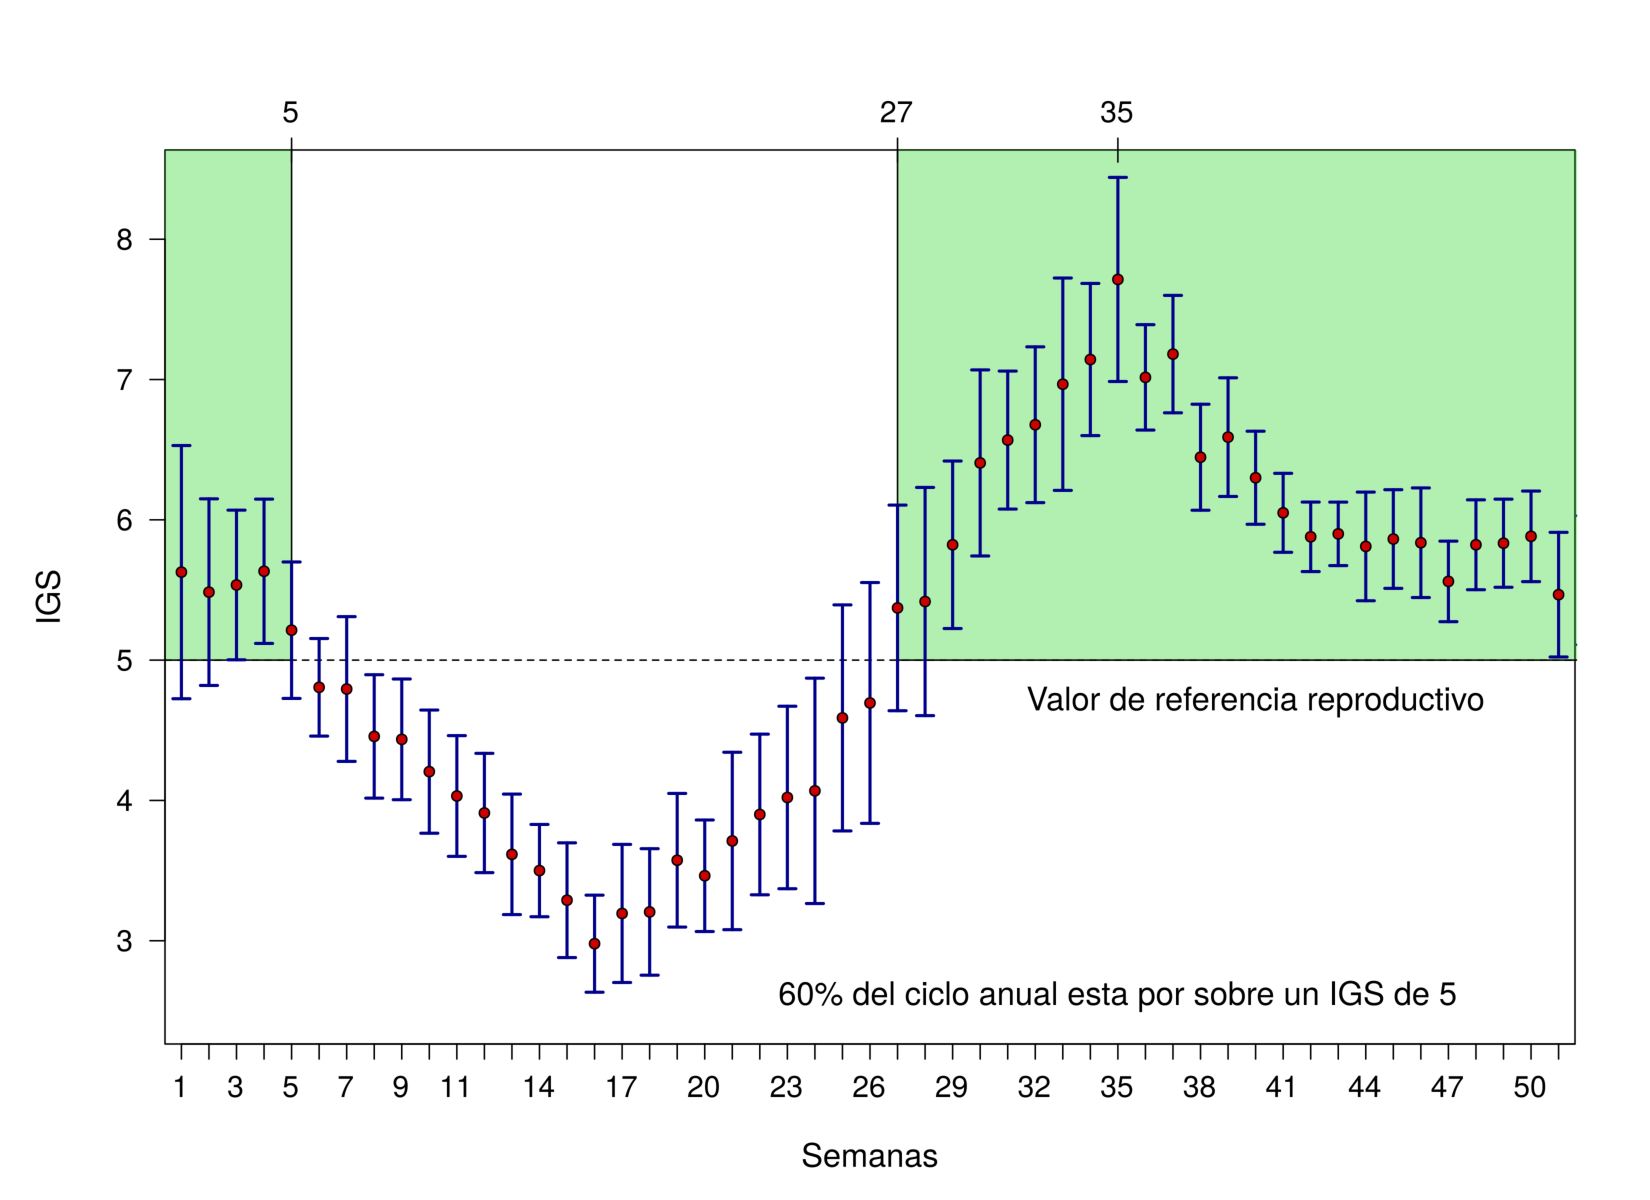
\includegraphics[width=12cm,height=8cm]{Figuras/figura2.pdf}
 \caption{Ciclo anual del \'indice gonadosom\'atico en escala semanal construido a partir de los datos recolectados por el monitoreo reproductivo en la zona norte de Chile desde el a\~{n}o 2000 al 2018. La l\'inea punteada en un valor de 5 se\~{n}ala el inicio de la actividad biol\'ogica (FUENTE: IFOP).}
 \label{Fig2}
\end{figure}


\subsection{Reclutamiento}

Se define como reclutas a los ejemplares menores a 11.5 cm de longitud
total e hist\'oricamente el ingreso de estos se ha observado desde octubre
hasta marzo, sin embargo, durante los \'ultimos a\~{n}os se ha detectado una
mayor presencia de reclutas desde abril hasta agosto (B\"ohm
\textit{et al}., 2016). Sin embargo, la distribuci\'on de longitudes
observada por el crucero hidroac\'ustico estim\\o un 73\% de reclutas,
distribuy\'endose los ejemplares entre 2.5 y 16 cm (Leiva \textit{et al}.,
2016), con una alta presencia de individuos de 2.5 y 5 cm asociados a la
franja costera. Durante la fase c\'alida del evento ENOS se observa un
alto porcentaje de ejemplares menores a los 12 cm, alcanzando un 70\% la
presencia de reclutas en las capturas de la flota industrial (Bertrand
\textit{et al}., 2004; B\"ohm \textit{et al}., 2016). Adem\'as, durante el
\'ultimo tiempo se ha observado una disminuci\'on de las tallas medias en la
flota industrial, donde la falta de ejemplares adultos ha estado ausente
en los \'ultimos a\~{n}os. La distribuci\'on de longitudes en las capturas de la
flota industrial chilena muestra un patr\'on unimodal con una talla media
de 14.7, 14.1, 13.0, 12.1, 12.6, 13.2, 11.4 y 11.5 cm en el 2013, 2014,
2015, 2016, 2017, 2018, 2019 y 2020 respectivamente. Durante los \'ultimos
diez a\~{n}os, la biomasa de este recurso ha registrado una importante
reducci\'on producto de una tendencia negativa en los reclutamientos y un
aumento de la mortalidad por pesca (Esp\'indola y Quiroz, 2017). Sin
embargo, en los \'ultimos cruceros de evaluaci\'on directa realizados en la
zona norte de Chile han registrado biomasas de reclutas por sobre el
promedio hist\'orico, cambiando la tendencia de anomal\'ias negativas a
positivas en los reclutamientos. Esto debido principalmente a que el
reclutamiento del 2016 es uno de los mayores registrados en la \'ultima
d\'ecada, superior en un 24\% al reclutamiento observado en el 2015, y muy
similar al observado en el 2014. Es decir, durante los a\~{n}os 2015-16-17
se han registrado un valor medio de 241 ($\pm$) 28 mil toneladas de
reclutas. Aunque, la biomasa de reclutas observados a finales del
segundo semestre del 2017 alcanz\'o un valor cercano a las 41 mil
toneladas (Leiva \textit{et al}., 2018), lo que representa una
disminuci\'on del 84\% con respecto a la estimaci\'on de biomasa de reclutas
hecha en el primer semestre del 2017. Sin embargo, a finales del 2018 se
registr\'o un valor de 596 mil toneladas de reclutas, valor m\'as alto de la
serie historia desde que se hace el crucero ac\'ustico (1996) en el norte
de Chile.


\subsection{Alimentaci\'on}

La anchoveta se alimenta de fitoplancton y zooplancton, con una alta
predominancia de fitoplancton por sobre zooplancton en 2.5 \'ordenes de
magnitud (Medina \textit{et al}., 2015). Los componentes de mayor
importancia relativa en la dieta fueron las diatomeas en el fitoplancton
y los cop\'epoda dentro del zooplancton, con un claro patr\'on oportunista y
depredador generalista de la anchoveta en la zona norte de Chile.
Durante los estadios larvales, el principal \'item alimenticio es el
fitoplancton y posteriormente el zooplancton (Y\'a\~{n}ez-Rubio
\textit{et al}., 2011).


\subsection{Crecimiento}

Estudios recientes, utilizando an\'alisis de microestructura de los
otolitos, han reportado un crecimiento muy acelerado en la fase juvenil
en algunas especies, incluido \textit{Engraulidos}, lo que parece ser
indicativo que estas especies alcanzan una porci\'on significativa de sus
longitudes asint\'oticas al finalizar el primer a\~{n}oo de vida (Cerna y
Plaza, 2016). En este contexto, se ejecut\'o el proyecto FIP 2009-17 que
buscaba ajustar la asignaci\'on de edad anual, desde el an\'alisis de
microestructura de otolitos, que permitiera consignar la edad correcta
de ejemplares que son producto de un reclutamiento prolongado en la zona
norte de Chile. Los juveniles de esta especie crecieron a tasas muy
elevadas, donde los reclutas de entre 11 y 12 cm de longitud total
ten\'ian entre 4 y 5 meses de edad. Tambi\'en se pudo determinar la edad
diaria en ejemplares mayores a 12 cm de longitud total, report\'andose que
ejemplares de entre 15 y 16 cm no ten\'ian m\'as de 400 d\'ias de vida.
Posteriormente, un segundo proyecto de investigaci\'on fue ejecutado
(SUBPESCA No 4728-31 LP 11), el cual permiti\'o validar la periodicidad
diaria de formaci\'on de los micro incrementos primarios en juveniles y
adultos de esta especie en condiciones de confinamiento, lo que
ratificaba los resultados del FIP 2009-17. Y Finalmente, un \'ultimo
proyecto FIP 2014-31 permiti\'o confirmar la determinaci\'on y asignaci\'on de
la edad de la anchoveta en la XV-II Regiones. Este proyecto concluy\'o que
la determinaci\'on de la edad a nivel diario es altamente confiable para
la anchoveta, \textit{Engraulis ringens}, en la zona norte de Chile.
Esta secuencia de proyectos involucrados en la determinaci\'on de la edad
de la anchoveta es mostrada en la \textbf{Figura \ref{Fig3}}.

\vspace{0.5cm}
\begin{figure}[htb!]
 \centering
 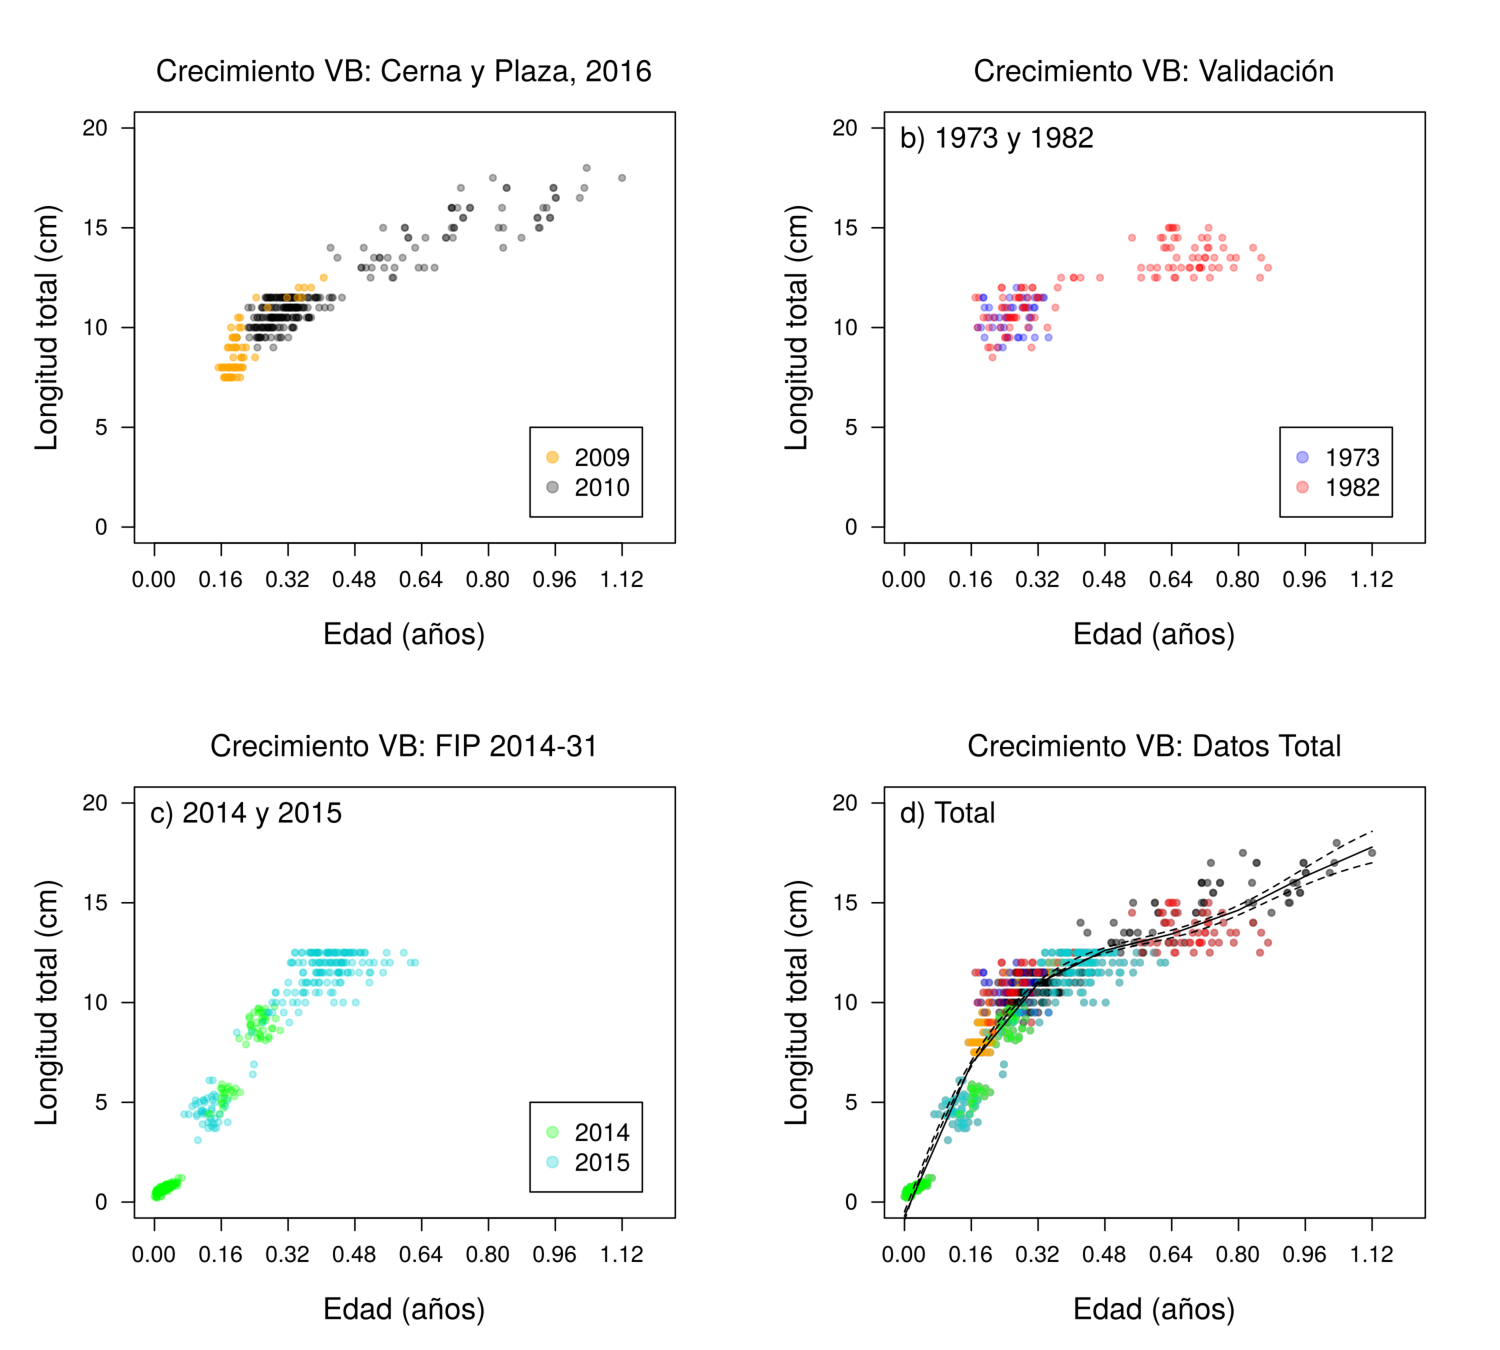
\includegraphics[width=16cm,height=12cm]{Figuras/figura3.pdf}
 \caption{Diferentes proyectos que dan cuenta del modelo de crecimiento de la anchoveta en la zona norte de Chile, en el panel d) se resumen todos los datos juntos de los diferentes proyectos.}
 \label{Fig3}
\end{figure}

Tambi\'en se han usado otolitos de peces de anchoveta capturados entre
enero y julio del 2015, cuyos 47 otolitos se les cont\'o el n\'umero de
incrementos desde el segundo anillo conc\'entrico que rodea el primordio
central hasta el borde del otolito. Las fechas de nacimiento fueron
calculadas substrayendo a la fecha de captura la edad total en d\'ias. Los
peces capturados correspondieron a juveniles de entre 8.5 y 12.5 cm de
longitud total con edades que fluctuaron entre 97 y 167 d\'ias, que
corresponden a peces nacidos entre julio y diciembre del 2014 y una
menor cantidad entre enero y abril (B\"ohm \textit{et al}., 2016).
Entonces, la edad de reclutamiento de la anchoveta var\'ia entre los 92
(3er mes) y 191 d\'ias (6to mes) desde la eclosi\'on. Estos resultados son
coincidentes con los reportados por Simpson y Buzeta (1967) que se\~{n}alan
dos nacimientos, uno durante el oto\~{n}o (feb-abr) y el otro en primavera
(jul-nov), con un coeficiente de crecimiento (k) de 1.6 a\~{n}o$^{-1}$ y
una longitud asint\'otica (L$_{inf}$) de 16.9 cm. Tambi\'en Saetersdal y
Valdivia (1964) reportan para el Per\'u una descendencia de verano y otra
de primavera, con la entrada de peces juveniles durante octubre-enero y
otra en marzo-junio, esta \'ultima contiene una alta proporci\'on de peces
de peque\~{n}o tama\~{n}o por debajo de los 12 cm.

Reconfigurando los datos de micro incrementos diarios (otolitos) hacia
una escala de paso de tiempo mensual, como se puede apreciar en la
\textbf{Figura \ref{Fig4}}, esta indica que a los tres meses de edad hay
individuos de 4 y 12 cm de longitud total dependiendo del a\~{n}o en que
fueron recolectados los peces, mostrando la alta variabilidad que
presenta el crecimiento de la anchoveta en los primeros meses de vida.
Estos resultados indican que habr\'ia individuos madurando sexualmente a
los 3 meses para los a\~{n}os 1973, 1982 y 2009. En cambio, para los seis
meses de edad, m\'as de la mitad de los individuos (64\%) est\'an maduros
sexualmente (caja celeste en la \textbf{Figura \ref{Fig4}}).

\vspace{0.5cm}
\begin{figure}[htb!]
 \centering
 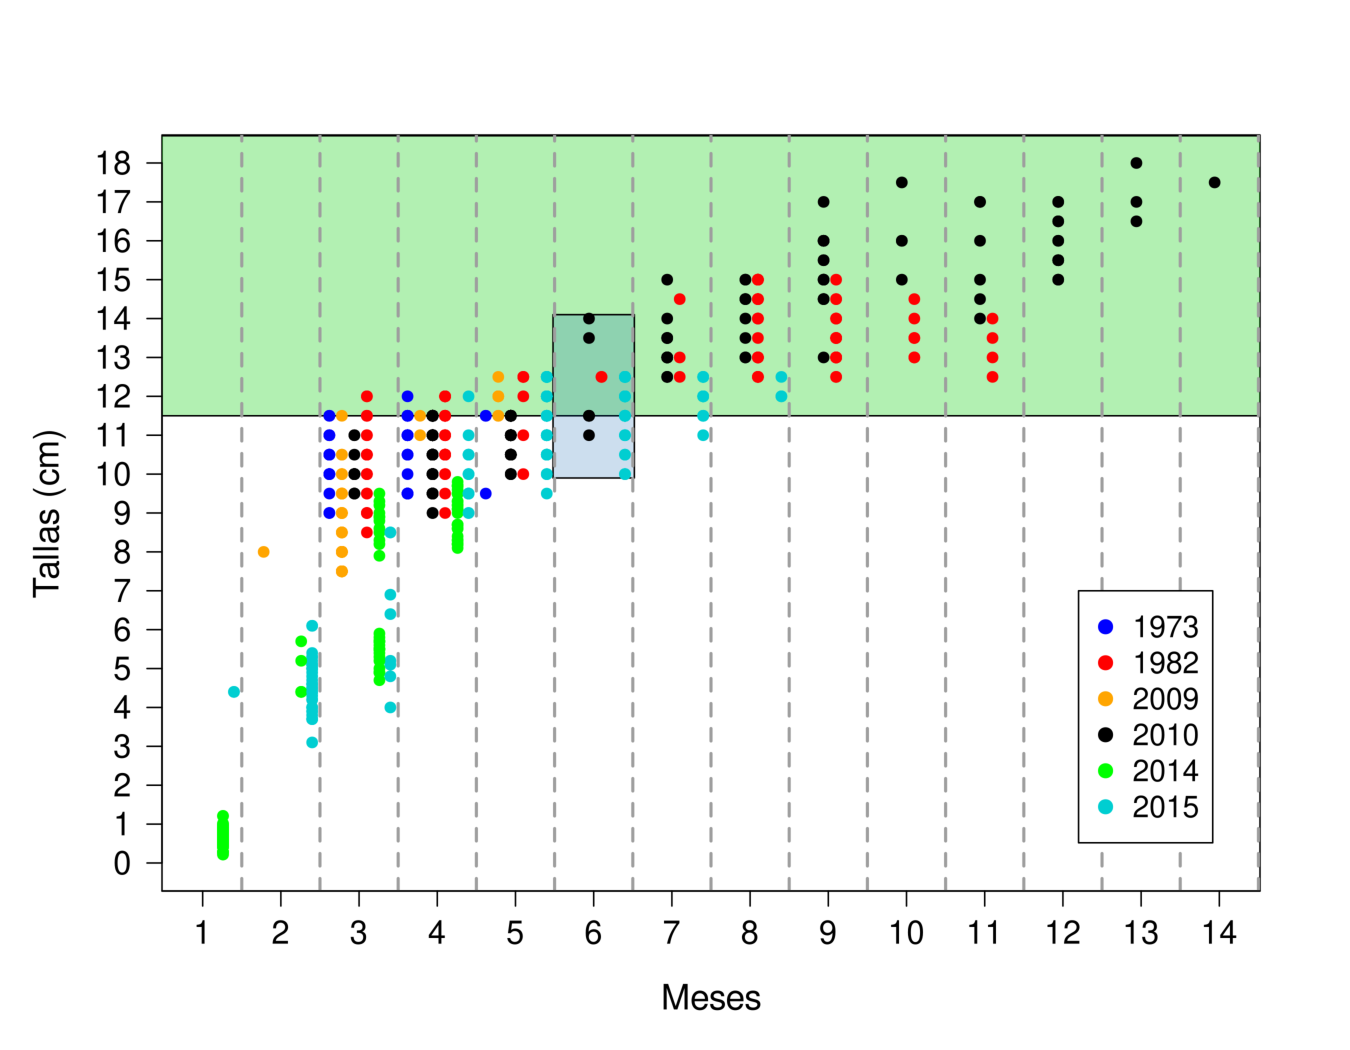
\includegraphics[width=11cm,height=7cm]{Figuras/figura4.pdf}
 \caption{Reconfiguraci\'on de los datos de crecimiento de la anchoveta de la zona norte de Chile a una escala de tiempo mensual. La caja verde contiene los individuos sexualmente maduros que corresponde a tallas mayores e igual a 11.5 cm. Y la caja celeste contiene a los individuos de seis meses de edad con un intervalo de tallas que va desde los 10 a 14 cm de longitud total.}
 \label{Fig4}
\end{figure}


\subsection{Variabilidad ambiental}

Una de las principales caracter\'isticas que presentan los peque\~{n}os peces
pel\'agicos es su alta variabilidad en el tama\~{n}o de su poblaci\'on debido a
las fluctuaciones ambientales en diferentes escalas de espacio y tiempo.
El principal forzante de los cambios interanuales de las condiciones
atmosf\'ericas y oceanogr\'aficas est\'a asociado al fen\'omeno El Ni\~{n}o
Oscilaci\'on del Sur (ENOS). Durante la fase c\'alida del ENOS se produce
una disminuci\'on de la abundancia relativa de la anchoveta, con una
profundizaci\'on y distribuci\'on m\'as costera, afectando la disponibilidad a
la flota industrial. Adem\'as, de una alta presencia de juveniles por
sobre los adultos (Bertrand \textit{et al}. 2004). Durante la \'ultima
fase c\'alida del ENOS (2015- 16) se observ\'o una talla modal de 12.5 cm en
las estructuras de las capturas de la flota industrial (CIAM, 2017)
donde los ejemplares mayores a 16 cm no fueron observados. Es decir, las
tallas medias han ido disminuyendo durante los \'ultimos a\~{n}os y los buenos
reclutamientos observados en los tres \'ultimos cruceros no se han
traducido en ejemplares adultos, lo que refleja un claro efecto del
calentamiento de la temperatura del mar debido a la fase c\'alida del
ENOS. Y m\'as a\'un, si consideramos los efectos del cambio clim\'atico
(Bowler \textit{et al}., 2017) y la alta probabilidad de que eventos
El Ni\~{n}o se hagan m\'as frecuentes como resultado del calentamiento
global (Hansen \textit{et al}., 2006; Cai \textit{et al}., 2014).


\subsection{Ciclo de vida de la anchoveta}

Considerando la informaci\'on previamente se\~{n}alada en el punto 2, en el
sentido de: i) una distribuci\'on principalmente costera, donde el 70\% de
las capturas se desarrolla dentro de las primeras 20 millas n\'auticas en
los \'ultimos diez a\~{n}os, ii) con un desove que ocurre en un extenso
periodo que va desde primavera hasta el verano, con dos m\'aximos de
intensidad, uno que ocurre desde agosto a septiembre y el otro desde
diciembre a enero, es decir, dos reclutamientos al a\~{n}o iii) una
alimentaci\'on basada principalmente en el fitoplancton y secundariamente
en el zooplancton, donde los componentes de mayor importancia relativa
en la dieta son las diatomeas en el fitoplancton y los cop\'epoda en el
zooplancton, con un claro patr\'on oportunista y depredador generalista,
iv) los nuevos antecedentes que dan cuenta de un coeficiente de
crecimiento de la ecuaci\'on de von Bertalanffy de k = 1-2 a\~{n}o$^{-1}$,
donde al a\~{n}o de vida alcanza una longitud media de 16.3 cm y v) una
mortalidad natural de 2.2 a\~{n}o$^{-1}$. Entonces, en base a estos
antecedentes expuestos se plantea el siguiente modelo conceptual de la
historia de vida de la anchoveta (\textit{Engraulis ringens}) para el
sur de Per\'u y norte de Chile (\textbf{Figura \ref{Fig5}}).

\vspace{0.5cm}
\begin{figure}[htb!]
 \centering
 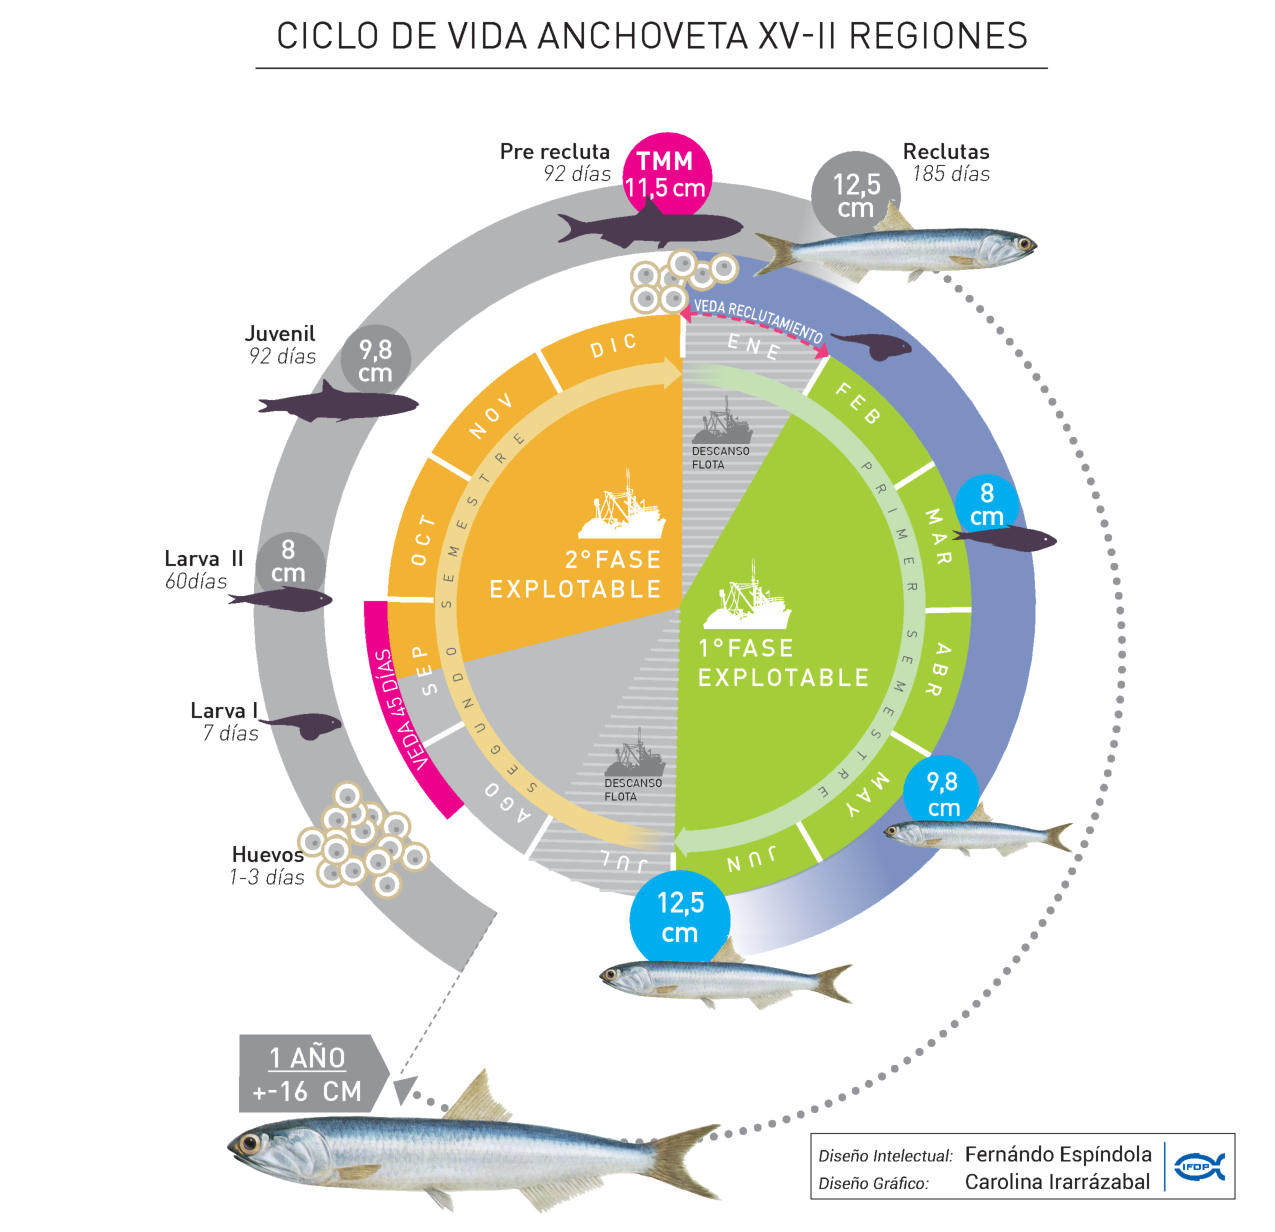
\includegraphics[width=17cm,height=13cm]{Figuras/figura5.pdf}
 \caption{Diagrama del modelo conceptual planteado para la anchoveta (\textit{Engraulis ringens}) del sur de Per\'u y norte de Chile (XV-II Regiones)}
 \label{Fig5}
\end{figure}


\subsection{Pesquer\'ia}

La anchoveta es el recurso objetivo de la pesquer\'ia pel\'agica de cerco de
la zona norte de Chile, localizada en la Regi\'on de Arica y Parinacota,
Regi\'on de Tarapac\'a y la Regi\'on de Antofagasta. La pesquer\'ia de anchoveta
del norte de Chile (18\degree 20'LS - 24\degree 00'LS) ha reportado en
promedio 1.271 ($\pm$ 713 mil) millones de toneladas anuales de
desembarque desde el a\~{n}o 1984 hasta el 2017, lo que representa una alta
importancia a la econom\'ia regional y de empleos directos e indirectos,
con el consiguiente beneficio econ\'omico y social. Los desembarques de la
anchoveta en el norte de Chile han presentado fuertes variaciones en la
historia de la pesquer\'ia, en particular, las capturas fueron bajas en el
2009 y 2010 alrededor de un 46\% bajo el promedio 1984-2012 de 809 mil
toneladas. Esta situaci\'on tambi\'en se observ\'o en la pesquer\'ia del sur del
Per\'u donde en particular los a\~{n}os 2010 y 2013 se observ\'o una disminuci\'on
de las capturas de m\'as de un 47\% bajo el promedio 1984-2012 de 552 mil
toneladas. A pesar de que el desembarque de ambos pa\'ises sufri\'o un
incremento relativo en el a\~{n}o 2011 (1.5 millones de toneladas), en el
a\~{n}o 2012 y 2013 se observ\'o una disminuci\'on del desembarque total
respecto al 2011. Durante el a\~{n}o 2014 (1 mill\'on de toneladas) se observ\'o
un repunte del desembarque respecto de semestres equivalentes en a\~{n}os
anteriores. En el 2015, el desembarque disminuye leventemente para
alcanzar las 926 mil toneladas, pero en el 2016 se registr\'o el valor m\'as
bajo durante los \'ultimos diecisiete a\~{n}os, con un registro cercano a las
397 mil toneladas totales (\textbf{Figura \ref{Fig6}}). Durante el 2017
este valor aumenta por sobre las 700 mil toneladas anuales para el stock
compartido de anchoveta, sin embargo, en el 2018 este valor aumenta
hasta las 971 mil toneladas anuales, superando la cuota de captura en
211 mil toneladas. En el 2019 este valor alcanzo las 719 mil toneladas,
valor por debajo de la cuota correspondiente a 760 mil toneladas. Y en
el 2020, este valor cae a las 271 mil toneladas.

Estacionalmente, el an\'alisis promedio hist\'orico (2008-2012) de las
capturas de anchoveta se\~{n}alan que \'estas se concentran en los siete
primeros meses del a\~{n}o, aportando con el 87\% del volumen del a\~{n}o,
situaci\'on distinta a lo observado en los \'ultimos a\~{n}os donde \'estos se han
focalizado en s\'olo dos a tres meses. Al respecto, en el 2014 el 89\% de
los desembarques se registraron en abril y mayo, mientras que en el 2015
el 78\% se concentr\'o en mayo y junio. En el 2016 el 73\% de las capturas
se focaliz\'o en mayo y junio, siendo nulos a partir de septiembre para la
regi\'on sur del Per\'u. En el norte de Chile, la captura de anchoveta se
concentra en los meses de marzo (2014) y abril (2015). En cambio, en el
a\~{n}o 2016 el 77\% de las capturas se concentraron en cuatro meses
(abril-julio), siendo junio el valor m\'aximo. En el 2017, el 60\% de las
capturas se concentraron en tres meses (feb-abr), con marzo con el mes
de m\'axima captura.

\vspace{0.5cm}
\begin{figure}[htb!]
 \centering
 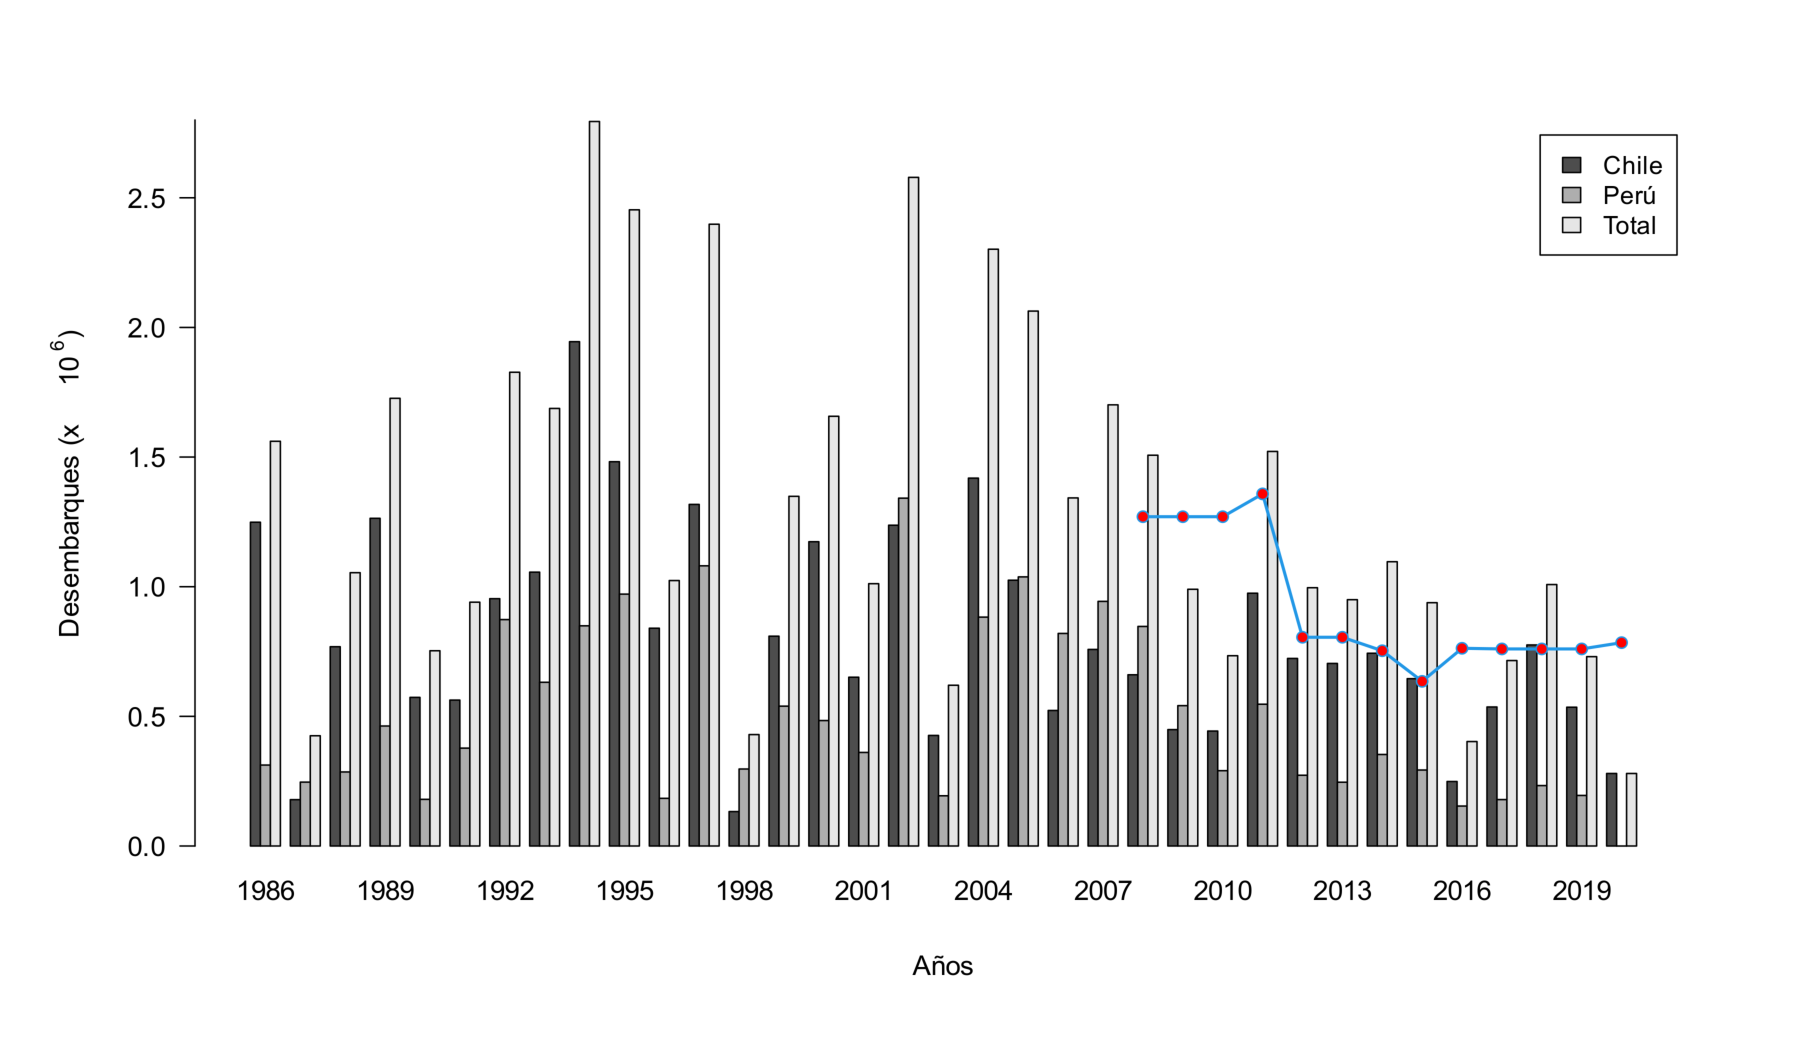
\includegraphics[width=13cm,height=8cm]{Figuras/figura6.pdf}
 \caption{Desembarques (t) por pa\'is para el stock de anchoveta del sur de Per\'u y norte de Chile. Los puntos rojos indican las cuotas de capturas asignadas para esta pesquer\'ia.}
 \label{Fig6}
\end{figure}


\subsection{Evaluaci\'on de stock}

Desde el a\~{n}o 2002 y hasta el 2010, la evaluaci\'on de stock de anchoveta
estuvo basada en un modelo estad\'istico de captura a la edad (MECE). En
octubre del 2010 se introdujo como una alternativa un modelo estad\'istico
de captura a la talla (MECT). Este cambio se debi\'o a las dudas
existentes en la asignaci\'on de la edad de la anchoveta, y tambi\'en porque
la escala anual no representaba de manera adecuada la din\'amica del
recurso debido al extenso periodo de desove, es decir, con un m\'aximo
marcado a mediados de agosto y otro de menor intensidad a comienzo del
a\~{n}o, \textbf{Figura \ref{Fig2}}, donde a comienzos del a\~{n}o el \'indice
gonadosom\'atico alcanzan valores mayores 6 y esta caracter\'istica del
desove hace que se observen reclutas durante todo el a\~{n}o.

Considerando estos aspectos y para independizarse de la determinaci\'on de
la edad se opt\'o por usar: i) la estructura de tallas de las capturas
como variables observadas, pero se continu\'o con una din\'amica en edades a
trav\'es de la simulaci\'on de una clave talla-edad, constante en el tiempo;
ii) para dar cuenta del extenso periodo de desove y de reclutas durante
gran parte de a\~{n}o, se trabaj\'o a escala semestral asumiendo la existencia
de dos reclutamientos y dos desoves por a\~{n}o. Estas dos modificaciones al
modelo de evaluaci\~{n}o de stock (MECE) llevaron a concluir que el modelo
MECT mejoraba el ajuste y adem\'as representaba mejor la din\'amica del
recurso (Serra y Canales, 2011). Una siguiente modificaci\'on al modelo de
evaluaci\'on tuvo lugar en septiembre de 2012 (Serra y Canales, 2012)
cuando se introdujo la diferenciaci\'on por flotas debido a que los
patrones de explotaci\'on parec\'ian ser distintos en Per\'u y Chile lo que se
observa en la composici\'on de tallas de la captura, esto a sugerencia del
Taller de Evaluaci\'on de Recursos de junio de 2012 (Serra y Canales,
2012). La modificaci\'on introducida si bien no gener\'o diferencias
significativas desde el punto de vista de las variables de estado del
stock y del ajuste del modelo, si permiti\'o representar mejor la
vulnerabilidad del stock por ambas flotas (Serra y Canales, 2013).

A pesar de las mejoras introducidas a la evaluaci\'on de stock de la
anchoveta y al hecho que el modelo es considerado en desarrollo, dada la
incertidumbre en la edad y en el crecimiento, y la falta de sensibilidad
del modelo a los \'indices de abundancia motivaron el Taller de Revisi\'on
de la Evaluaci\'on de Stock de Anchoveta del Norte de Chile con la
participaci\'on del experto internacional en evaluaci\'on de recursos
pesqueros Dr. Chris Francis (Canales \textit{et al}., 2014). El Taller
dio cuenta de la revisi\'on de los datos, el modelo de evaluaci\'on y la
identificaci\'on de las principales fuentes de incertidumbre. En la
oportunidad se revis\'o cada fuente de informaci\'on utilizada en la
evaluaci\'on, y se realizaron algunas modificaciones buscando consistencia
y evidencia entre el (los) indicador (es) y el proceso modelado. Se
examin\'o el modelo de evaluaci\'on y sus supuestos estableci\'endose un
modelo base el cual estuvo asentado en una modificaci\'on del MECT
considerando dos flotas (Serra y Canales, 2013) pero donde se ha
independizado la estimaci\'on de la tasa de crecimiento, $k$, de la longitud
asint\'otica (L$_{inf}$) siguiendo la aproximaci\'on de Schnute y Fournier
(1980). Posteriormente, y utilizando el modelo base se realiz\'o un
an\'alisis de sensibilidad a las piezas de informaci\'on y supuestos del
modelo. Esto permiti\'o identificar las principales fuentes de
incertidumbre en la evaluaci\'on y recomendaciones de estudios posteriores
orientados a mejorar la evaluaci\'on de stock de anchoveta.

Uno de los temas prioritarios durante muchos a\~{n}os ha sido la
incertidumbre asociada a la determinaci\'on de la edad de la anchoveta.
Estudios recientes han reportado que el recurso tiene un crecimiento m\'as
r\'apido que el usado en las evaluaciones de stock hist\'oricas. Este
crecimiento muestra que esta especie alcanza una porci\'on significativa
de su longitud asint\'otica al finalizar su primer a\~{n}o de vida (Plaza
\textit{et al}., 2017). Estos antecedentes inducen cambios relevantes en
la din\'amica de la especie, los que se ven reflejados en los casos de
evaluaci\'on de stock que fueron implementados en el primer informe de
estatus (Esp\'indola y Quiroz, 2017). En este informe se dio cuenta de
diez an\'alisis, seis en t\'erminos del crecimiento y cuatro en t\'erminos de
la productividad, determin\'andose que la mayor reducci\'on de la
verosimilitud total se produce en t\'erminos del crecimiento, con un
$k$ = 2.12 a\~{n}o$^{-1}$ y L$_{inf}$ = 17.55 cm.

Dado el nuevo modelo de crecimiento y la incertidumbre que este g\'enero
en la evaluaci\'on de stock, durante los d\'ias 11 al 13 de marzo del 2019
se realiz\'o el taller de revisi\'on por pares del stock de anchoveta del
sur de Per\'u y norte de Chile por el Dr. James Ianelli, experto del
centro de ciencia pesquera de Alaska de la NOAA (National Oceanic and
Atmospheric Administration). El taller dio cuenta de la revisi\'on de los
datos usados en la evaluaci\'on de stock, el crecimiento de la anchoveta
basado en micro incrementos diarios y el supuesto de mortalidad natural
usado, las hip\'otesis estructurales que definen el modelo conceptual de
la pesquer\'ia de la anchoveta del sur de Per\'u y norte de Chile. Adem\'as,
se revis\'o la din\'amica poblacional, los modelos de los procesos y error,
la configuraci\'on del modelo de evaluaci\'on. Y finalmente, se revisaron
los ajustes del modelo de evaluaci\'on a los datos usados, las variables
poblacionales estimadas por el modelo, el desempe\~{n}o del modelo, an\'alisis
retrospectivo, puntos biol\'ogicos de referencia y estatus del recurso
estudiado.

Posterior a la revisi\'on por pares hecha por el Dr. Ianelli, durante los
d\'ias 8 al 12 de julio del 2019 en dependencias del IFOP, Valpara\'iso, se
realiz\'o el taller de sensibilidad de la evaluaci\'on de stock frente a
diferentes casos de an\'alisis (benchmark) en la anchoveta del sur de
Per\'u y norte de Chile con la colaboraci\'on de la Dra. Carolina Minte-Vera
de la Comisi\'on Inter-Americana del At\'un Tropical (IATTC), cuyo objetivo
fue cooperar en la implementaci\'on de las sugerencias de mejoras
priorizadas en el proceso de revisi\'on por pares, en caso de que dicho
proceso no sugiera un cambio estructural del enfoque de modelaci\'on (s\'olo
mejoras al modelo actual). En su defecto, (si se sugiere un cambio
estructural del modelo) contribuir en el desarrollo e implementaci\'on del
modelo base. Como el Dr. Ianelli recomend\'o hacer mejoras al modelo
actual de evaluaci\'on y valido el enfoque de modelaci\'on empleado en las
\'ultimas evaluaciones. En este taller se implementaron las
recomendaciones emanadas de la revisi\'on pares y se exploraron otras
modificaciones para mejorar el modelo, y el resultado de este taller
propuso un modelo base que podr\'ia ser usado para el manejo pesquero.
Posterior a este taller, se ha continuado mejorando el modelo de
evaluaci\'on, debido al objetivo de este proyecto, el programa de
mejoramiento continuo de la calidad en la asesor\'ia cient\'ifica,
implementando una selectividad de tipo doble-normal, con la capacidad de
convertirse en log\'istica en caso que los datos as\'i lo ameritan, esta
mejora permite lidiar con las altas mortalidades por pesca que se
observan con el modelo log\'istico (las que alcanzan el l\'imite superior
establecido en el modelo) y que repercuten en el an\'alisis retrospectivo
cuando se registran las altas abundancias totales estimadas a trav\'es del
m\'etodo ac\'ustico y las bajas capturas que se registraron durante el
periodo 2015-2017. Adem\'as, se han introducidos mejoras en cuanto a los
datos usados por el modelo de evaluaci\'on, como es la incorporaci\'on de
los pesos medios variables por semestre desde el a\~{n}o 2001 en adelante.


\subsection{Estatus}

El estado de explotaci\'on del stock de anchoveta del sur de Per\'u y norte
de Chile fue evaluado conforme al est\'andar adoptado por el Comit\'e
Cient\'ifico T\'ecnicos (CCT) y es sustentado en la estimaci\'on de los Puntos
Biol\'ogicos de Referencia (PBR) especie-espec\'ificos. Los proxies al
Rendimiento M\'aximo Sostenido (RMS) son: i) la biomasa al rendiento
m\'aximo sostenido (B$_{RMS}$) es igual al 50\% de la biomasa desovante
virginal (BD$_{0}$) y ii) la mortalidad por pesca al RMS (F$_{RMS}$)
es aquella mortalidad por pesca que en el largo plazo produce el 55\% de
la biomasa desovante por recluta igual a F55\%BDPR (Beverton y Holt,
1957). Considerando estos PBR, la mortalidad por pesca muestra un patr\'on
fluctuante desde mediados de 1992, en varios periodos donde se registran
valores por sobre el F$_{RMS}$ y otros periodos por debajo del
F$_{RMS}$. Sin embargo, desde el 2010 a la fecha los valores se ubican
por debajo del F$_{RMS}$, generando con esto una condici\'on sin
sobrepesca (\textbf{Figura \ref{Fig7}}), y al \'ultimo semestre de la
evaluaci\'on la mortalidad por pesca se encuentra un 76\% por debajo del
objetivo de manejo. De igual manera, los resultados indican que la
reducci\'on de la biomasa ocurrida a mediados del 2008 y en 2016 llevaron
a la poblaci\'on a valores por debajo de la biomasa al RMS, generando con
ello un estado de sobreexplotaci\'on. Sin embargo, la reducci\'on de la
mortalidad por pesca observada durante los \'ultimos a\~{n}os y la alta
variabilidad observados en los reclutamientos han llevado a la poblaci\'on
a niveles por encima del punto biol\'ogico de referencia objetivo, y esto
se traduce que desde mediados del 2016 a la fecha ha variado en torno a
un 1.49 ($\pm$ 0.46). Al \'ultimo semestre de la evaluaci\'on la biomasa
desovante se encuentra un 71\% superior al objetivo de manejo, y dado
los niveles de incertidumbre, existe una nula probabilidad de que la
BD$_{2020.5}$ $>$ BD$_{RMS}$ (\textbf{Figura \ref{Fig7}}),
generando con ello un estado de subexplotaci\'on en biomasa desovante.

\vspace{0.5cm}
\begin{figure}[htb!]
 \centering
 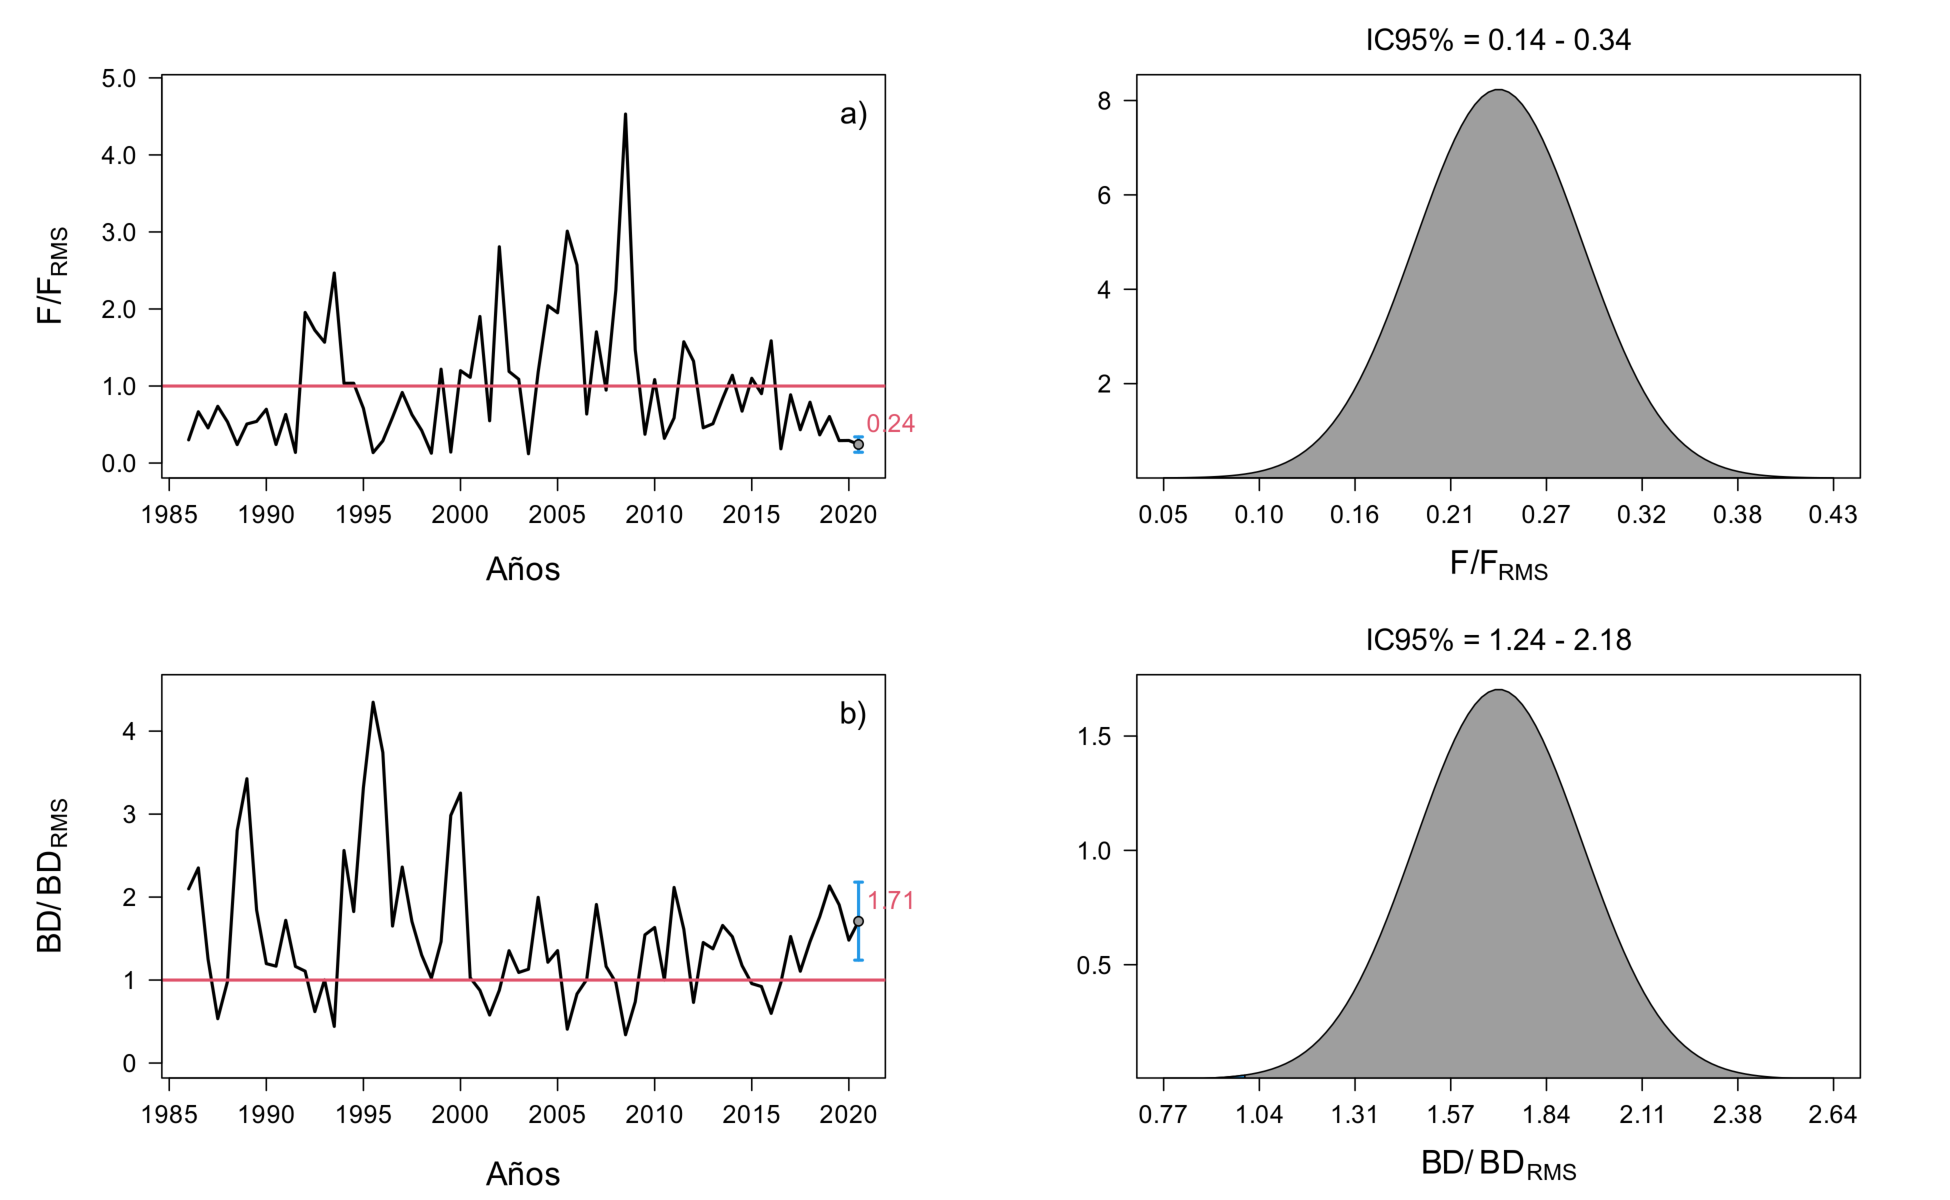
\includegraphics[width=14cm,height=10cm]{Figuras/figura7.pdf}
 \caption{Serie temporal de la raz\'on de la mortalidad por pesca respecto a su referente asociado al RMS y la incertidumbre al \'ultimo semestre de la evaluaci\'on en el planel superior (a) y la serie temporal de la raz\'on de la biomasa desovante respecto a su referente asociado al RMS y la incertidumbre al \'ultimo semestre de la evaluaci\'on en el panel inferior (b) para la anchoveta del sur de Per\'u y norte de Chile. La l\'inea roja representa el objetivo de manejo referido al RMS.}
 \label{Fig7}
\end{figure}


\subsection{Captura Biol\'ogicamente Aceptable (CBA)}

De acuerdo al ciclo de manejo hist\'orico de esta pesquer\'ia, la
recomendaci\'on de CBA comienza con el c\'alculo de la CBA inicial que
permite al CCT-PP, en octubre de cada a\~{n}o, establecer el estatus y
recomendar el rango de CBA para el a\~{n}o siguiente. En el mes de
diciembre, el crucero de evaluaci\'on hidroac\'ustico permite estimar la
abundancia y biomasa de reclutas de Chile (fines de a\~{n}o) y Per\'u
(primavera y verano), esta informaci\'on junto a datos provenientes de la
pesquer\'ia de Chile y Per\'u y la estimaci\'on de la biomasa desovante a
partir del m\'etodo de producci\'on diaria de huevos, es utilizada para la
actualizaci\'on de la CBA (marzo-abril).

La \textbf{Tabla \ref{Tab1}} muestra las CBA recomendadas por el CCT-PP
en las distintas etapas de establecimiento de cuotas, desembarques
registrados y sus diferencias, entre el 2015 y 2016. Entre el 2016 y
2019 se mantuvo una CBA statu quo en 760 mil toneladas, en ambos hitos
de manejo (CBA inicial y actualizada). El a\~{n}o 2020 se incrementa a 784
mil toneladas, no obstante, para ese a\~{n}o se captur\'o un 35\% de la CBA
recomendada.

\vspace{0.5cm}
\begin{table}[htb!]
 \caption{Captura biol\'ogicamente aceptables recomendadas por el CCT en las distintas etapas de establecimiento de CBA (ton), desembarques registrados (ton) y sus diferencias.}
 \label{Tab1}
 \centering
 \small
 \begin{tabular}{ccccc}
 \hline\noalign{\vskip 0.1cm}
 A\~{n}o & CBA inicial & CBA actualizada & Desembarques & Diferencia \\
 \hline\noalign{\vskip 0.1cm}
 2015 & 633.0 & 633.0$^{*}$ & 633.0 & 0.00 veces la CBA  \\
 2016 & 760.0 & 760.4$^{*}$ & 243.4 & 0.32 veces la CBA\\
 2017 & 760.0 & 760.0$^{*}$ & 529.7 & 0.70 veces la CBA  \\
 2018 & 760.0 & 760.0$^{*}$ & 751.1 & 0.99 veces la CBA  \\
 2019 & 749.3$^{*}$ & 749.3$^{*}$ & 524.9 & 0.70 veces la CBA  \\
 2020 & 784.3 & 784.3$^{*}$ & 271.9 & 0.35 veces la CBA  \\
 2021 & 564.4 & 743.7 & \---  & \---  \\
 \hline
 \textit{Nota:} & \multicolumn{1}{r}{$^{*}$status quo} \\
 \end{tabular}
\end{table}


\clearpage
\newpage

\section{METODOLOG\'IA DE TRABAJO}

\subsection{Objetivo espec\'ifico 1.}

\textit{\textquotedblright Implementar procedimientos de evaluaci\'on de stock basados en protocolos cient\'ificos para la determinaci\'on del estatus de anchoveta y sardina espa\~{n}ola, con arreglo al nivel de informaci\'on, conocimiento e incertidumbre correspondiente, conforme a los est\'andares actuales en ciencia pesquera.\textquotedblleft}
\vspace{0.5cm}

El enfoque de estudio se sustenta en la aplicaci\'on del m\'etodo cient\'ifico
y en el uso de la mejor informaci\'on y conocimiento disponible del
recurso y la pesquer\'ia a la fecha de ejecuci\'ion, consecuente con la
aplicaci\'on del enfoque precautorio en las pesquer\'ias establecido por la
FAO (1997) y el enfoque ecosist\'emico (FAO, 2003). Con este prop\'osito, se
aplicar\'an procedimientos de trabajo cient\'ifico (i.e., transparente,
auditables y reproducibles) e inclusivos (talleres y reuniones de
trabajo grupales), con el fin de asegurar el cumplimiento del Proceso de
Asesor\'ia Cient\'ifica y que la Administraci\'on cuente con ella, en el
Proceso Decisional de Manejo de las principales pesquer\'ias nacionales.
Para el logro de los objetivos del proyecto, se revisar\'a toda la
informaci\'on cient\'ifica y t\'ecnica disponible.

Se considera la participaci\'on del equipo de trabajo en las reuniones que
para estos efectos establezcan los Comit\'e Cient\'ifico T\'ecnicos, as\'i como
todas las actividades que demanden las Revisiones por Pares Externos e
Independientes (RPEI) de estos estudios (tanto de expertos nacionales
como internacionales) u otros proyectos que correspondan a temas
relevantes al manejo pesquero, cuando corresponda. Las recomendaciones
de los revisores constituir\'an un Est\'andar Metodol\'ogico en la Evaluaci\'on
de un determinado recurso, cuyos protocolos se mantendr\'an vigentes hasta
que se considere necesario perfeccionarlos, conforme la recomendaci\'on
del Comit\'e Cient\'ifico T\'ecnico respectivo.

Para determinar el estatus de los recursos selectos, se considerar\'a lo
establecido por los Comit\'e Cient\'ifico T\'ecnicos sobre los requerimientos
t\'ecnicos que define los est\'andares de an\'alisis y evaluaci\'on para las
pesquer\'ias analizadas, conforme a los niveles de conocimiento,
informaci\'on y calidad de los datos disponibles para esos fines. En
aquellos casos en que el nivel de desarrollo del conocimiento, la
informaci\'on o los datos sean limitados o con altos niveles de
incertidumbre, de forma que limiten o impidan la aplicaci\'on en propiedad
de procedimientos de evaluaci\'on y an\'alisis con est\'andares altos (i. e.,
para datos ricos), se desarrollar\'an e implementar\'an procedimientos y
m\'etodos alternativos adecuados a la disponibilidad de informaci\'on con el
fin de determinar el estatus de los recursos que se encuentren en esta
condici\'on, los que propender\'an a reducir los niveles de incertidumbre
que perturben la toma de decisi\'on (sensu Carmichael y Fenske, 2010).

No obstante, lo anterior y con el prop\'osito de alcanzar el Est\'andar
Completo, se identificar\'an las brechas y limitaciones que impiden lograr
ese objetivo y se propondr\'an detalladamente las acciones que se
consideren necesarias para alcanzarlo, en el corto o mediano plazo,
seg\'un corresponda.


\subsubsection{Modelo conceptual}

La din\'amica poblacional es conceptualizada a trav\'es del modelo biol\'ogico
de la historia de vida de la anchoveta (\textit{Engraulis ringens}), que
es sustentado por los siguientes componentes:

\begin{itemize}
\def\labelenumi{\alph{enumi}.}

\item
  \textit{Distribuci\'on geogr\'afica}. Se asume que la poblaci\'on de
  anchoveta de los 16\degree - 24\degree S constituye una \'unica unidad de stock.
  Adem\'as, se considera que el stock de anchoveta es homog\'eneo al
  interior de esta \'area, donde el conjunto de individuos est\'a sujeto a
  la misma probabilidad de crecimiento y mortalidad, y donde la
  migraci\'on fuera del \'area no es importante.
\item
  \textit{Escala temporal}. Se asume una escala temporal semestral. Los
  supuestos sobre la escala de la din\'amica se sustentan sobre el hecho
  que la anchoveta es una especie de vida corta (al a\~{n}o de vida alcanza
  una longitud media de 16.3 cm), que tiene un periodo de desove bien
  prolongado, comenzando a mediados de agosto y extendi\'endose a trav\'es
  de toda la primavera para comenzar a declinar hacia fines del verano.
  El periodo prolongado de desove y los reclutamientos han determinado
  que la escala temporal de la din\'amica poblacional usada sea al menos a
  nivel de semestre.
\item
  \textit{Reproducci\'on}. Dada la extensi\'on del periodo de desove, que va
  desde primavera hasta el verano, se asume que los individuos del stock
  tienen dos eventos reproductivos discretos durante el a\~{n}o. La m\'axima
  intensidad del desove ocurre desde agosto a septiembre y otra desde
  diciembre a enero. Consistente con ello, el reclutamiento a la
  pesquer\'ia tambi\'en se observa durante gran parte del a\~{n}o, registr\'andose
  un m\'aximo reclutamiento durante enero y otro que ocurre en julio.
\item
  \textit{Reclutamiento}. El reclutamiento ocurre a la forma de un pulso
  de abundancia a comienzos de cada semestre y estimado a trav\'es de
  desviaciones de R$_{0}$.
\item
  \textit{Modelo de crecimiento}. El crecimiento es determinado a trav\'es
  del an\'alisis de micro incrementos diarios de los otolitos. Estos
  resultados indican que a un a\~{n}o de vida la longitud media deber\'ia ser
  de 16.3 cm (Cerna y Plaza, 2016; Plaza \textit{et al}., 2017).
\item
  \textit{Mortalidad natural}. La tasa de mortalidad natural se asume
  constante en el tiempo y a trav\'es de las edades. Se considera un valor
  de 2.2 a\~{n}o$^{-1}$. Valor que es obtenido a trav\'es de aplicaci\'on de
  diferentes m\'etodos bio-anal\'ogico que est\'an disponibles en la
  literatura (\href{http://barefootecologist.com.au/shiny_m.html}).
\item
  \textit{La mortalidad por pesca}. Es el resultado de la interacci\'on
  entre la mortalidad por pesca semestral y el patr\'on de explotaci\'on
  edad y flota (Chile, Per\'u) espec\'ifico. Se asume que los desembarques
  en esta pesquer\'ia es un buen sustituto de las capturas.
\end{itemize}

El modelo de evaluaci\'on de stock de anchoveta se basa en un an\'alisis
estad\'istico de la din\'amica poblacional donde las observaciones en tallas
son transformadas a edades por medio de una clave talla- edad variable
en el tiempo, adem\'as incorpora informaci\'on biol\'ogica y pesquera. La
informaci\'on que ingresa al modelo consiste en los desembarques totales y
datos de composici\'on de longitudes que son proporcionados por el
programa de monitoreo de las pesquer\'ias de peces pel\'agicos (Chile-Per\'u),
mientras que las evaluaciones ac\'usticas de verano proporcionan
informaci\'on de la biomasa total, junto a la composici\'on de abundancia
por rango de longitud. Adem\'as, se incorpora informaci\'on de la biomasa
total estimada en la zona sur del Per\'u por las evaluaciones ac\'usticas.
En base a esta informaci\'on el modelo de evaluaci\'on estima las variables
de estado representadas por la biomasa desovante (BD) y los niveles de
mortalidad por pesca (F) para cada una de las flotas, que junto a los
puntos biol\'ogicos de referencia (PBR) permiten determinar el estatus y
calcular la \textquotedblleft Captura Biol\'ogicamente Aceptable (CBA)\textquotedblright.

En la implementaci\'on del procedimiento de evaluaci\'on de stock se
utilizan protocolos cient\'ificos basados en la determinaci\'on de un
sistema de niveles o \textquotedblleft tiers\textquotedblright que permiten clasificar la informaci\'on
disponible de las especies y su pesquer\'ia, los cuales se han convertido
en una herramienta de uso com\'un en la asesor\'ia orientada al manejo
pesquero en la actualidad. Para estimar el Rendimiento M\'aximo Sostenible
(RMS) se utiliza la estrategia de niveles y de acuerdo con la
clasificaci\'on del est\'andar de informaci\'on se definen los PBR o \textquotedblleft proxy\textquotedblright
que ser\'an usados para determinar el estatus del recurso. La definici\'on
de los procedimientos de c\'alculo de los PBR y del marco de referencia
especie espec\'ificos se basan en el estudio \textquotedblleft Revisi\'on de los puntos
biol\'agicos de referencia (RMS) en las pesquer\'ias nacionales\textquotedblright (Pay\'a
\textit{et al}. 2014), en cuyo primer taller, se desarroll\'o en conjunto
con expertos internacionales, un sistema de tres niveles para derivar al
RMS espec\'ifico para las pesquer\'ias en Chile. Adem\'as, para determinar el
estatus de los recursos selectos, se considera lo establecido por el
Comit\'e Cient\'ifico T\'ecnico de Pel\'agicos Peque\~{n}os (CCT-PP) sobre los
requerimientos t\'ecnicos que define los est\'andares de an\'alisis y
evaluaci\'on para las pesquer\'ias analizadas, conforme a los niveles de
conocimiento, informaci\'on y calidad de los datos disponibles para esos
fines.

Al respecto, la anchoveta del sur de Per\'u y norte de Chile es una
especie que tiene un r\'apido crecimiento en los primeros estadios de
vida, con valores del coeficiente de crecimiento de von Bertalanffy que
van de 1-2 a\~{n}o$^{-1}$ (Plaza \textit{et al}., 2017), para poder
tempranamente reproducirse, lo que implica una alta mortalidad natural
(M). Por ende, el reclutamiento est\'a altamente influenciado por el
ambiente. El modelo de evaluaci\'on de stock tiene una frecuencia temporal
semestral, est\'a estructurado a la edad, con informaci\'on en tallas
mediante el uso de una clave talla-edad variable en el tiempo. Se
considera dos flotas comerciales en el modelo de evaluaci\'on y el patr\'on
de selectividad es asumido variable en el tiempo. El modelo de
evaluaci\'on de stock no incluye una relaci\'on stock-reclutamiento, sino
desviaciones desde R$_{0}$. Estos antecedentes permiten clasificar a
anchoveta del sur de Per\'u y norte de Chile (XV-II Regiones) en el Tier o
nivel 1b. A continuaci\'on, se detalla y fundamenta el conjunto de datos a
emplear en el modelo de evaluaci\'on de stock, adem\'as se informa la
incertidumbre asociada a los indicadores de abundancia propuestos para
utilizar en la evaluaci\'on de anchoveta.


\subsubsection{Datos de entrada al modelo de evaluaci\'on de stock}

En el \'area de estudio comprendida entre los 16\degree 00'LS -
24\degree 00'LS se hace el levantamiento de la informaci\'on de la
pesquer\'ia y del stock de anchoveta del sur de Per\'u y norte de Chile a
trav\'es de los siguientes sistemas de monitoreo: (i) pesquer\'ia pel\'agica
industrial de anchoveta del sur de Per\'u, (ii) pesquer\'ia pel\'agica
artesanal e industrial de anchoveta del norte de Chile (B\"ohm
\textit{et al}., 2013; B\"ohm \textit{et al}., 2016), (iii) evaluaci\'on
hidroac\'ustica de peces pel\'agicos del sur de Per\'u (primavera y verano),
(iv) evaluaci\'on hidroac\'ustica de anchoveta norte de Chile (fines de a\~{n}o)
(Leiva \textit{et al}., 2016) y (v) m\'etodo de producci\'on diaria de
huevos (Claramunt \textit{et al}., 2014). Las actualizaciones de datos
peruanos fueron proporcionadas a trav\'es del 16 Taller IMARPE-IFOP sobre
evaluaci\'on conjunta del stock de anchoveta del sur de Per\'u y norte de
Chile realizado entre el 3 al 7 de diciembre del 2018 en Valpara\'iso,
Chile. Los datos del 2019 fueron proporcionado v\'ia correo electr\'onico
por intermedio del Sr. \~{N}iquen (IMARPE), y los del 2020 fueron
proporcionados a trav\'es de correo electr\'onico por itermedio del
Sr. Erich Diaz (IMARPE).

Los sistemas de monitoreo de la pesquer\'ia (i) y stock (ii) suministran a
la evaluaci\'on de stock estimaciones de las estructuras de tallas en la
captura a nivel mensual y del desembarque ocurrido entre los
16\degree 00'LS - 24\degree 00'LS. El detalle de los dise\~{n}os de
muestreo, tama\~{n}os muestreales, estimadores y sus varianzas se encuentra
en B\"ohm \textit{et al}. (2016). Respecto del monitoreo de la abundancia,
biomasa y demograf\'ia del stock de anchoveta en el \'area de estudio esto
es, monitoreos (iii) y (iv) sus dise\~{n}os muestrales, n\'umeros de
transectas y lances, sesgo de orillas, estructuras de tallas,
estimadores y varianzas de la abundancia y biomasa se encuentran
contenidos en Leiva \textit{et al}. (2016). En relaci\'on al monitoreo del
stock de desovante de anchoveta (v), todo el detalle metodol\'ogico
respecto a las estimaciones de producci\'on diaria de huevos, \'area de
desove, proporci\'on de hembras, fracci\'on diaria de hembras desovantes,
fecundidad parcial y peso promedio de hembras se encuentra en Claramunt
\textit{et al}. (2014).

En resumen:

\begin{itemize}
\item
  Los desembarques realizados al sur de Per\'u y norte de Chile entre 1986
  y el segundo semestre del 2020. El supuesto del desembarque se
  considera confiable puesto que se registra adecuadamente durante la
  descarga, y el nivel de mezcla con otras especies se considera bajo
  (B\"ohm com pers).
\item
  Biomasa ac\'ustica total al sur del Per\'u (1990-2020) y biomasa ac\'ustica
  total en el norte de Chile (1997-2002, 2007-2020).
\item
  Biomasa desovante a trav\'es del MPH en Chile (1992-2020).
\item
  Composiciones de estructuras de tallas en las capturas para el sur del
  Per\'u (1986-2020) y norte de Chile (1986-2020) y composici\'on de
  estructuras de tallas del crucero de Chile (2000-2002 y 2007-2020).
\item
  Ojiva de madurez sexual a la talla (Mart\'inez \textit{et al}., 2009).
\item
  Pesos a la talla constante desde 1986 hasta el 2000 y desde el 2001 en
  adelante variable por semestre.
\item
  Par\'ametros de historia de vida de Plaza \textit{et al}. (2017).
\item
  Una mortalidad natural de M = 2.2 a\~{n}o$^{-1}$.
\end{itemize}

\paragraph{Incorporaci\'on del descarte en la serie de desembarques de la pesquer\'ia de la zona norte de Chile}

\quad

En la pesquer\'ia de la zona norte de Chile, la principal causa del
descarte identificada fue el enmalle de individuos juveniles, menor de
12 cm de longitud. Otras de las causas identificadas fueron: exceder el
l\'imite permitido de fauna acompa\~{n}ante (langostino colorado enano) y la
captura de especies prohibidas (Vega \textit{et al}., 2020). Las mayores
capturas se registran en el primer semestre para ambas flotas, debido al
desove principal que se registra en oto\~{n}o-primavera. Y la menor captura
registrada en el segundo semestre debido al desove secundario que ocurre
durante el verano de cada a\~{n}o. Esto genera que la operaci\'on de la flota
industrial se concentre en el primer semestre, tanto en la flota
industrial como artesanal (\textbf{Tabla \ref{Tab2}}), con 2210 viajes
totales realizados en el primer semestre y 1835 en el segundo semestre,
y para la flota artesanal se realizaron 2845 viajes durante el primer
semestre y 1331 viajes durante el segundo semestre para el a\~{n}o 2017. El
n\'umero de viajes muestreados fluct\'ua entre 30 a 59 para ambas flotas,
con una cobertura de muestreo del 1.0 al 4.5\% del total de viajes
realizados por ambas flotas, durante el periodo 2017-2019. Durante el
primer semestre 2020, se registr\'o el nivel m\'as bajo de captura total y
descartada producto de la reducci\'on significativa de los viajes totales
sobre el recurso anchoveta, debido a la falta de operaci\'on de la flota
industrial, siendo la anchoveta capturada principalmente por la flota
artesanal. Adem\'as, las dificultades que presenta la flota artesanal para
implementar protocolos de seguridad frente a la pandemia, generaron la
m\'as baja cobertura de muestreo. Por lo tanto, la estimaci\'on de descarte
para el 2020 se considera at\'ipica y poco confiable para ser utilizada en
la evaluaci\'on de stock de este recurso. De este modo, el descarte
propuesto para la correcci\'on de la serie de desembarques semestrales
(2020.0, 2020.5) para flota artesanal e industrial se obtiene a trav\'es
del promedio del descarte de la serie 2017-2019
(\textbf{Tabla \ref{Tab2}}). Se asume que entre los a\~{n}os 1986 al 1999 no
ocurri\'o descarte (supuesto 0\% descarte), ya que durante este periodo no
existian regulaciones administrativas que pudieran incentivar el
descarte. La correcci\'on de la serie de captura de la flota chilena se
realiza a partir del a\~{n}o 2000, basado en el inicio del proceso de
certificaci\'on en la pesquer\'ia anchoveta norte y la recomendaci\'on de CBA
por el CCT-PP. Para el periodo entre el 2000 al 2016 el descarte se
asume igual al promedio del descarte de la serie 2017-2019
(\textbf{Tabla \ref{Tab2}}) para la flota artesanal e industrial. La
\textbf{Tabla \ref{Tab3}} muestra los desembarques semestrales oficiales
y desembarques semestrales con incorporaci\'on del descarte utilizados en
la evaluaci\'on de stock de anchoveta de la zona norte de Chile.

Entonces, la captura corregida artesanal (\(CC_{art}\)) por el descarte
est\'a dada por:

\begin{equation}
CC_{art}=C_{tot}*Pro_{art}*(1+\%D_{art})
\end{equation}

Donde la $C_{tot}$ es la captura total, $Pro_{art}$ es la proporci\'on
de la captura total correspondiente a la flota artesanal y $\%D_{art}$
es la estimaci\'on del descarte para la flota artesanal. La captura
corregida industrial ($CC_{ind}$) por el descarte est\'a dada por:

\begin{equation}
CC_{ind}=C_{tot}*Pro_{ind}*(1+\%D_{ind})
\end{equation}

Donde $Pro_{ind}$ es la proporci\'on de la captura total correspondiente
a la flota industrial y $\%D_{ind}$ es la estimaci\'on del descarte para
la flota industrial. Luego, la captura total corregida por semestre y
por el descarte es:

\begin{equation}
CT_{cor}=CC_{art}+CC_{ind}
\end{equation}


\vspace{0.5cm}
\begin{table}[htb!]
 \caption{Estimaciones de captura total (CT), retenida (CR) y descartada (CD) en toneladas, porcentaje de descarte (\%D), tama\~{n}os de muestra de los viajes muestreados (VM) y totales (VT) y porcentaje de cobertura (\%C) para el periodo 2017 al 2020 por semestre para la pesquer\'ia de cerco de anchoveta de la zona norte de Chile.}
 \label{Tab2}
 \centering
 \small
 \begin{tabular}{cccccccccc}
 \hline\noalign{\vskip 0.1cm}
 A\~{n}o & Semestre & Flota & CR & CT & CD & \%D & VM & VT & \%C \\
 \hline\noalign{\vskip 0.1cm}
 \multirow{4}{*}{2017} &\multirow{2}{*}{1} & Artesanal & 91.182 & 88.290 & 2.892 & 3,2 & 30 & 2.845 & 1,1 \\
 & & Industrial & 363.031 & 362.620 & 411 & 0,1 & 43 & 2.210 & 1,9 \\
 & \multirow{2}{*}{2} & Artesanal & 48.199 & 46.003 & 2.196 & 4,6 & 32 & 1.331 & 2,4 \\
 & & Industrial & 246.902 & 245.702 & 1.200 & 0,5 & 39 & 1.835 & 2,1 \\
 \multirow{4}{*}{2018} &\multirow{2}{*}{1} & Artesanal & 79.450 & 78.238 & 1.213 & 1,5 & 27 & 2.620 & 1,0 \\
 & & Industrial & 530.289 & 515.183 & 15.106 & 2,8 & 59 & 2.864 & 2,1 \\
 & \multirow{2}{*}{2} & Artesanal & 31.106 & 28.325 & 2.781 & 8,9 & 30 & 947 & 3,2 \\
 & & Industrial & 221.449 & 216.934 & 4.515 & 2,0 & 46 & 2.004 & 2,3 \\
 \multirow{4}{*}{2019} &\multirow{2}{*}{1} & Artesanal & 85.711 & 83.941 & 1.770 & 2,1 & 37 & 1.756 & 2,1 \\
 & & Industrial & 355.916 & 347.147 & 8.769 & 2,5 & 32 & 2.551 & 1,3 \\
 & \multirow{2}{*}{2} & Artesanal & 43,221 & 42,565 & 656 & 1.5 & 41 & 905 & 4.5 \\
 & & Industrial & 98.775 & 97.652 & 1.103 & 1,1 & 24 & 1.764 & 1,4 \\
 
 \multirow{4}{*}{2020} &\multirow{2}{*}{1} & Artesanal & 93.957 & 93.462 & 496 & 0,5 & 13 & 1.800 & 0,7 \\
 & & Industrial & 18.240 & 18.166 & 74 & 0,4 & 38 & 234 & 16,2 \\
 & \multirow{2}{*}{2} & Artesanal & \--- & \--- & \--- & \--- & \--- & \--- & \--- \\
 & & Industrial & \--- & \--- & \--- & \--- & \--- & \--- & \--- \\
 
 \hline
 \end{tabular}
\end{table}


\vspace{0.5cm}
\begin{table}[htb!]
 \caption{Supuesto de correcci\'on de los a\~{n}os de la serie de desembarques semestrales sin datos de descarte realizado sobre la base de la captura total (CT) y descartada (CD) en toneladas promedio 2017-2019 por semestre y flota.}
 \label{Tab3}
 \centering
 \small
 \begin{tabular}{ccccc}
 \hline\noalign{\vskip 0.1cm}
 Flota & Semestre & CT & CD & \% descarte \\
 \hline\noalign{\vskip 0.1cm}
 \multirow{2}{*}{Artesanal} & 1 & 85.448 & 1.959 & 2,3 \\
 & 2 & 40.842 & 1.878 & 4,6 \\
 \multirow{2}{*}{Industrial} & 1 & 416.412 & 8.095 & 1,9 \\
 & 2 & 189.035 & 2.272 & 1,2 \\
 \hline
 \end{tabular}
\end{table}


\subsubsection{Modelo de evaluaci\'on de stock}

El modelo estad\'istico de evaluaci\'on de stock de anchoveta del sur de
Per\'u y norte de Chile se basa en la din\'amica de las estructuras de
tallas por flotas (Per\'u y Chile), donde las tallas son convertidas a
edades a trav\'es de la simulaci\'on de una clave talla-edad variable en el
tiempo. Adem\'as, se incorpora la biomasa total del crucero ac\'ustico de
Per\'u, biomasa total del crucero ac\'ustico de Chile, biomasa desovante
estimada a trav\'es del MPH Chile y los desembarques peruanos y chilenos.


\paragraph{a) Modelo de los procesos}

\quad

La abundancia ($N_{a,t}$) de la anchoveta a la edad $a$, y en el
tiempo $t$ en semestres, est\'a dada por

\begin{equation}
N_{a,t}=N_{a,t}S_{a,t}
\end{equation}

Donde $N_{a,t}$ es la abundancia a la edad
$a$ y al semestre $t$ y $S_{a,t}$ es la sobrevivencia a la edad
$a$, del semestre $t$. Donde $a = [0,1,....,5]$ y
$t = [1986.0, 1986.5,..., 2020.0, 2020.5]$.

A su vez la sobrevivencia $S_{a,t}$, es descrita con una funci\'on
exponencial de la mortalidad total $Z_{a,s}$ a la edad $a$ y al
semestre $t$.

\begin{equation}
S_{a,t}=exp(-Z_{a,t})
\end{equation}

La mortalidad total, $Z_{a,t}$ se descompone en mortalidad natural
($Ms=M/2$) y por pesca ($F$), seg\'un:

\begin{equation}
Z_{a,t}=M_s + F_{t,f}\zeta_{t,f}
\end{equation}

Donde $M$, $F$ y $s$ han sido previamente definidas, $f$ indexa
el tipo de flota (chilena o peruana), y $\zeta_{t,f}$ corresponde al
patr\'on de explotaci\'on (o selectividad) del semestre $t$ y flota $f$.
La mortalidad natural $Ms$ se asume igual 1.1 (semestre$^{-1}$). El patr\'on
de explotaci\'on es edad y flota espec\'ifico y sigue una funci\'on doble
normal definida para todo rango de edad. La funci\'on doble-normal utiliza
tres par\'ametros, la edad m\'axima de selectividad ($k$) y las varianzas
del lado derecho ($v^r$) e izquierdo ($v^l$) de la curva. Estos tres
par\'ametros otorgan considerable flexibilidad a la funcionalidad de la
selectividad, definida como:

\begin{equation}
\zeta_{t,f} = \left\lbrace
\begin{array}{ll}
2- \left[\frac{a-k}{v^l}\right]^2 , a \leq k\\
\\
2- \left[\frac{a-k}{v^r}\right]^2 , a > k
\end{array}
\right.
\end{equation}

Donde, $a$ corresponde a la edad. La curva de selectividad es
asint\'otica cuando la varianza derecha tiene valores altos y conforma una
curva tipo domo cuando adopta valores bajos. Para el crucero ac\'ustico de
Chile se emplea una curva de selectividad log\'istica a la edad y a la
talla del tipo:

\begin{equation}
\zeta_{t,f}=\left(1+exp\left[-ln19\frac{(a-a_{t,f})}{\beta_{t,f}}\right]\right)^{-1}
\end{equation}

Donde, $a$ corresponde a la edad, $\alpha_{t,f}$ es la edad del 50\%
de reclutamiento y $\beta_{t,f}$ entre la edad al 95\% y 50\% del
reclutamiento. Los \'indices $t$ y $f$ fueron definidos previamente.
El reclutamiento semestral se estima como desviaciones desde R$_{0}$ m\'as
un 50\% de $sigma_{R}$. La abundancia a la edad $a=0$ y semestre $t$
son estimados seg\'un:

\begin{equation}
N_{a=0,t}=R_0 e^{\varepsilon_t+0,5\sigma^2_R}
\end{equation}

R$_{0}$ corresponde al reclutamiento virginal y es un par\'ametro a
resolver por el modelo dentro de una distribuci\'on uniforme (prior),
seg\'un $lnR_0 \sim U[a,b]$. $\varepsilon_t$ corresponde a las
desviaciones de los reclutamientos al semestre $t$, los cuales son
par\'ametros tambi\'en a resolver por el modelo y $\sigma_{R}$ corresponde a
$sigma_{R}$, que toma un valor de 0.64.

La condici\'on inicial de la abundancia de la poblaci\'on es estimada desde
una condici\'on de equilibrio estoc\'astica en torno a la mortalidad total
del primer a\~{n}o:

\begin{equation}
N_{a,t=1}=\left(N_{a,t=1}e^{-Z_{a,t=1}}\right)e^{-\rho_a}
\end{equation}

donde la abundancia inicial $N_{a,t=1}$ depende de un reclutamiento
estimado seg\'un se explic\'o anteriormente, $\rho_a$ tambi\'en se obtiene
como desviaciones resueltas por el modelo dentro de una distribuci\'on
normal (prior), seg\'un $\rho_a \sim N(0;0,6^2)$.


\paragraph{b) Modelo de las observaciones}

\quad

Las expresiones anteriormente descritas definen la din\'amica de la
poblaci\'on explotada. A continuaci\'on, se presentan las expresiones que
definen las observaciones y que se contrastan estad\'isticamente con los
datos provenientes de las pesquer\'ias y evaluaciones directas.

Las capturas predichas, son obtenidas siguiendo la ecuaci\'on de captura
de Baranov (1918), cuya forma es:

\begin{equation}
\hat{C}_{a,t,f}=\frac{F_{a,t,f}}{Z_{a,t}}N_{a,t}\left(1-S_{a,t,f}\right)
\end{equation}

donde $\hat{C}_{a,t,f}$ representa las capturas estimadas por el
modelo de evaluaci\'on a la edad $a$, semestre $t$ y flota $f$. Las
variables $F$, $Z$, $N$ y $S$ fueron definidas en la secci\'on
anterior.

Dado que este modelo utiliza observaciones de estructuras en tallas de
las capturas, es necesario transformar las capturas predichas en tallas
a edades. Esto se resuelve simulando una clave talla-edad variable por
semestre y fuente de informaci\'on (capturas Chile y Per\'u, biomasa
ac\'ustica Chile y biomasa desovante Chile), y otra que es constante para
el crucero ac\'ustico de Per\'u. Estas claves describen la probabilidad de
que un individuo de talla $l$ pertenece a una cierta edad $a$. De
acuerdo a lo anterior, la proporci\'on de ejemplares de edad a en un
intervalo de longitud, $P_{l,a}$, es una funci\'on de la longitud
promedio ($l_a$) a la edad (predicha por los par\'ametros de
crecimiento) y la varianza ($\sigma_a$) de las longitudes a una edad
determinada, seg\'un:

\begin{equation}
l_a=l_\infty\left(1-e^k\right)+e^{-k}l_{a-1}
\end{equation}

\begin{equation}
\sigma_a=cvl_a
\end{equation}

\begin{equation}
P_{l,a}(l_a,\sigma_a)=\frac{1}{\sqrt{2 \pi\sigma^2_a}}e^{\left(-\frac{(l-l_a)^2}{2\sigma^2_a}\right)}
\end{equation}

donde $P_{l,a}$ representa la matriz de distribuci\'on de probabilidad
por talla $l$ a la edad $a$. Y $\sigma_a$ corresponde a la
desviaci\'on est\'andar de la talla media para la edad $a$.

Las capturas estimadas a la talla $l$, semestre $t$ y flota $f$
quedan representada entonces por:

\begin{equation}
\hat{C}_{l,t,f}=P_{l,a}C_{a,t,f}
\end{equation}

donde $C_{a,t,f}$ corresponde a las capturas observadas a la talla
provenientes de los monitoreos de la pesquer\'ias pel\'agicas del sur de
Per\'u y norte de Chile. El desembarque en peso de las capturas de la
anchoveta sur de Per\'u y norte de Chile est\'a dado por:

\begin{equation}
\hat{Y}_{t,f}=\sum_{l}\hat{C}_{l,t,f}\bar{w}_l
\end{equation}

donde $\hat{Y}_{t,f}$ corresponde al desembarque predicho en el
semestre $t$ y flota $f$, y $\bar{w}_l$ corresponde al peso
te\'orico de un individuo de talla $l$ constante por semestres. Este
peso te\'orico es obtenido de una relaci\'on longitud-peso como un promedio
para el periodo 1986-2000 y otra variable por semestre para el periodo
2001-2020, la que es calculada a trav\'es de los muestreos biol\'ogicos
realizados por el programa de monitoreo de las pesquer\'ias pel\'agicas del
norte de Chile. La biomasa total ($BT_t$) y desovante ($BD_t$)
semestral predicha se obtiene seg\'un:

\begin{equation}
BT_t=\sum_{l}\left(P_{l,a}N_{a,t}\right)\bar{w}_l
\end{equation}

\begin{equation}
BD_t=\sum_{l}P_{l,a}\left(N_{a,t}e^{-\Delta m Z_{a,t}}\right)\bar{w}_l O_l
\end{equation}

Donde $N_{a,t}$ corresponde a la abundancia a inicio de semestre,
$P_{l,a}$, $\bar{w}_l$ y $Z_{a,t}$ fueron descritas
anteriormente. $O_l$ corresponde a la ojiva de madurez sexual, que
describe la probabilidad de que un individuo maduro sexualmente
pertenezca a la talla $l$ y que se asume conocida. $\Delta m$
corresponde a la fracci\'on del semestre (fecha del MPH) en la cual ocurre
del desove.

Los \'indices de biomasas predichos siguen la siguiente forma general:

\begin{equation}
\hat{I}^c_t=q^c\sum_{l}P_{l,a}\left(N_{a,t}\Gamma^c_a e^{-\Delta^c Z_{a,t}}\right)w_l
\end{equation}

donde $\hat{I}_t^c$ , $c$ define el crucero y $t$ el semestre y
puede corresponder a i) la biomasa total predicha del Per\'u, ii) la
biomasa total predicha de Chile y iii) la biomasa desovante predicha de
Chile. La constante, $q^c$ es la capturabilidad y/o disponibilidad al
crucero ($c$). En esta evaluaci\'on se asume $q^c\not=1$, dado que
todos los \'indices s\'olo observan una fracci\'on de la distribuci\'on del
stock, y por tanto $q^c$ es resuelto por el modelo.

La variable, $\Gamma^c$ corresponde a la selectividad o madurez sexual
seg\'un sea el caso del \'indice predicho, y $\Delta^c$ es la fracci\'on del
semestre en la cual se realiza la evaluaci\'on directa ($c$).

La proporci\'on predichas de la captura ($\hat{p}^{f_{l,t}}$) por flota
a la talla $l$ y el semestre $t$ y la abundancia de las evaluaciones
directas, $c(\hat{p}^{c_{l,t}})$ a la talla $l$ y el semestre $t$,
quedan descritas respectivamente por:

\begin{equation}
\hat{p}^{f_{l,t}}=\frac{\hat{C}_{l,t}}{\sum_{l}\hat{C}_{l,t}}
\end{equation}

\begin{equation}
\hat{p}^{c_{l,t}}=\frac{P_{l,a}N_{a,t}\Psi^c_a e^{-\Delta^cZ_{a,t}}}{\sum_{l}P_{l,a} \left( N_{a,t}\Psi^c_a e^{-\Delta^cZ_{a,t}}\right)} 
\end{equation}

Todos los t\'erminos contenidos en ambas expresiones fueron descritos
previamente.


\paragraph{c) Modelo de los errores y funci\'on de minimizaci\'on}

\quad

Los modelos de los errores para los \'indices de biomasas y desembarques
tanto peruanos como chilenos asumen una distribuci\'on lognormal. El
estimador de verosimilitud para los \'indices de biomasas y desembarques
es descrito como:

\begin{equation}
-L(I^c_t)=\frac{1}{2\sigma^2_{I^c_t}}\sum_{t}ln \left(\frac{\hat{I}^c_t}{I^c_t} \right)^2
\end{equation}

Donde, $\hat{I}_t^c$ corresponde al \'indice predicho por la evaluaci\'on
descrito en el punto (b.2) para cada \'indice de biomasa directa y
desembarque. $I_t^c$ son los \'indices estimados por el sistema de
monitoreo del stock y las pesquer\'ias de anchoveta del sur de Per\'u y
norte de Chile descrito en la \textbf{Secci\'on 3.1.2}. El par\'ametro
$\sigma_{I_t^c}$ corresponde a la desviaci\'on est\'andar asignada entre
el valor observado y el predicho. Para el caso del desembarque observado
se agreg\'o un valor \'epsilon asociado a la ecuaci\'on descrita
anteriormente. El modelo de error para la proporci\'on de individuos en la
captura de la flota $f$ y abundancia de la evaluaci\'on directa $c$, a
la talla $l$ y el semestre $t$, asumen una distribuci\'on multinomial.
Su estimador de verosimilitud est\'a dado por:

\begin{equation}
-L(p)=n^{f,c}p_{l,t}^{f,c}ln\hat{p}_{l,t}^{f,c}
\end{equation}

donde $p$ indica proporci\'on y $n$ es el tama\~{n}o de muestra efectivo
para la flota $f$ y evaluaci\'on directa, $c$. La funci\'on objetivo
emerge de las sumas de log-verosimilitud negativas de cada \'indice de
biomasa directa, desembarques y proporci\'on de individuos observados a la
talla en las evaluaciones directas y capturas, m\'as el logaritmo de las
priors ($\pi$) antes mencionadas. Luego la funci\'on a minimizar
corresponde a:

\begin{equation}
-lnL(\theta|x)=-\sum L(c) - \sum P(\lambda)
\end{equation}

Donde, $\theta$ corresponde al vector de par\'ametros a estimar dado los
datos observados, $x$ a las observaciones $I^c_t$ y
$p_{l,t}^{f,c}$. $L(c)$ es estimador veros\'imil de cada biomasa
directa y desembarques, y $P(\lambda)$ a las distribuciones de los
par\'ametros con priors.


\paragraph{d) Peso estad\'istico de los datos en la verosimilitud total}

\quad

\begin{itemize}
\item
  \emph{Coeficientes de variaci\'on de los \'indices de biomasa y
  desembarques}
\end{itemize}

Los coeficientes de variaci\'on (CV) que son asignados a los distintos
\'indices de biomasa miden el nivel de desviaci\'on que tienen los datos
respecto del valor central verdadero como parte del error de
observaci\'on. El coeficiente de variaci\'on tiene relevancia en las
estimaciones ya que es inversamente proporcional al peso que tiene una
determinada fuente de datos en la verosimilitud total. La
\textbf{Tabla \ref{Tab4}} muestra los CV utilizados. \vspace{0.3cm}

\vspace{0.5cm}
\begin{table}[htb!]
 \caption{Coeficientes de variaci\'on (CV) de la funci\'on objetivo para los desembarques e \'indices de biomasas de la anchoveta.}
 \label{Tab4}
 \centering
 \small
 \begin{tabular}{lc}
 \hline\noalign{\vskip 0.1cm}
 Serie de observaciones & cv \\
 \hline\noalign{\vskip 0.1cm}
 Desembarque de Chile y Per\'u & 0,05 \\
 Biomasa desovante de Chile & 0,20 \\
 Biomasa total ac\'ustica de Chile & 0,30 \\
 Biomasa total ac\\ustica de Per\'u & 0,30 \\
 \hline
 \end{tabular}
\end{table}

La \textbf{Tabla \ref{Tab5}} muestra el resumen de los valores de
tama\~{n}os de muestra finales utilizados en la verosimilitud de la
estructura de tallas de cada flota y observaci\'on directa de Chile. Estos
valores fueron determinados mediante el proceso iterativo recomendado
por Gavaris y Ianelli (2002) considerando el promedio arm\'onico. Este
m\'etodo (que esta al final del archivo .tpl) comienza con un valor
arbitrario de tama\~{n}os de muestra, que durante el proceso iterativo,
llega a valores estables que son propuestos para la evaluaci\'on de stock.
A menudo es deseable verificar estas estimaciones a medida que se vayan
incorporando nuevas composiciones de tama\~{n}os o datos, ya que estos
valores pueden ir variando a medida que se va incorporando nuevas
fuentes de informaci\'on o cambios en los supuestos del modelo de
evaluaci\'on.\\

\vspace{0.5cm}
\begin{table}[htb!]
 \caption{Tama\~{n}os de muestra para cada serie de estructuras de tallas en la evaluaci\'on del stock de anchoveta.}
 \label{Tab5}
 \centering
 \small
 \begin{tabular}{lcc}
 \hline\noalign{\vskip 0.1cm}
 Composici\'on & Periodo & Tama\~{n}o de muestra \\
 \hline\noalign{\vskip 0.1cm}
 Capturas de la flota chilena & 1986-2020 & 26 \\
 Capturas de la flota peruana & 1986-2020 & 21 \\
 Crucero de evaluaci\'on directa & 2000-2002 y 2007-2020 & 17 \\
 \hline
 \end{tabular}
\end{table}


\paragraph{e) Par\'ametros estimados por la evaluaci\'on}

\quad

El vector de par\'ametros \(\theta\) corresponde a:

\begin{equation}
\theta=\{k_{f,b},v^r_{f,b},v^l_{f,b},\alpha^c_b,\beta^c_b,\gamma^c_b,\lambda^c_b,\bar{R}_0,\delta_{s,1986}\cdots \delta_{s,2020,5},N_{a_1}^{t=1} \cdots N_{a_6}^{t=1},F^f_{s,1986} \cdots F^f_{s,2020,5},q^c_{TPE},q^c_{TCH},q^c_{BDCH}\}
\end{equation}

Los par\'ametros resueltos por el modelo corresponden a los par\'ametros de
la selectividad,$k_{f,b}$, $v^r_{f,b}$ y $v^l_{f,b}$ para cada
flota $f$ y bloque $b$ para Chile y Per\'u. Los par\'ametros para la
selectividad a la edad para el crucero ac\'ustico de Chile, $\alpha_b^c$
y $\beta_b^c$ para la selectividad a la talla para el crucero ac\'ustico
de Chile, $\gamma^c_b$ y $\lambda^c_b$. Las desviaciones de los
reclutamientos semestrales $\delta_s$ desde 1986.0 al 2020.5, el
reclutamiento virginal R$_{0}$ y las abundancias iniciales,
$N_a^{t=1}$ con a tomando valores de 0 hasta 5. Las mortalidades por
pesca semestrales $F^f_{s,1986}$ para cada semestre $s$ y para ambas
flotas $f$. El modelo asume que todos los \'indices de biomasa son
indicadores relativos de la biomasa total de Chile $q^c_{CH}$ y Per\'u
$q^c_{PE}$, biomasa desovante de Chile $q^c_{BDCH}$ que asume tres
bloques, por tanto se estiman cinco capturabilidades. El BDCH modelo de
evaluaci\'on de stock de anchoveta contiene actualmente un n\'umero total de
269 par\'ametros.


\clearpage
\newpage

\subsection{Objetivo espec\'ifico 2.}

\textit{\textquotedblleft Establecer el estatus actualizado de anchoveta y sardina espa\~{n}ola, sobre la base de sus principales indicadores estandarizados de estado y flujo, propagando para estos efectos todas las fuentes de incertidumbre subyacente a la pesquer\'ia.\textquotedblright}
\vspace{-0.2cm}


\subsubsection{Estatus}

El establecimiento del estatus de los recursos se realizar\'a conforme el
est\'andar adoptado por los Comit\'e Cient\'ifico T\'ecnicos CCT y tomando como
referencia los resultados del proyecto \textquotedblleft Revisi\'on de los puntos
biol\'ogicos de referencia (Rendimiento M\'aximo Sostenido) en las
pesquer\'ias nacionales \textquotedblright (Pay\'a \textit{et al}., 2014). El marco de
referencia que ha sido adoptado por estos CCT se sustenta en la
estimaci\'on de los Puntos Biol\'ogicos de Referencia (PBR)
especie-espec\'ificos, esto a objeto de situar los indicadores de estado y
flujo del stock analizado:


\paragraph{Puntos biol\'ogicos de referencia}

\quad

Sin perjuicio de los trabajos anteriores, durante el a\~{n}o 2013 y 2014 se
desarroll\'o un Proyecto denominado \textquotedblleft Revisi\'on de los puntos biol\'ogicos de
referencia para las pesquer\'ias nacionales\textquotedblright donde los proxies al RMS
para la anchoveta fueron finalmente estimados y luego ratificados por el
Comit\'e Cient\'ifico T\'ecnico en:

\begin{itemize}
\item
  Biomasa al Rendimiento M\'aximo Sostenido ($(B_{RMS}$) = 50\% Biomasa
  desovante virginal ($BD_{0}$)
\item
  Mortalidad por pesca $F_{RMS}$, corresponde aquella mortalidad por
  pesca que en el largo plazo produce el 55\% de la biomasa desovante
  por recluta = F55\%BDPR.
\end{itemize}

Para la determinaci\'on del valor de la mortalidad por pesca de referencia
ligada al RMS, se utiliza un an\'alisis por recluta de din\'amica combinada
(Beverton y Holt, 1957) que describen el cambio de la biomasa de una
cohorte o clase anual por efectos de la mortalidad natural y la pesca.
La producci\'on y la biomasa desovante por recluta (YPR, BDPR) son
obtenidas en funci\'on de la mortalidad por pesca (F), y en cada una de
estas curvas es factible identificar niveles de referencia biol\'ogicos
que se supone deber\'ian estar minimizando el impacto de la pesca sobre el
stock.

La biomasa adulta o desovante por recluta (BDPR) es obtenida como
funci\'on de la mortalidad por pesca (F) y en esta curva es factible
identificar el nivel de referencia biol\'ogico (F55\%BDPR) que se supone
deber\'ia minimizar el impacto de la pesca sobre el stock, permitiendo es
escape en torno al 55\% respecto del valor que existir\'ia en ausencia de
explotaci\'on pesquera.

La estimaci\'on de esta curva y su valor de referencia (55\%BDPR) se
obtiene por medio de la din\'amica de la abundancia en equilibrio definida
como:

\begin{equation}
N_a = \left\lbrace
\begin{array}{ll}
1,a=1\\
\\
N_{a-1}e^{(-M-FS_{a-1})},1<a<m\\
\\
\frac{N_{a-1}e^{(-M-FS_{a-1})}}{1-e^{(-M-FS_{m})}},a=m
\end{array}
\right.
\end{equation}

Donde $N_a$ es la abundancia en n\'umero a la edad $a+1$ para una
poblaci\'on con longevidad m\'axima $m$, $S_{a-1}$ corresponde a la
selectividad edad espec\'ifica, $M$ es la mortalidad natural y $F$ es
la mortalidad por pesca. Basada en esta abundancia ($N_a$), la biomasa
desovante por recluta se define como:

\begin{equation}
BDPR=\sum_{a=0}^{m} N_a exp(-d_sZ_a)m_a\bar{w}_a
\end{equation}

Donde, $d_s$ es la fracci\'on del semestre donde ocurre el desove,
$m_a$ es la fracci\'on de peces maduros a la edad y $\bar{w}_a$ es el
peso medio a la edad.


\paragraph{Estatus}

\quad

Para diagnosticar el estatus del recurso se utiliza el diagrama de fase.
Este diagrama de dispersi\'on se construye entre la raz\'on de la biomasa
desovante respecto a la biomasa desovante objetivo
(BD/BD$_{objetivo}$) o aquella que lleva al m\'aximo rendimiento
sostenido (RMS) al stock, y la raz\'on de mortalidades por pesca y la del
RMS (F/F$_{RMS}$). Estas variables nacen de las estimaciones
provenientes de la evaluaci\'on de stock y la estimaci\'on de los puntos
biol\'ogicos de referencia. A su vez, en este diagrama
(\textbf{Figura \ref{Fig8}}) se identifican distintas \'areas que dicen
relaci\'on con la condici\'on del stock esto es, subexplotado, plenamente
explotado, sobreexplotado y colapsado en concordancia con la Nueva Ley
General de Pesca y Acuicultura y los CCT-PPP (2014). A estas
definiciones se agrega el concepto de sobrepesca, lo cual nace de los
talleres realizados durante el 2013 en conjunto con la Subsecretaria de
Pesca (Canales \textit{et al}., 2014).

De esta forma se tiene que el stock de anchoveta del sur de Per\'u y norte
de Chile puede estar en condici\'on de:

\begin{itemize}
\def\labelenumi{\roman{enumi}.}
\item
  \textbf{Sobreexplotado}, si la raz\'on BD/BD$_{RMS}$ del \'ultimo a\~{n}o es
  menor a 1 y adem\'as cae bajo el valor inferior en biomasa de la zona de
  plena explotaci\'on.
\item
  \textbf{Plena explotaci\'on}, se define considerando los siguientes
  l\'imites:

  \begin{itemize}
  \def\labelenumii{(\alph{enumii})}
  
  \item
    l\'imite bajo el objetivo de manejo (10\% bajo B$_{MRS}$) y
  \item
    l\'imite sobre el objetivo de manejo (35\% sobre B$_{MRS}$).
  \end{itemize}
\item
  \textbf{Subexplotaci\'on}, si la raz\'on BD/BD$_{RMS}$ del \'ultimo a\~{n}o es
  mayor a 1 (BD/BD$_{RMS}>1$) y adem\'as es superior al valor l\'imite de
  la zona de plena explotaci\'on.
\item
  \textbf{Sobrepesca}, si la raz\'on F/F$_{RMS}$ del \'ultimo a\~{n}o es mayor
  a 1 y adem\'as es mayor al l\'imite correspondiente al valor superior en
  mortalidad por pesca de la zona de plena explotaci\'on.
\end{itemize}

Cabe hacer notar que por objetivo de manejo de la pesquer\'ia de anchoveta
sur de Per\'u y norte de Chile se entender\'a alcanzar el M\'aximo Rendimiento
Sostenido (MRS) de la biomasa desovante.

\vspace{0.5cm}
\begin{figure}[htb!]
 \centering
 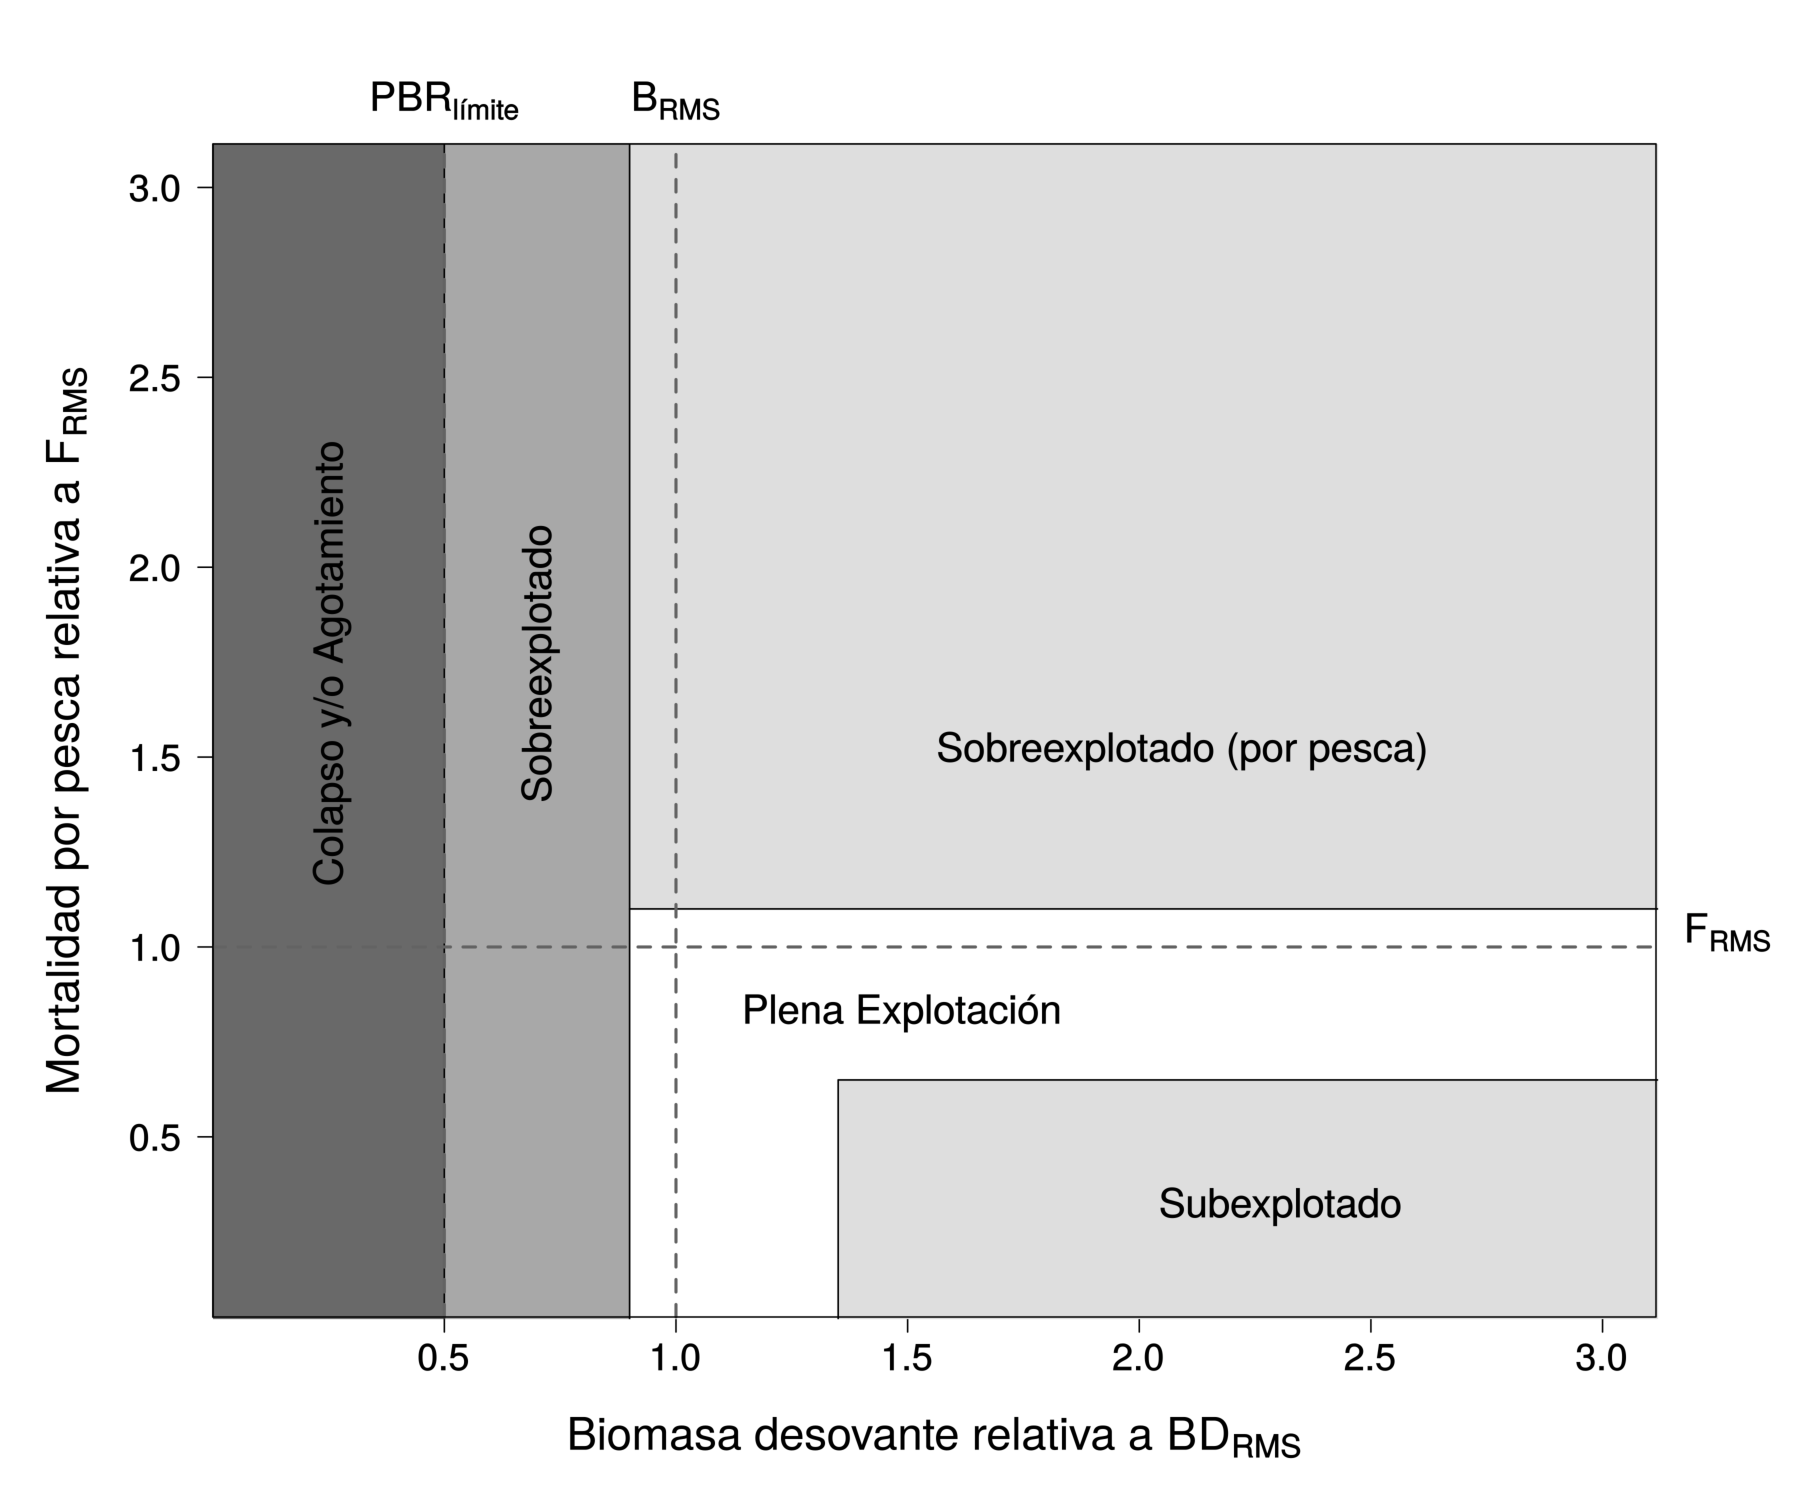
\includegraphics[width=14cm,height=10cm]{Figuras/figura8.pdf}
 \caption{Diagrama de fase tipo para las pesquer\'ias de recursos peque\~{n}os pel\'agicos acordado por el Comit\'e Cient\'ifico T\'ecnico.}
 \label{Fig8}
\end{figure}


\subsubsection{Calidad de la informaci\'on}

Una de las tareas fundamentales en el proceso de evaluaci\'on stock
consiste en dimensionar el nivel de conocimiento del stock en estudio.
Determinar el nivel de calidad de datos e informaci\'on permite definir el
tipo de enfoque de modelamiento que es posible usar para determinar los
niveles poblacionales del stock, as\'i como tambi\'en definir procedimientos
para el c\'alculo de los puntos biol\'ogicos de referencia (PBR). De acuerdo
con Restrepo \textit{et al}. (1998), la calidad de la informaci\'on
permite clasificar el est\'andar de una pesquer\'ia en tres categor\'ias seg\'un
los siguientes criterios:

\textbf{Est\'andar completo (\textquotedblleft Data-Rich\textquotedblright)}: Se pueden realizar
estimaciones confiables del rendimiento m\'aximo sostenido (RMS) y/o de
cantidades relacionadas, as\'i como de la abundancia del stock. La
evaluaci\'on puede ser sofisticada e incorporar la mayor parte de las
fuentes de incertidumbre o bien una cantidad razonable de ella.

\textbf{Est\'andar medio (\textquotedblleft Data-Medium\textquotedblright)}: No se disponen de
estimaciones confiables del rendimiento m\'aximo sostenido y/o cantidades
relacionadas, ya sea porque no est\'an disponibles o bien tienen un uso
limitado debido a peculiaridades de la historia de vida del recurso, a
la pobreza del contraste de los datos, o a la alta variabilidad del
reclutamiento. Sin embargo, existen estimaciones confiables del tama\~{n}o
del stock y de todos los par\'ametros claves de la historia de vida
(crecimiento) y de la pesquer\'ia (selectividad). Este caso se utiliza PBR
gen\'ericos (\textquotedblleft \emph{proxy}\textquotedblright) para sustituir los PBR asociados al RMS que
no se pueden estimar confiablemente.

\textbf{Est\'andar pobre (\textquotedblleft Data-poor\textquotedblright)}: No existen estimados confiables
del rendimiento m\'aximo sostenido, de la abundancia del stock, de los
par\'ametros vitales ni de los par\'ametros de la pesquer\'ia. La evaluaci\'on
es m\'inima y la incertidumbre se aproxima s\'olo cualitativamente. No se
pueden realizar c\'alculos de rendimientos por recluta o biomasas
desovantes por recluta. Este caso se utiliza aproximaciones especiales
para estimar el RMS, tales como \textquotedblleft reglas del pulgar\textquotedblright, promedio de
capturas hist\'oricas corregidas, o m\'as sofisticadas como aproximaciones
bayesianas que usan informaci\'on desde stock con data rica.

El est\'andar de la pesquer\'ia de anchoveta fue revisado a partir de un
listado de t\'opicos generales y espec\'ificos, tomado desde el Anexo D
\textquotedblleft Checklist for the Stock Assessment\textquotedblright (NRC, 1998). Este listado fue
adaptado para las pesquer\'ias chilenas, incluyendo un total de 7 t\'opicos
y 87 preguntas generando la \textquotedblleft matriz de conocimiento\textquotedblright del recurso
(Canales \textit{et al}., 2011). Complementariamente se considera la
asignaci\'on que fue realizada en el marco del proyecto \textquotedblleft Revisi\'on de los
puntos biol\'ogicos de referencia (Rendimiento M\'aximo Sostenible) en las
pesquer\'ias nacionales\textquotedblright realizado por IFOP (Pay\'a \textit{et al}., 2014)
en tres talleres de trabajo y la participaci\'on de 8 expertos
internacionales. \\


\clearpage
\newpage

\subsection{Objetivo espec\'ifico 3.}

\textit{\textquotedblleft Determinar niveles de Captura Biol\'ogicamente Aceptable (CBA) que lleven y/o mantenga la pesquer\'ia en torno al Rendimiento M\'aximo Sostenible (RMS), a partir de un an\'alisis de riesgo en condiciones de incertidumbre de no alcanzar los objetivos de conservaci\'on y sostenibilidad conforme lo establece la LGPA y contenidos en el Plan de Manejo y/o en el Programa de Recuperaci\'on respectivo, seg\'un corresponda.\textquotedblright}
\vspace{0.5cm}

En base al modelo conceptual de la din\'amica del stock respectivo que
sustent\'o el enfoque y modelo de evaluaci\'on aplicado, se realiz\'o un
an\'alisis de la productividad del stock y de sus posibilidades futuras de
explotaci\'on considerando los par\'ametros e indicadores estimados
precedentemente, con su incertidumbre asociada. El an\'alisis considerar\'a
como criterio de explotaci\'on, aquel nivel de mortalidad que conduce al
Rendimiento M\'aximo Sostenido (F$_{RMS}$).

Esta informaci\'on y adem\'as de los antecedentes expuestos ser\'an dados a
conocer a los correspondientes Comit\'es Cient\'ifico T\'ecnicos (CCT) para
que analicen los resultados, considerando los requerimientos de reglas
de decisi\'on establecidas en los Planes de Manejo o programas de
recuperaci\'on respectivos, conforme al marco legal y normativo vigente.
Los an\'alisis consideran entre otros, la proyecci\'on poblacional bajo
condiciones de incertidumbre y la generaci\'on de tablas de decisi\'on sobre
las consecuencias de determinadas acciones en base a posibles estados de
la naturaleza (pesimista, neutro, optimista) de variables de estado
relevantes tales como biomasa desovante y/o niveles de reclutamiento,
junto al riesgo de no lograr determinados objetivos.


\subsubsection{Captura Biol\'ogicamente Aceptable (CBA)}

La estimaci\'on de las capturas biol\'ogicamente aceptables se realiz\'o
mediante un an\'alisis de estrategias de explotaci\'on, que considera
niveles de mortalidad por pesca constante, es decir, las remociones por
pesca son proporcionales a los cambios de abundancia del stock. El
criterio de explotaci\'on est\'a basado en los Puntos Biol\'ogicos de
Referencia (PBR), el cual considera el criterio el F55\%BDPR (biomasa
desovante por recluta) como un proxy del nivel de mortalidad por pesca
que genera el Rendimiento M\'aximo Sostenido (RMS). Adem\'as, es posible
usar otros valores de mortalidad por pesca para realizar estimaciones de
captura y proyecciones del stock.

En el caso de la pesquer\'ia de anchoveta norte, la recomendaci\'on de CBA
comienza con un reporte entregado en el mes de septiembre en que se
estima una CBA inicial. Este reporte permite al CCT-PP (reuni\'on de
octubre) establecer el estatus y recomendar el rango de CBA para el a\~{n}o
siguiente en base a percentiles de riesgo (10\% - 50\%) de sobrepasar el
objetivo de manejo $p(F>F_{RMS})$.\\

\vspace{0.5cm}
\begin{table}[htb!]
 \caption{Informaci\'on relevante para el c\'alculo de CBA 2022 en cada una de las etapas de estimaci\'on.}
 \label{Tab6}
 \centering
 \small
 \begin{tabular}{lcc}
 \hline\noalign{\vskip 0.1cm}
 Datos de entrada & CBA inicial & CBA actualizada \\
 \hline\noalign{\vskip 0.1cm}
 Desembarques Chile & 1986.0 - 2020.5 & 1986.0 - 2021.5 \\
 Desembarques Per\'u & 1986.0 - 2020.5 & 1986.0 - 2021.5 \\
 Descarte Chile & 2017 - 2019.5 & 2017 - 2019.5 \\
 Biomasa ac\'ustica Per\'u & 1990-2020.5 & 1990 - 2021.5 \\
 Biomasa ac\'ustica Chile & 1997-2002, 2007-2020.5 & 1997-2002, 2007-2021.5 \\
 Biomasa desovante Chile (MPDH) & 1992-2020 & 1992-2021.5 \\
 Composici\'on de tallas flota Per\'u & 1986 -2020.5 & 1986 - 2021.5 \\
 Composici\'on de tallas flota Chile & 1986 - 2020.5 & 1986 - 2021.5 \\
 Composici\'on de tallas crucero Chile & 2000-2002 y 2007-2020 & 2000-2002 y 2007-2021 \\
 Pesos medios a la talla Chile & 2001 - 2020.5 & 2001 - 2021.5 \\
 Madurez a la talla Chile & Constante & Constante \\
 Par\'ametros de crecimiento & Constante & Constante \\
 Mortalidad natural & Constante & Constante \\
 Proyecci\'on del reclutamiento & 4 semestres & 2 semestres \\
 \hline
 \end{tabular}
\end{table}

En la sesi\'on de marzo del CCT-PP, con datos actualizados hasta el a\~{n}o
2020 y en base a que el modelo entrega estimaciones de abundancia para
todos los grupos etarios del \'ultimo semestre de evaluaci\'on, entonces se
asumieron los siguientes supuestos para el c\'alculo de la CBA 2021:

\begin{itemize}
\item
  Las proyecciones se realizan en el corto plazo, 2 semestres. (2021.0 y
  2021.5).
\item
  Durante las proyecciones, los reclutamientos a ingresar provienen del
  escenario de reclutamientos promedios diferenciado para el primer y
  segundo semestre (\textbf{Figura \ref{Fig9}}).
\item
  La longitud de la serie de reclutamientos va desde el a\~{n}o 2000 hasta
  el a\~{n}o 2020.
\item
  Durante la proyecci\'on del stock de anchoveta, se consideran los
  niveles de mortalidad por pesca totales ocurridos al \'ultimo semestre
  de la evaluaci\'on, ponderado por la F$_{RMS}$.
\item
  Se asume que los peces capturados es una funci\'on de la poblaci\'on y de
  la mortalidad por pesca y natural (Baranov, 1918).
\item
  La incertidumbre de la CBA se obtendr\'a del error est\'andar de los
  par\'ametros.
\end{itemize}

Para proyectar el stock de anchoveta del sur de Per\'u y norte de Chile es
necesario incorporar los nuevos reclutas para cada semestre proyectado,
primer y segundo semestre del 2021. La elecci\'on de los niveles de
reclutamientos que entran en cada semestre tiene fuertes implicancias en
los niveles poblacionales que se estimen en el futuro y en los niveles
de captura biol\'ogicamente aceptable debido principalmente al r\'apido
crecimiento (\textbf{Figura \ref{Fig3}}) y a una alta mortalidad natural
m\'as la mortalidad por pesca que genera el F$_{RMS}$. Dado que el
\'ultimo reclutamiento estimado por el modelo de evaluaci\'on tiene una alta
incertidumbre, es necesario aplicar el enfoque precautorio en la toma de
decisi\'on inicial sobre los niveles de captura biol\'ogicamente aceptable,
es decir, se podr\'ia considerar el percentil m\'as bajo cuando la
incertidumbre sea alta o penalizar este reclutamiento antes que se
proyecte la poblaci\'on del stock de anchoveta.

\vspace{0.5cm}
\begin{figure}[htb!]
 \centering
 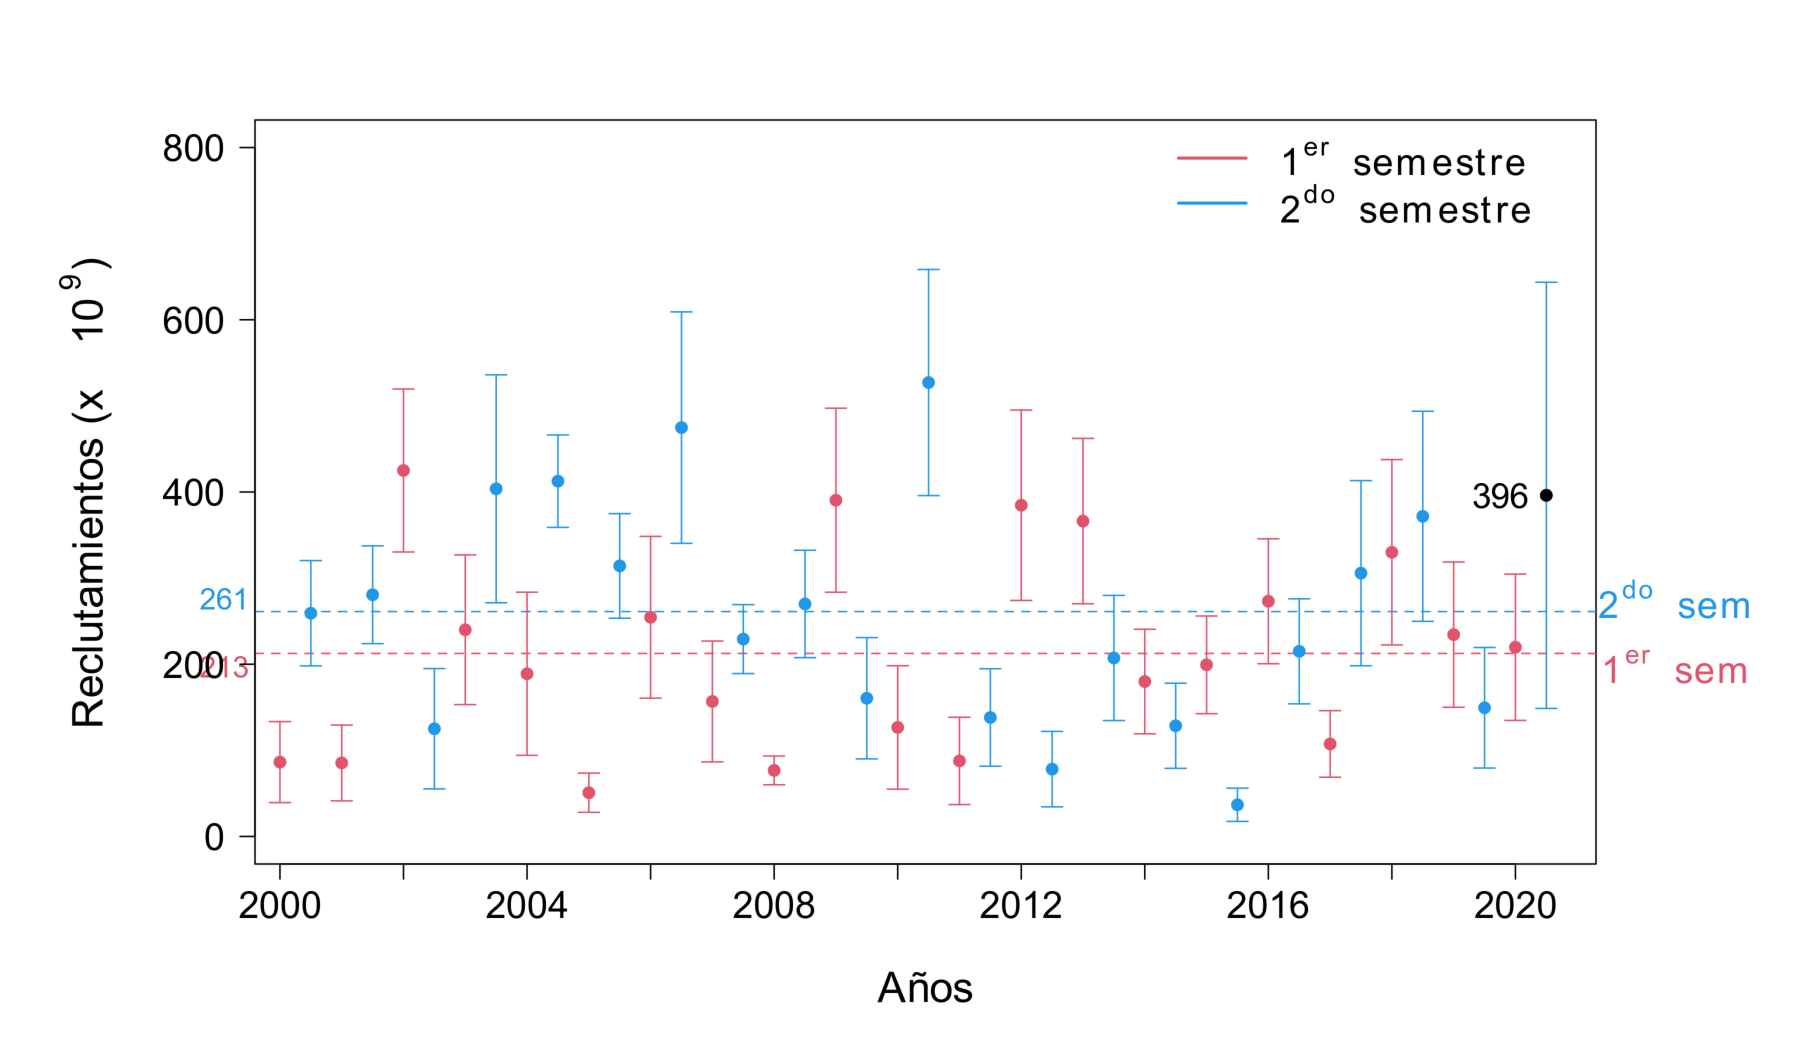
\includegraphics[width=14cm,height=7cm]{Figuras/figura9.pdf}
 \caption{Escenario de reclutamientos promedios diferenciado para el primer y segundo semestre empleados para proyectar el stock de anchoveta del sur de Per\'u y norte de Chile. Las l\'ineas punteadas indican los promedios para cada semestre.}
 \label{Fig9}
\end{figure}

En la actualidad, la CBA considera un rango de valores (de 10 a 50\%)
basado en el riesgo de no alcanzar el objetivo de conservaci\'on. El
riesgo corresponde a una distribuci\'on de probabilidad acumulada y
representa la expectativa de sobrepasar la mortalidad por pesca que
conduce al objetivo de manejo, que es equivalente a mantener el stock
robusto. Dada la alta incertidumbre existente en el establecimiento de
la CBA en el proceso de asesor\'ia inicial, se recomienda utilizar un
nivel de riesgo inferior al 50\%.

En la sexta sesi\'on (octubre del 2019) del CCT-PP se acord\'o una CBA para
el a\~{n}o 2020 de 784,3 mil t con un nivel de riesgo del 30\%. Con el
objeto de mejorar el proceso de establecimiento de CBA y los niveles de
riesgo de no alcanzar el objetivo de manejo, se presenta una propuesta
metodol\'ogica que permite definir un marco de trabajo para la proyecci\'on
poblacional y para la toma de decisi\'on del nivel de riesgo. Seg\'un los
escenarios probables de biomasa de reclutas y/o biomasa desovante del
semestre siguiente al t\'ermino de la evaluaci\'on, y utilizando la
metodolog\'ia indicada por Gruss \textit{et al}. (2016), la cu\'al permite
establecer una CBA mediante la captura al RMS (C$_{RMS}$) y un
porcentaje de resguardo o buffer respecto de la CRMS
(\textbf{Figura \ref{Fig10}}). Este buffer entre la CBA y la captura al
RMS se calcula a partir de la probabilidad de sobrepesca considerada
aceptable (P*) y el error est\'andar de la distribuci\'on de la C$_{RMS}$
(sigma), bajo el supuesto de que la C$_{RMS}$ presenta una
distribuci\'on normal. Dada la distribuci\'on de la C$_{RMS}$, la CBA se
determina de manera que la probabilidad de que CBA exceda C$_{RMS}$
sea igual a P*.

\vspace{0.5cm}
\begin{figure}[htb!]
 \centering
 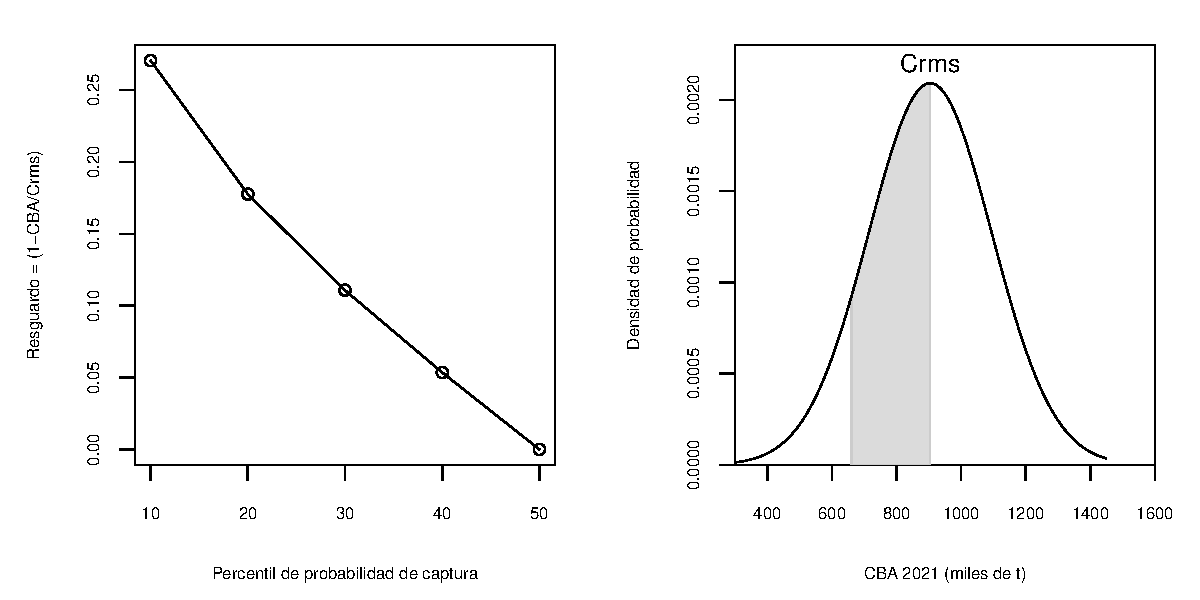
\includegraphics[width=16cm,height=8cm]{Figuras/figura10.pdf}
 \caption{Nivel de resguardo de la Captura al RMS (1-CBA/CRMS) (panel izquierdo) y densidad de probabilidad de la CRMS (panel derecho). La regi\'on sombreada corresponde al rango entre el 10\% - 50\% de probabilidad de sobrepasar la CRMS (P*) que da origen a la CBA determinada por el CCT-PP.}
 \label{Fig10}
\end{figure}


\subsubsection{Incorporaci\'on del descarte en la CBA}

Considerando que el descarte es una fuente de mortalidad adicional a la
mortalidad por pesca, se realiza el descuento a la captura al RMS de un
porcentaje asociado a la captura descartada que podr\'ia ocurrir durante
el primer y segundo semestre del a\~{n}o 2021 en la flota total. Este
supuesto de descarte semestral proyectado se obtiene del promedio de la
serie de datos 2017-2019, correspondiente a un 2\% y un 1,8\% para el
primer y segundo semestre, respectivamente (\textbf{Tabla \ref{Tab7}}).\\

\vspace{0.5cm}
\begin{table}[htb!]
 \caption{Captura total (CT) y descartada (CD) en toneladas promedio 2017-2019 por semestre y flota utilizados para obtener el \% de descarte a utilizar en la proyecci\'on de CBA. Se utiliza la captura total y descartada promedio para la flota total chilena.}
 \label{Tab7}
 \centering
 \small
 \begin{tabular}{cccccc}
 \hline\noalign{\vskip 0.1cm}
 A\~{n}o & Flota & Semestre & CT & CD & \% descarte \\
 \hline\noalign{\vskip 0.1cm}
 \multirow{2}{*}{2021} &\multirow{2}{*}{Total} & 1 & 501.860 & 10.054 & 2.0 \\
 & & 2 & 229.877 & 4.150 & 1,8 \\
 \hline
 \end{tabular}
\end{table}


\subsubsection{Proyecci\'on del stock}

Finalmente, se realiza un conjunto de an\'alisis estoc\'asticos de las
probables trayectorias de la biomasa desovante como consecuencia de la
aplicaci\'on de las diferentes estrategias, t\'acticas y reglas de decisi\'on
consideradas en los respectivos Planes de Manejo y/o Programas de
Recuperaci\'on de las pesquer\'ias, seg\'un corresponda, considerando la
incertidumbre del estatus (e.g. matriz de correlaci\'on de variables de
estado) y los posibles estados de la naturaleza a futuro (e.g. niveles
probables de reclutamiento futuro). Lo anterior debe permitir analizar
los niveles de riesgo de no alcanzar los objetivos de conservaci\'on en el
corto o mediano plazo, considerando la incertidumbre del estatus y los
probables estados de la naturaleza a futuro.\\


\clearpage
\newpage

\subsection{Objetivo espec\'ifico 4.}

\textit{\textquotedblleft Informar el avance del Programa de Mejoramiento Continuo de la Calidad en la Asesor\'ia Cient\'ifica (PMCCAC) realizado durante el presente estudio, respecto al cumplimiento de recomendaciones formuladas en procesos de RPEI y priorizadas por el CCT, cuando corresponda.\textquotedblright}
\vspace{-0.2cm}

\subsubsection{Programa de mejoramiento continuo de la calidad de la asesor\'ia cient\'ifica}

Para el cumplimiento de este objetivo, se informar\'a de los avances
alcanzados durante el desarrollo del estudio, conforme al Programa de
Mejoramiento Continuo de la Calidad de la Asesor\'ia Cient\'ifica (PMCCAC),
elaborado por recurso y/o pesquer\'ia. Este PMCCAC se enfocar\'a a las
brechas de datos, informaci\'on y conocimiento, en relaci\'on con la
situaci\'on general de la pesquer\'ia acorde con los requerimientos de
asesor\'ia solicitados por la administraci\'on pesquera. Sobre la base de lo
anterior, se evaluar\'a el desempe\~{n}o logrado y se propondr\'an las acciones,
actividades, metas, plazos y condiciones que consideren necesarios para
lograr disminuir las brechas identificadas y los requerimientos para
alcanzar los est\'andares de asesor\'ia previamente definidos.

En el contexto del desarrollo metodol\'ogico del trabajo, se realizar\'a un
listado de comprobaci\'on en el que se deber\'a dar cuenta de todas las
recomendaciones emanadas de los revisores expertos, con el prop\'osito de
verificar el cumplimiento de cada uno de las observaciones, correcciones
y recomendaciones se\~{n}aladas por los revisores.

En el caso de aquellos recursos cuyas metodolog\'ias de evaluaci\'on de
stock hayan sido sometidas a Procesos de Revisi\'on por Pares (PRPP), el
informe deber\'a contener una secci\'on especialmente dedicada a informar
detalladamente c\'omo se abordaron y fueron implementadas cada una de las
recomendaciones realizadas por los expertos revisores externos (e. g.,
situaci\'on anterior, modificaci\'on, situaci\'on post- revisi\'on con los
cambios/mejoras implementadas), a la forma de un listado de comprobaci\'on
(o checklist).

\emph{Actividades}

\begin{itemize}
\def\labelenumi{\roman{enumi})}
\item
  Ejecuci\'on de un programa de trabajo.
\item
  Elaboraci\'on de un informe conteniendo los avances y resultados durante
  el periodo anual del proyecto, conteniendo el PMCCAC actualizado y un
  listado de comprobaci\\on (inicio/final) de sus logros.
\item
  Para aquellas pesquer\'ias que se han sometido a revisi\'on de pares,
  elaborar un informe detallado respecto del avance en la incorporaci\'on
  de las recomendaciones de los expertos.
\end{itemize}


\clearpage
\newpage

\section{RESULTADOS}


\subsection{Objetivo espec\'ifico 1.}

\textit{\textquotedblleft Implementar procedimientos de evaluaci\'on de stock basados en protocolos cient\'ificos para la determinaci\'on del estatus de anchoveta y sardina espa\~{n}ola, con arreglo al nivel de informaci\'on, conocimiento e incertidumbre correspondiente, conforme a los est\'andares actuales en ciencia pesquera.\textquotedblright}
\vspace{0.5cm}


\subsubsection{Datos de entrada al modelo de evaluaci\'on de stock}

El periodo de an\'alisis de la evaluaci\'on de stock comienza en 1986 hasta
el segundo semestre del 2020, con informaci\'on completa hasta el segundo
semestre del a\~{n}o 2020. Se incluye la biomasa total y composici\'on de la
estructura de tama\~{n}os estimada por el crucero de Chile, la biomasa total
del sur de Per\'u, la biomasa desovante estimada por el MPH en Chile, la
composici\'on de la estructura de tama\~{n}os y el desembarque para la flota
chilena. No as\'i la flota peruana, que no registro capturas durante el
a\~{n}o 2020.


\paragraph{a) Desembarques}

\quad

La historia de la pesquer\'ia del stock de anchoveta compartido entre el
sur de Per\'u y norte de Chile, comienza con leves desembarques ocurridos
en 1984 y a contar de 1986 se incrementan considerablemente hasta el a\~{n}o
1994 (\textbf{Tabla \ref{Tab8}}; \textbf{Figura \ref{Fig11}}), los m\'as
altos desembarques ocurren entre los a\~{n}os 1994 al 2002. Desde el a\~{n}o
2004 al primer semestre 2013 estos muestran una tendencia de descenso
con m\'aximos relativos. El desembarque por pa\'is muestra un cambio de
dominancia. Entre los a\~{n}os 1986 al 2004 se puede se\~{n}alar que el mayor
desembarque fue realizado en Chile. Sin embargo, entre el 2005 al 2009
los mayores desembarques se realizaron en Per\'u. Entre las causas
probables de la dominancia peruana del desembarque se encuentra el
aumento del esfuerzo de pesca en la pesquer\'ia del sur del Per\'u debido a
la mayor disponibilidad de anchoveta en dicha \'area seg\'un lo informado
por IMARPE en el 12$^{do}$ taller de evaluaci\'on conjunta de IFOP e IMARPE,
2008 (Serra y Canales, 2013). Y desde el a\~{n}o 2010 a diciembre del 2013
el desembarque chileno ha dominado el desembarque total del stock
anchoveta. Se postula que el incremento del desembarque chileno en el
a\~{n}o 2011 habr\'ia estado asociado a un desplazamiento de la anchoveta del
sur de Per\'u hacia el norte de Chile evidenci\'andose un incremento del
desembarque particularmente en la zona de Arica (B\"ohm \textit{et al}.,
2013).

M\'as recientemente y de acuerdo a las estad\'isticas oficiales, el primer y
segundo semestre del 2014 se capturaron en Chile 375.1 mil y 354.3 mil
toneladas, respectivamente. Por su parte, en el sur del Per\'u y de
acuerdo a lo informado en Oficio PRODUCE 100-59-2015, el desembarque
acumulado de enero a octubre hab\'ia sido de 336.7 mil toneladas, de las
cuales solo 26 mil toneladas fueron capturadas en el segundo semestre.
Si se considera adem\'as que producto de este oficio la captura de
anchoveta fue prohibida en la zona sur del Per\'u en noviembre y diciembre
2014 debido a la gran presencia de reclutas, se deduce entonces que la
captura en esta regi\'on pudo haber alcanzado 310 mil toneladas durante el
primer semestre del 2014. De esta forma, el desembarque total 2014 se
estima en 1.082 millones de toneladas (\textbf{Tabla \ref{Tab8}}) el
cual se traduce un alza del 15\% respecto del a\~{n}o 2013, y el desembarque
del 2015 disminuy\'o en un 1\% con respecto al 2013. Y el desembarque del
2015 se tradujo en una disminuci\'on del 14\% con respecto al del 2014.
Sin embargo, el desembarque durante el 2016 se redujo fuertemente,
alcanzando 397 mil toneladas para ambos pa\'ises. Y finalmente, en el a\~{n}o
2017 el desembarque aumento a 708 mil toneladas. Cerrando el a\~{n}o 2018,
se registra un desembarque total de 971.1 mil toneladas, un 37\%
superior a lo registrado en el 2017. Desde el 2016 hasta el 2018 se
viene registrando un aumento constante de los desembarques, pasando de
397.4, 708.7, 984.1 mil toneladas, respectivamente
(\textbf{Figura \ref{Fig11}}). Desde el 2019 hasta el 2020 se registra
una disminuci\'on del desembarque, pasando desde 719.9 a 271.9 mil
toneladas, un reducci\'on del 62\%. \\

\newpage

\vspace{0.5cm}
\begin{table}[htb!]
 \caption{Desembarques del stock de anchoveta 16\degree - 24\degree LS 1986-2020.}
 \label{Tab8}
 \centering
 \small
 \begin{tabular}{cccc}
 \hline\noalign{\vskip 0.1cm}
 A\~{n}o & Sur Per\'u & Norte Chile & Total \\
 \hline\noalign{\vskip 0.1cm}
 1986  &  321.2  &  1248.7  &  1560.9  \\
 1987  &  246.4  &   178.8  &   425.2  \\
 1988  &  285.6  &   768.5  &  1054.1  \\
 1989  &  462.8  &  1263.8  &  1726.6  \\
 1990  &  179.9  &   573.1  &   753.0  \\
 1991  &  377.5  &   562.8  &   940.3  \\
 1992  &  873.2  &   953.9  &  1827.1  \\
 1993  &  631.4  &  1056.2  &  1687.1  \\
 1994  &  849.2  &  1945.0  &  2794.2  \\
 1995  &  971.5  &  1482.1  &  2453.6  \\
 1996  &  183.8  &   840.0  &  1023.8  \\
 1997  & 1080.6  &  1317.4  &  2398.0  \\  
 1998  &  297.0  &   132.7  &   429.7  \\
 1999  &  539.4  &   809.2  &  1348.6  \\
 2000  &  483.8  &  1154.4  &  1638.2  \\
 2001  &  360.8  &   639.8  &  1000.6  \\
 2002  & 1341.6  &  1216.0  &  2557.6  \\
 2003  &  193.7  &   417.9  &   611.6  \\
 2004  &  882.8  &  1394.1  &  2276.9  \\
 2005  & 1037.9  &  1007.7  &  2045.6  \\
 2006  &  819.8  &   513.1  &  1332.9  \\
 2007  &  943.4  &   744.8  &  1688.2  \\
 2008  &  846.8  &   648.2  &  1495.0  \\
 2009  &  541.3  &   440.2  &   981.5  \\
 2010  &  290.5  &   435.0  &   725.5  \\
 2011  &  546.8  &   958.0  &  1504.8  \\
 2012  &  272.9  &   710.1  &   983.0  \\
 2013  &  246.0  &   691.0  &   937.0  \\
 2014  &  353.0  &   729.4  &  1082.4  \\
 2015  &  293.0  &   633.0  &   926.0  \\
 2016  &  154.0  &   243.4  &   397.4  \\
 2017  &  179.0  &   529.7  &   708.7  \\
 2018  &  220.0  &   751.1  &   971.1  \\
 2019  &  195.0  &   524.9  &   719.9  \\
 2020  &  \---   &   271.9  &   271.9  \\
 \hline
 \end{tabular}
\end{table}

\vspace{0.5cm}
\vspace{0.5cm}
\begin{figure}[htb!]
 \centering
 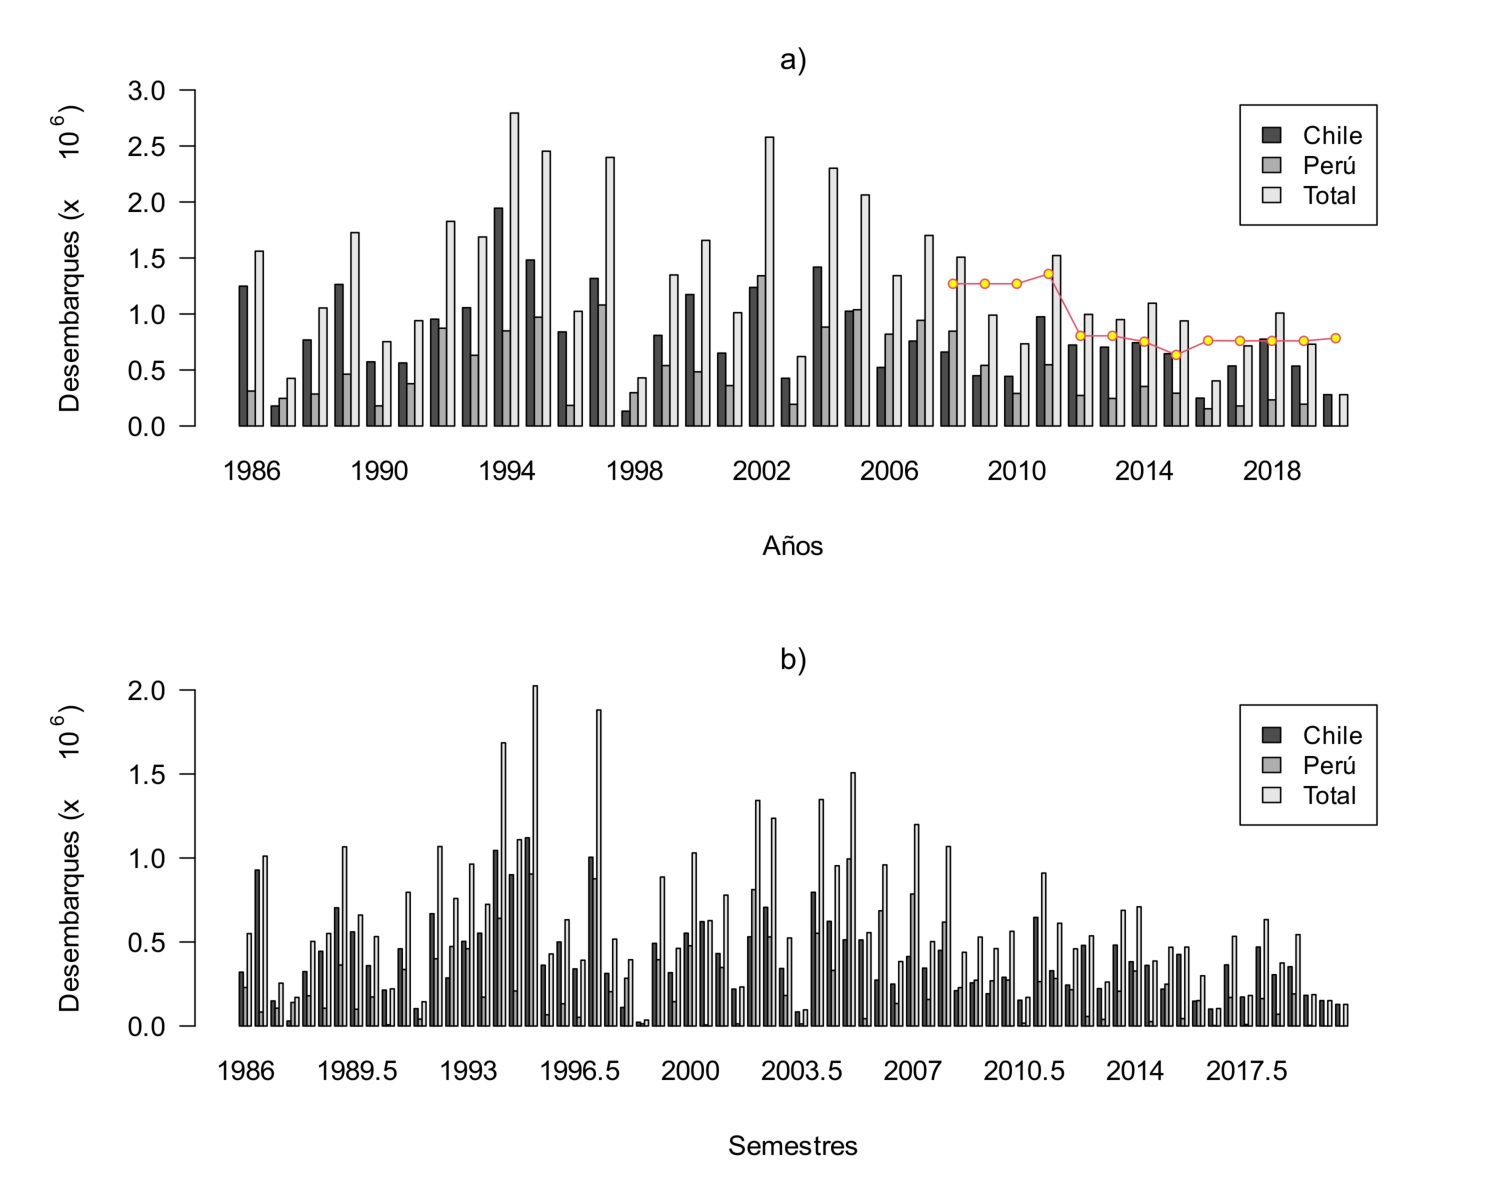
\includegraphics[width=17cm,height=10cm]{Figuras/figura11.pdf}
 \caption{Desembarques anuales y semestrales para Chile, Per\'u y Total del stock de anchoveta distribuido entre 16\degree LS - 24\degree LS (1986 - 2020). Los puntos amarillos representan la cuota chilena. En el panel superior (a) se muestra el desembarque en escala anual y en el panel inferior (b) en escala semestral.}
 \label{Fig11}
\end{figure}


\paragraph{b) Descarte}

\quad

La evaluaci\'on de stock de anchoveta norte incorpora los porcentajes de
descarte estimados entre el 2017 al 2019 (\textbf{Tabla \ref{Tab2}} y
\textbf{Tabla \ref{Tab3}}) para corregir la serie de desembarques
semestrales de la flota chilena artesanal e industrial de anchoveta
norte. Los supuestos de descarte utilizados en la evaluaci\'on de stock
entregada en la asesor\'ia de marzo 2021 (2$^{do}$ Hito CBA 2021) fueron los
siguientes:

\begin{itemize}
\item El supuesto 1 de descarte propuesto para la correcci\'on de la serie de desembarques semestrales (2020.0, 2020.5) para flota artesanal e industrial se obtiene del promedio de serie 2017-2019.
\item El supuesto 2 de descarte propuesto para la proyecci\'on de la CBA semestral 2021 para la flota total se obtiene del promedio de la serie de datos 2017-2019.
\end{itemize}

El supuesto 1 se justifica debido a la alta incertidumbre de la
estimaci\'on de captura descartada del primer semestre 2020 por las
siguientes razones:

\begin{itemize}
\item Se prohiben perforaciones de la flota industrial.
\item S\'olo captura anchoveta flota artesanal.
\item Flota industrial redirige su esfuerzo a captura de jurel (baja captura de anchoveta).
\item Disminuyen el n\'umero de viajes muestreados por protocoles de seguridad (pandemia).
\item Baja cobertura de muestreo.
\end{itemize}

Los supuestos sugeridos para la asesor\'ia de septiembre 2021 (1$^{er}$ Hito
CBA 2022) son los siguientes:

\begin{itemize}
\item El supuesto 1 de descarte propuesto para la correcci\'on de la serie de desembarques semestrales (2020.0) para flota artesanal e industrial se obtiene del promedio de serie 2017-2019. Se sugiere revisar el supuesto de descarte del Segundo semestre del 2020 (2020.5) con informaci\'on actualizada del descarte.
\item El supuesto 2 de descarte propuesto para la proyecci\'on de la CBA semestral 2021 y 2022 para la flota total se obtiene del promedio de la serie de datos 2017-2019.
\end{itemize}

El IFOP present\'o al CCT-PP, en la sesi\'on de febrero de 2021, un resumen
de las estimaciones de descarte y una propuesta de un procedimiento
est\'andar a implementar por un plazo de dos a\~{n}os, como mecanismo
transitorio para compensar la incertidumbre de las estimaciones del
descarte usado como input en la determinaci\'on de la CBA. El Comit\'e
acuerda aplicar a la CBA m\'axima de la anchoveta norte, un valor de
descarte del 2\% para el primer semestre y un 1.8\% en el segundo
semestre, durante el 2020 y 2021
(\href{http://www.subpesca.cl/portal/616/articles-110238_documento.pdf}).


\paragraph{c) Composici\'on de longitud de la captura y cruceros}

\quad

El n\'umero de individuos pescados a la talla en las capturas totales
(COLOCAP) se elabora en base mensual tanto de la pesquer\'ia del sur de
Per\'u como del norte de Chile. En Per\'u la expansi\'on de las tallas a las
capturas se realiza en base diaria y por puerto, en la pesquer\'ia del
norte de Chile se realiza en base mensual y por macrozona hasta el 2007.
Desde el 2008 se construyen por viaje dentro de cada macrozona, donde
las composiciones de tallas muestrales son ponderadas por las capturas.
Las macrozonas son:

\begin{itemize}
\item
  Arica: L\'imite -- 19\degree 30'LS
\item
  Iquique: 19\degree 30'LS -- 21\degree 30'LS
\item
  Antofagasta: 21\degree 30'LS -- 24\degree 00'LS
\end{itemize}

Para la pesquer\'ia chilena cubren el periodo comprendido entre el primer
semestre de 1986 y el segundo semestre 2020, mientras que la pesquer\'ia
peruana incorpora informaci\'on hasta el segundo semestre del 2019. Los
COLOCAP semestrales de ambas pesquer\'ias muestran diferencias que
justifican el uso de un modelo que discrimine por flotas.Por ejemplo,
desde el 2002 y hasta el 2011, la flota peruana captur\'o sistem\'aticamente
ejemplares de menor tama\~{n}o que los registrados en el norte de Chile. En
general, las tallas han disminuido fuertemente en ambas pesquer\'ias,
alcanzando valores medios en torno a los 11 cm de LT en el a\~{n}o 2019
(\textbf{Figura \ref{Fig12}}).

\vspace{0.5cm}
\begin{figure}[htb!]
 \centering
 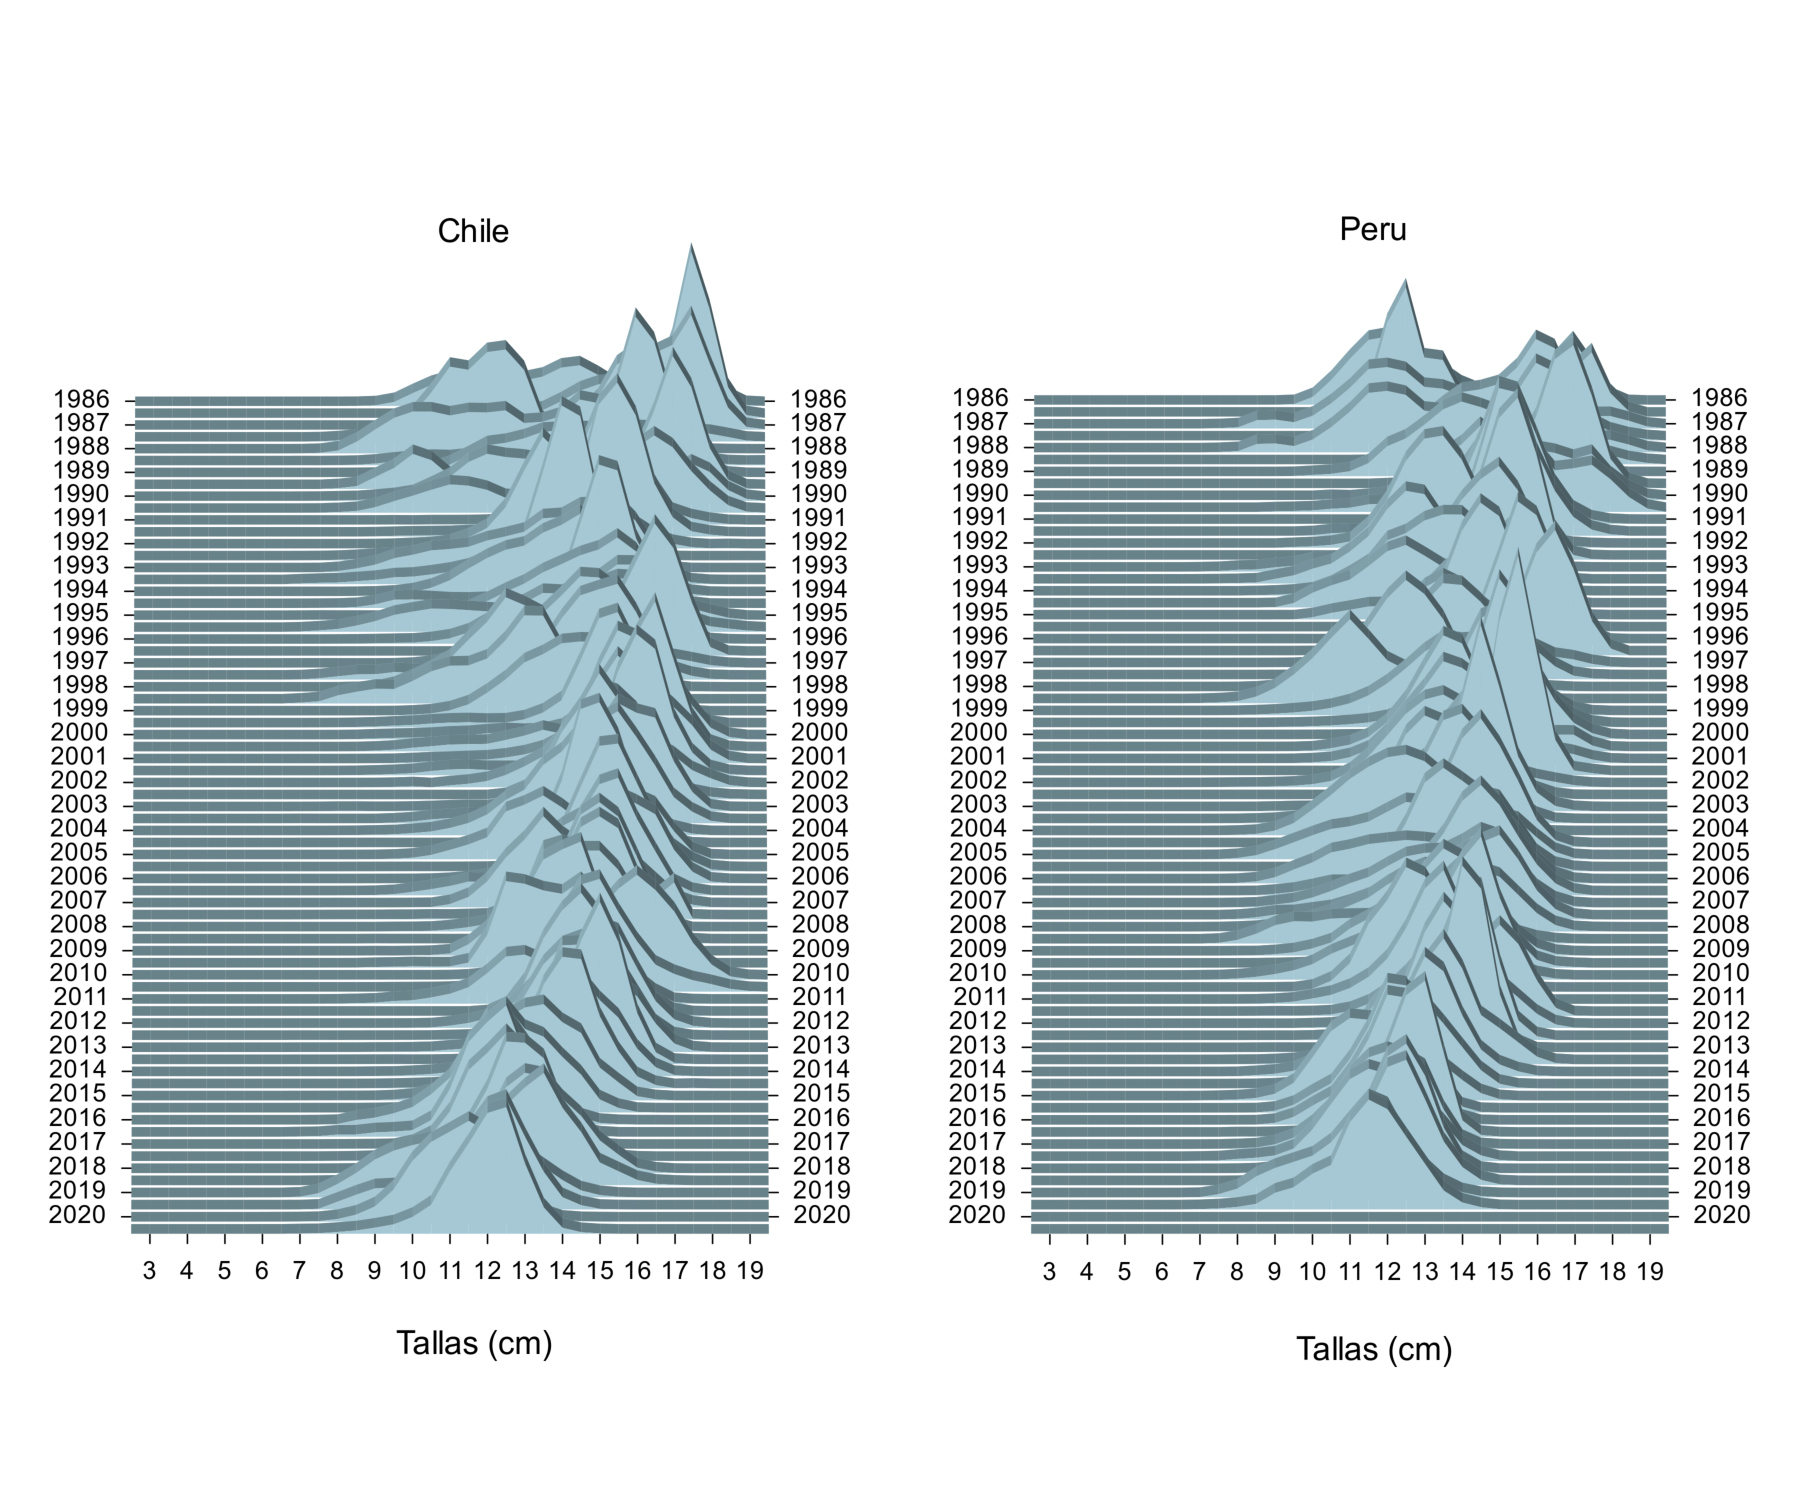
\includegraphics[width=19cm,height=12cm]{Figuras/figura12.pdf}
 \caption{Proporci\'on por tallas de las capturas semestrales en las pesquer\'ias de anchoveta del sur de Per\'u y norte de Chile (1986 – 2020).}
 \label{Fig12}
\end{figure}

Adem\'as, para la pesquer\'ia chilena se analizan los datos de los muestreos
biol\'ogicos efectuados por el programa de seguimiento de la pesquer\'ia
desarrollado por IFOP y los resultados muestran la proporci\'on en la
captura de cuatro categor\'ias de tallas a desde el 2001 hasta el 2020
(\textbf{Figura \ref{Fig13}}). Desde el 2001 hay una predominancia de
individuos de 14 a 16 cm de longitud y una baja incidencia de individuos
de 12 a 13.5 cm, alcanzando sobre el 40\% en el 2004 y 2007. Desde del
2007 en adelante este porcentaje aumenta considerablemente y se observa
en una mayor frecuencia, llegando alcanzar valores por sobre el 80\% en
el 2011. Desde el 2015 dominan gran parte de la serie y se observa una
participaci\'on significativa de individuos menores a los 11.5 cm de
longitud. Durante el 2020 dominan las tallas de 12 a 13.5 cm de
longitud, con una alta participaci\'on de tallas menores a los 11.5 cm.
Esta tendencia en la disminuci\'on de las tallas durante los \'ultimos a\~{n}os
tambi\'en es apreciable en la talla media (\textbf{Figura \ref{Fig14}}),
que desde el 2014 registra una disminuci\'on hasta alcanzar los 10 cm a
comienzos del 2016. Luego, se mantiene entre los 12 a 14 cm para
nuevamente disminuir hasta los 10 cm en el 2019. Hacia el final del 2019
y durante el 2020 se registr\'o una talla media en torno a los 12 cm.

\vspace{0.5cm}
\begin{figure}[htb!]
 \centering
 \includegraphics[width=16.5cm,height=12cm]{Figuras/figura13.pdf}
 \caption{Participaci\'on de las tallas en las capturas de la flota chilena por intervalo de talla desde el 2001 hasta el 2019. El color azul ($>$16.5 cm), color verde (14 a 16 cm), color rojo (12 a 13.5 cm) y color negro ($<=$11.5 cm).}
 \label{Fig13}
\end{figure}

\vspace{0.5cm}
\begin{figure}[htb!]
 \centering
 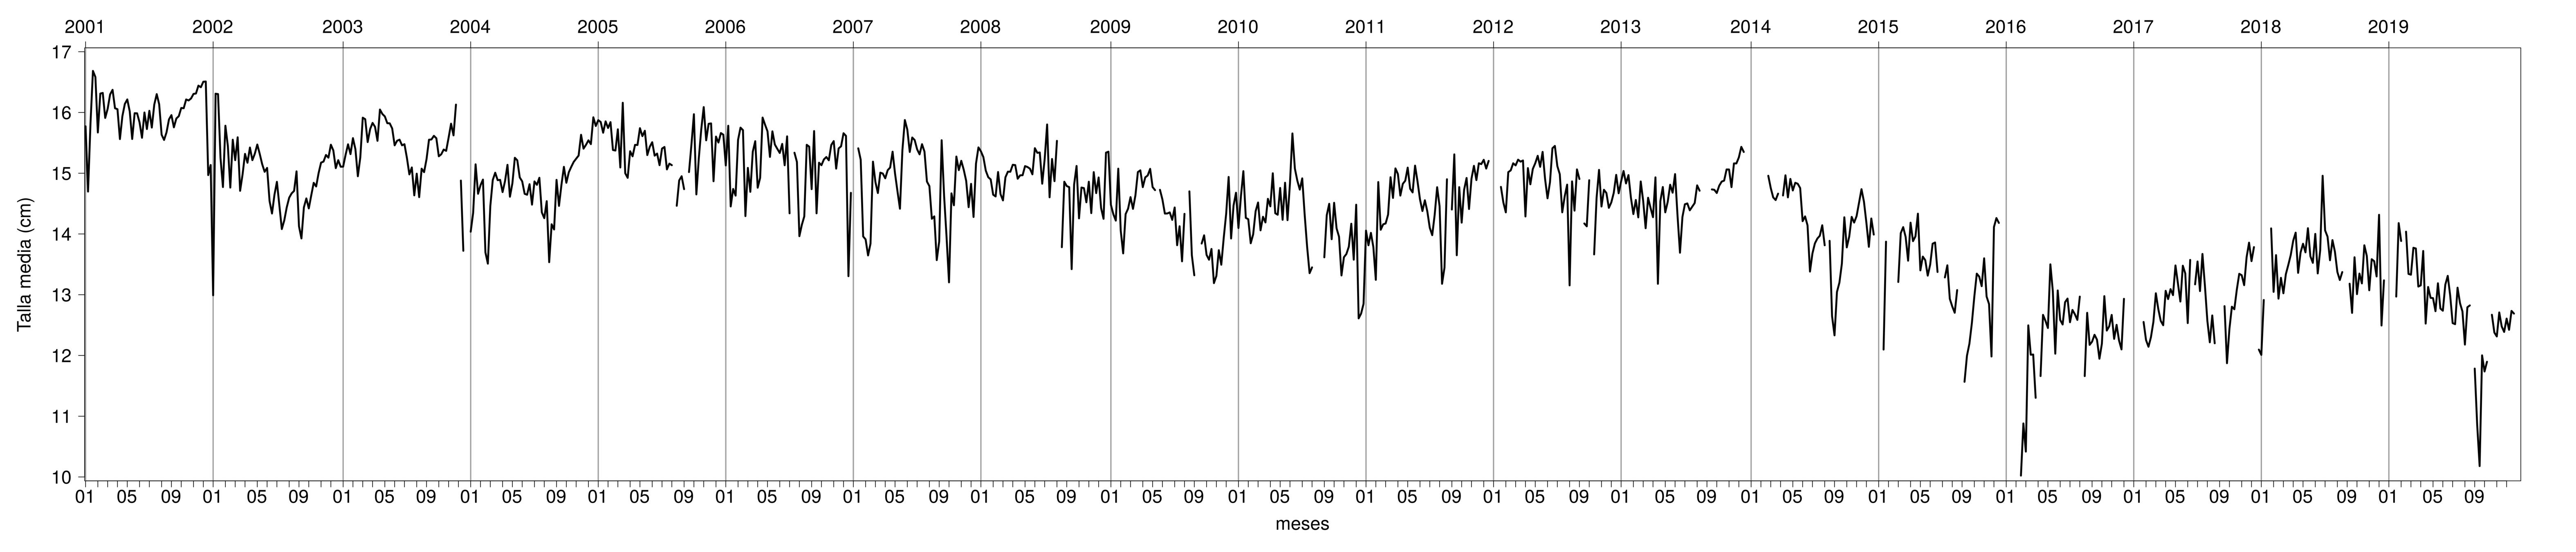
\includegraphics[width=16.5cm,height=12cm]{Figuras/figura14.pdf}
 \caption{Serie temporal de la talla media en las capturas de la flota chilena desde el 2001 hasta el 2020.}
 \label{Fig14}
\end{figure}


\paragraph{d) Pesos y madurez a la talla}

\quad

Entre los a\~{n}os 1986 y 2000 se utiliza un valor de peso medio a la talla
obtenido desde los par\'ametros de la relaci\'on longitud-peso para el
mismo periodo (promedio) en la zona norte de Chile (XV-II Regiones). Los
coeficientes de la relaci\'on son: a= 0.00625 y b= 3.02561. Y para los
a\~{n}os 2001 hasta 2020 se utiliza una relaci\'on longitud-peso variable por
semestre ajustada mediante modelos no lineales mixtos (Pinheiro y Bates,
2000), en que los par\'ametros a y b de la relaci\'on longitud-peso son
considerados como efectos aleatorios (\textbf{Tabla \ref{Tab9}} y
\textbf{Figura \ref{Fig15}}). En cuanto a la madurez, se utiliza la
ojiva a la talla obtenida por Mart\'inez \textit{et al}. (2009), cuya
talla media de madurez corresponde a 11.5 cm en longitud total. La
funci\'on de proporci\'on de individuos maduros a la talla se muestra en la
\textbf{Figura \ref{Fig16}}.

\vspace{0.5cm}
\begin{figure}[htb!]
 \centering
 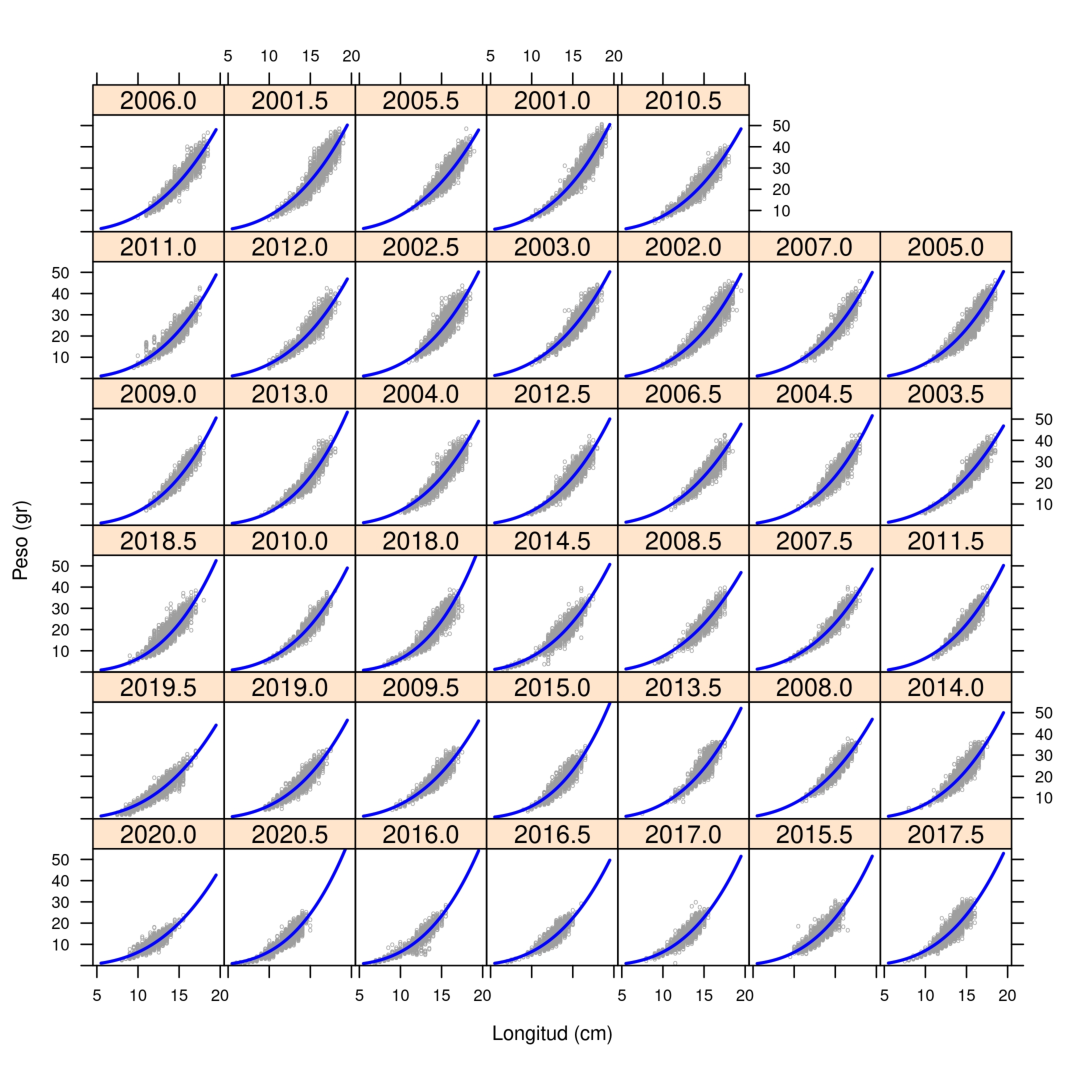
\includegraphics[width=13cm,height=11cm]{Figuras/figura15.pdf}
 \caption{Relaci\'on longitud-peso variable por semestres desde el 2001 hasta el 2020. Cada curva (l\'inea azul) fue ajustada por medio de modelos mixtos con efectos aleatorios.}
 \label{Fig15}
\end{figure}

\newpage

\vspace{0.5cm}
\begin{table}[htb!]
 \caption{Par\'ametros \textit{a} y \textit{b} de la relaci\'on longitud-peso estimados por modelo no lineales mixtos.}
 \label{Tab9}
 \centering
 \small
 \begin{tabular}{ccc}
 \hline\noalign{\vskip 0.1cm}
 Semestre & \textit{a} & \textit{b} \\
 \hline\noalign{\vskip 0.1cm}
 2001.0 & 0.007810934 & 2.953925 \\
 2001.5 & 0.011107999 & 2.833511 \\
 2002.0 & 0.006689012 & 2.996512 \\
 2002.5 & 0.007180881 & 2.980155 \\
 2003.0 & 0.011145474 & 2.832652 \\
 2003.5 & 0.012501097 & 2.769733 \\
 2004.0 & 0.008088254 & 2.931933 \\
 2004.5 & 0.005530761 & 3.077420 \\
 2005.0 & 0.008281394 & 2.931933 \\
 2005.5 & 0.014549947 & 2.726752 \\
 2006.0 & 0.013851617 & 2.744509 \\
 2006.5 & 0.012773019 & 2.768485 \\
 2007.0 & 0.007564375 & 2.961119 \\
 2007.5 & 0.010773553 & 2.832238 \\
 2008.0 & 0.011974593 & 2.785081 \\
 2008.5 & 0.012830483 & 2.761722 \\
 2009.0 & 0.005619524 & 3.065078 \\
 2009.5 & 0.009529009 & 2.856279 \\
 2010.0 & 0.005298669 & 3.074377 \\
 2010.5 & 0.011398358 & 2.812732 \\
 2011.0 & 0.007784679 & 2.943700 \\
 2011.5 & 0.005732487 & 3.056045 \\
 2012.0 & 0.008782683 & 2.889336 \\
 2012.5 & 0.006577518 & 3.008842 \\
 2013.0 & 0.003655199 & 3.227376 \\
 2013.5 & 0.007650149 & 2.994775 \\
 2014.0 & 0.007650149 & 2.957364 \\
 2014.5 & 0.008815520 & 2.914416 \\
 2015.0 & 0.002972675 & 3.303684 \\
 2015.5 & 0.004319944 & 3.160051 \\
 2016.0 & 0.004162371 & 3.188746 \\
 2016.5 & 0.005994121 & 3.037969 \\
 2017.0 & 0.004849688 & 3.120800 \\
 2017.5 & 0.006904577 & 3.010688 \\
 2018.0 & 0.002855162 & 3.338865 \\
 2018.5 & 0.004324776 & 3.165825 \\
 2019.0 & 0.005989567 & 3.015624 \\
 2019.5 & 0.011380066 & 2.781900 \\
 2020.0 & 0.008502352 & 2.868338 \\
 2020.5 & 0.003946365 & 3.224859 \\
 \hline
 \end{tabular}
\end{table}

\vspace{0.5cm}
\begin{figure}[htb!]
 \centering
 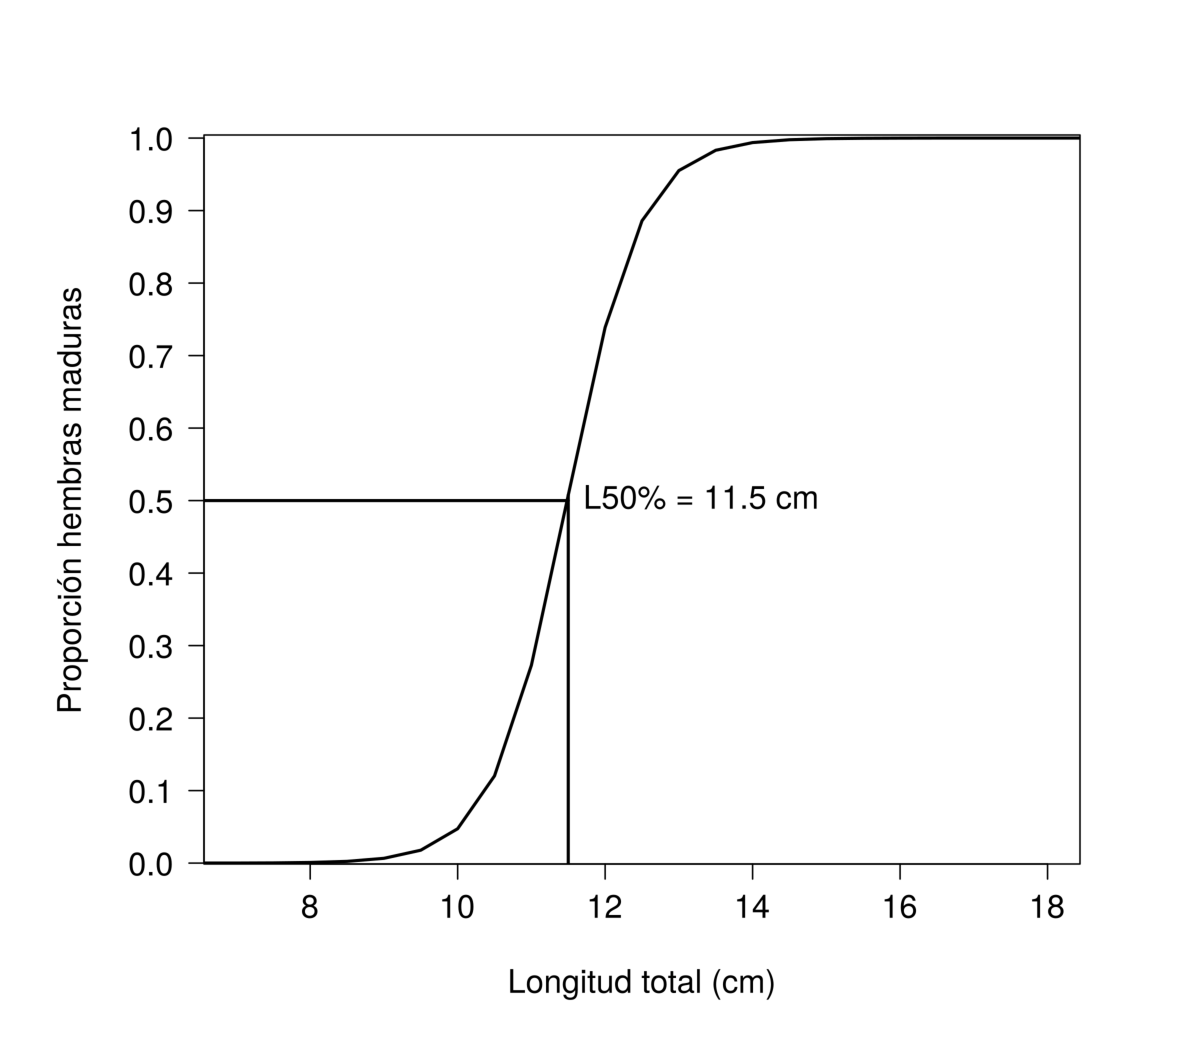
\includegraphics[width=11cm,height=9cm]{Figuras/figura16.pdf}
 \caption{Ojiva de madurez sexual a la talla para la anchoveta obtenida de Mart\'inez \textit{et al}. (2009).}
 \label{Fig16}
\end{figure}


\paragraph{e) Crecimiento}

\quad

Como fue mencionado en el \textbf{Punto 2.6}, en relaci\'on de los nuevos
antecedentes sobre el crecimiento de la anchoveta del norte de Chile
(Plaza \textit{et al}., 2017), se\~{n}alan una din\'amica m\'as r\'apida que la
establecida para las especies de \textit{Engraulis} de otros ecosistemas
de surgencia de borde oriental tales como Butler (1989), Waldron
\textit{et al}. (1989 y 1992), Melo (1984) y Prosch (1986). Estos
resultados se\~{n}alan un coeficiente de crecimiento de $k$ = 1.96
a\~{n}o$^{-1}$, $t_0$ = 0.013 a\~{n}o y $L_{inf}$ = 19.85 cm.
\vspace{0.5cm}

Sin embargo, durante el Taller Benchmark realizado en julio del 2019 se
revisaron los diferentes casos de crecimiento, tanto los que incorporan
la estacionalidad en el crecimiento como aquellos basados en el modelo
de von Bertalanffy tradicional. Los resultados indican que el modelo
tradicional de von Bertalanffy no difiere mucho de los modelos
estacionales (\textbf{Figura \ref{Fig17}}) y que el modelo tradicional
de crecimiento fue el que mejor se ajust\'o a los datos de la evaluaci\'on
durante el Taller Benchmark (\textbf{Tabla \ref{Tab10}}). \vspace{0.5cm}

\vspace{0.5cm}
\begin{table}[htb!]
 \caption{Par\'ametros de crecimiento estimados del modelo de von Bertalanffy.}
 \label{Tab10}
 \centering
 \small
 \begin{tabular}{ccc}
 \hline\noalign{\vskip 0.1cm}
 $t_0$ (a\~{n}o) & $k$ (a\~{n}o$^{-1}$) & $L_{inf}$ (cm) \\
 \hline\noalign{\vskip 0.1cm}
 0.01 & 2.12 & 17.55 \\
 \hline
 \end{tabular}
\end{table}

\vspace{0.5cm}
\begin{figure}[htb!]
 \centering
 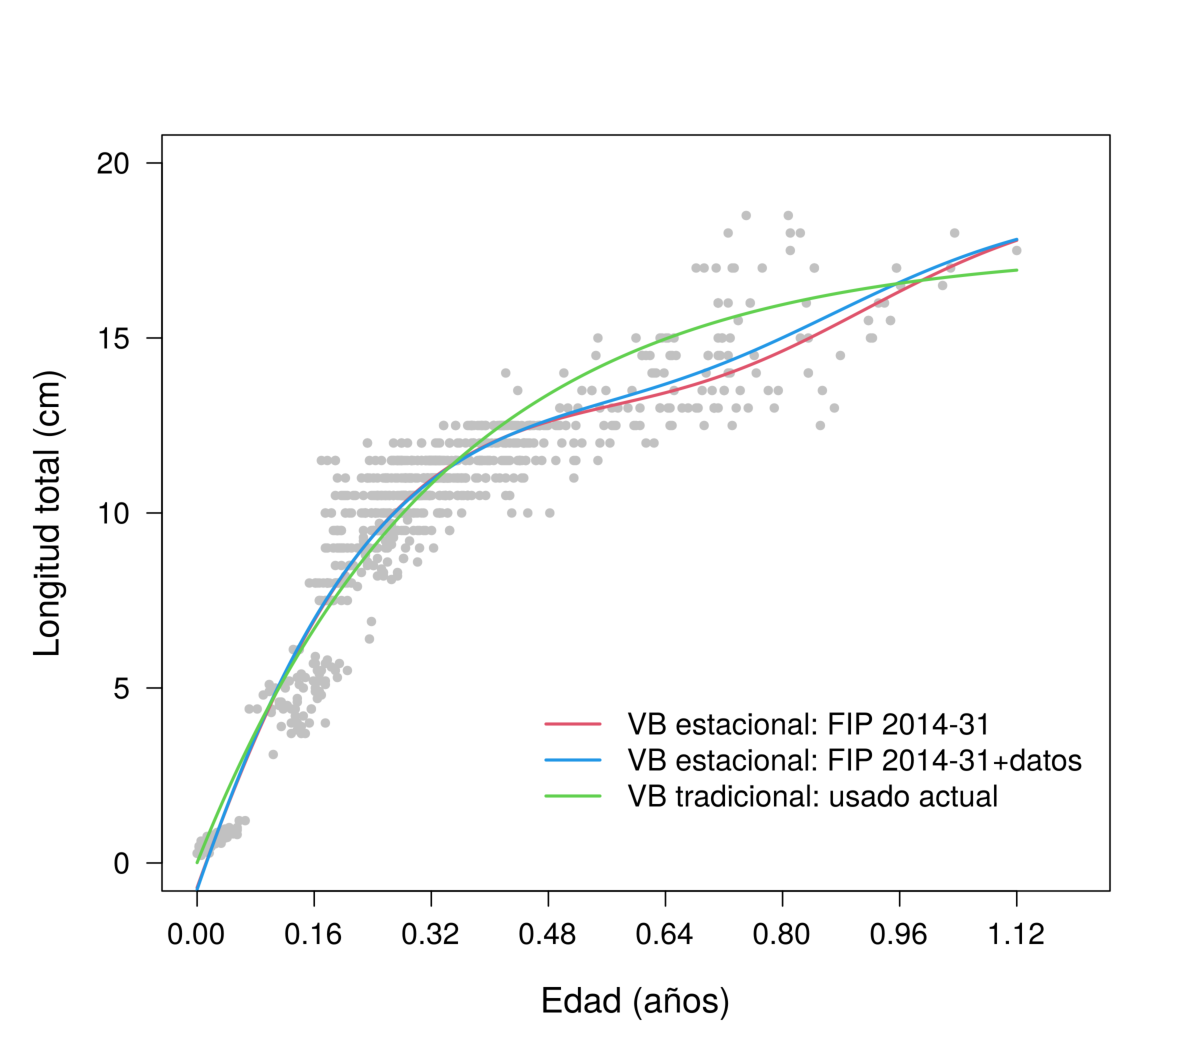
\includegraphics[width=11cm,height=9cm]{Figuras/figura17.pdf}
 \caption{Funci\'on de crecimiento de von Bertalanffy tradicional y estacional para la anchoveta del sur de Per\'u y norte de Chile.}
 \label{Fig17}
\end{figure}


\paragraph{f) Mortalidad natural}

\quad

La mortalidad natural fue calculada a trav\'es de diferentes modelos
bio-anal\'ogicos existentes en la literatura seg\'un los par\'ametros de
crecimiento anteriormente se\~{n}alados (\textbf{Tabla \ref{Tab10}}). Estos
modelos entregan un valor superior a dos (\textbf{Tabla \ref{Tab11}}),
para lo cual se utiliz\'o un valor de $M=1.1$ (semestre$^{-1}$) para
la tasa de mortalidad natural ($M$), valor usado como constante para
todas las edades y a\~{n}os.\\

\vspace{0.5cm}
\begin{table}[htb!]
 \caption{M\'etodos emp\'iricos para estimar la mortalidad natural.}
 \label{Tab11}
 \vspace{0.01cm}
 \centering
 \vspace{0.2cm}
 \small
 \begin{tabular}{lccc}
 \noalign{\vskip 0.1cm}
 \cline{2-4} & \multicolumn{3}{c}{Edad te\'orica m\'axima} \\
 \hline
 \noalign{\vskip 0.1cm}
  M\'etodo  & \--- & 1 & 2 \\
 \hline
 \noalign{\vskip 0.2cm}
 Rikhter y Efanov (1976) & 2.78 & \--- & \--- \\
 Pauly (1980) & 1.74 & \--- & \--- \\
 Taylor (1958, 1960) & \--- & 2.16 & 1.99 \\
 Hoening (1983) & \--- & 2.16 & 2.14 \\
 Alverson y Carney (1975) & \--- & 2.33 & 2.28 \\
 Alagaraja (1984) & \--- & 2.33 & 2.30 \\
 Hewitt y Hoening (2005) & \--- & 2.14 & 2.11 \\
 \noalign{\vskip 0.1cm}
 \hline
 \noalign{\vskip 0.1cm}
 \textbf{Promedio} & \textbf{2.26} & \textbf{2.22} & \textbf{2.17} \\
 \noalign{\vskip 0.1cm}
 \hline
 \noalign{\vskip 0.2cm}
 \multicolumn{1}{l}{(1) $T_{max}=t_{0}+\frac{3}{k}$}
 \end{tabular}
\end{table}


\paragraph{g) Indicadores de abundancia independientes de la pesquer\'ia}

\quad

Las estimaciones actualizadas de biomasa desovante al 2020 y disponible
para la evaluaci\'on de stock se entregan en la
\textbf{Tabla \ref{Tab12}}. Para prop\'ositos de la evaluaci\'on de stock,
el \'indice de biomasa desovante utilizado corresponde al reportado por
Claramunt \textit{et al}. (2014). En el 2014 la estimaci\'on de biomasa
desovante alcanz\'o un valor de 399 mil toneladas. En el 2015 la
estimaci\'in de biomasa desovante subi\'o levemente a las 436 mil toneladas,
luego en el 2016 fue de 461 mil toneladas y en el 2017 fue de 201 mil
toneladas, lo que representa una disminuci\'on del 56\% con respecto al
2016. En el 2018 la biomasa desovante estimada aumento a las 799 mil
toneladas y en el 2019 esta fue de 645 mil toneladas. Sin embargo, en el
2020 este valor alcanz\'o las 297 mil toneladas. En la
\textbf{Tabla \ref{Tab12}} se muestran los \'indices provenientes de las
evaluaciones hidroac\'usticas por a\~{n}o e incluye: i) la biomasa total de
Per\'u realizados durante los a\~{n}os 1990 al 2020 y la biomasa total para el
norte de Chile (Castillo \textit{et al}., 2009, 2010, 2011, 2012, 2013).
Los cruceros peruanos fueron realizados durante el primer y segundo
semestre de cada a\~{n}o en que se tiene dicha informaci\'on en Per\'u. Para el
norte de Chile se incluye tambi\'en la estructura de tama\~{n}os disponible
para la abundancia total estimada durante los a\~{n}os 2000-2002 y 2007-2020
y la fecha en que se desarroll\'o el crucero ac\'ustico. La actualizaci\'on de
los registros peruanos se efectu\'o a trav\'es de los Talleres IMARPE-IFOP
de Evaluaci\'on Conjunta del Stock de Anchoveta del Sur de Per\'u y Norte de
Chile, el \'ultimo realizado entre el 3 y 7 de diciembre del 2018 en el
Club Alem\'an, Valpara\'iso, Chile.

En enero 2015, el IMARPE report\'o en la zona sur del Per\'u una biomasa
total de 534 mil toneladas, de las cuales el 94\% estaba compuesto por
biomasa de reclutas (Oficio PRODUCE 100-556-2014), individuos menores a
11.5 cm. Asimismo, poco antes y en diciembre del 2014 IFOP hab\'ia
registrado una biomasa de 410 mil toneladas cuya incidencia de reclutas
alcanzaba el 60\% en peso. Y para el 2016 se estima una biomasa total de
307 mil toneladas para el norte de Chile y en el 2017 este valor fue de
105 mil toneladas. Sin embargo, este valor sube dr\'asticamente a 793 mil
toneladas de biomasa total en el 2018, lo que representa un aumento de
m\'as de seis veces de magnitud. Pero en el 2019 este valor cae
dr\'asticamente a las 230 mil toneladas. Y en el 2020, sube levemente a
las 264 mil toneladas. En la \textbf{Tabla \ref{Tab13}} muestra un resumen de la temporalidad de
las evaluaciones directas llevadas a cabo en el norte de Chile. Anterior
al a\~{n}o 2007 los cruceros se realizaban en distintos meses, ya que el
criterio era evaluar el m\'aximo reclutamiento basado en el m\'aximo desove
a fines de agosto (ver \textbf{Figura \ref{Fig2}}). Posterior al a\~{n}o
2008, se fij\'o la fecha para el crucero del norte de Chile. Las
estructuras de tallas de los cruceros ac\'usticos de anchoveta est\'an
disponibles desde el 2000 hasta 2002 y desde el 2007 hasta el 2020. Esta
informaci\'on es relevante dado por la presencia de individuos de menor
tama\~{n}o (individuos desde los 2.5 cm), dando cuenta de los reclutas que
est\'an ingresando a la pesquer\'ia, y por el extenso periodo que abarca
esta informaci\'on (\textbf{Figura \ref{Fig18}}).\\

La \textbf{Figura \ref{Fig19}} muestra los \'indices utilizados en la
actual evaluaci\'on de stock al segundo semestre del 2020. En el caso de
la biomasa total ac\'ustica del Per\'u, representa la fracci\'on
correspondiente a la regi\'on sur de Per\'u (16-18\degree 21`L.S.). En el
caso de la biomasa ac\'ustica de Chile representa la totalidad de la
biomasa estimada desde los 18\degree 21' hasta los 24\degree L.S. Las
estimaciones hechas a fines de primavera de los a\~{n}os 2014, 2015 y 2016
se han registrado altos valores, con un promedio de 334 ($\pm$) 66) mil
toneladas, un gran porcentaje de estas biomasas corresponde a la
fracci\'on juvenil del stock. Durante el 2017 este valor cae a 105 mil
toneladas para luego expandirse a 793 mil toneladas durante el 2018,
valor m\'as alto de la serie hist\'orica. Sin embargo, este valor cae a 230
mil toneladas en el 2019 y se recupera levemente en el 2020. Por otra
parte, la biomasa desovante estimada en el segundo semestre del 2017
alcanz\'o un valor de 201 mil toneladas, el valor m\'as bajo de toda la
serie hist\'orica estimada por el m\'etodo de producci\'on diaria de huevos
para la anchoveta del norte de Chile. Pero la estimaci\'on hecha en el
2018, la biomasa desovante alcanz\'o un valor de 799 mil toneladas,
mostrando un aumento de casi cuatro veces con respecto al valor
observado en el 2017 (\textbf{Figura \ref{Fig19}}). Sin embargo, este
valor cae levemente en el 2019 a 651 mil toneladas y m\'as a\'un en el 2020
a 297 mil toneladas, valor muy cerano al m\'inimo del 2017.


\vspace{0.5cm}
\begin{table}[htb!]
 \caption{Biomasa estimada a trav\'es del M\'etodo de Producci\'on de Huevos (MPH) y cruceros ac\'usticos del stock de anchoveta del sur de Per\'u y norte de Chile.}
 \label{Tab12}
 \centering
 \small
 \begin{tabular}{lrrr}
 \hline\noalign{\vskip 0.1cm}
 A\~{n}o & MPH & Ac\'ustica Per\'u & Ac\'ustica Chile \\
 \hline\noalign{\vskip 0.1cm}
  1990  &  \---   &  187.000  &  \---  \\
 1991  &  \---   &   558.000  &  \---  \\
 1992  &  314.232  &   482.000  &  \---  \\
 1993  &  \---   &   893.000  &  \---  \\
 1994  &  \---   &   744.000  &  \---  \\
 1995  &  465.696  &  2.667.000  &  \---  \\
 1996  &  253.356  &   648.000  &  385.881  \\
 1997  &  744.838  &   745.000  &  \---  \\  
 1998  &  \---   &  1.306.000  &  957.868  \\
 1999  &  973.292  &   178.000  &  \---  \\
 2000  &  608.087  &   522.000  &  959.791  \\
 2001  &  765.885  &   199.000  &  317.977  \\
 2002  & 1.503.911  &  1008.000  &  \---  \\
 2003  & 1.238.731  &   839.000  &  \---  \\
 2004  &  668.979  &   682.000  &  \---  \\
 2005  & 1.520.754  &  1.375.000  &  \---  \\
 2006  & 1.081.156  &   283.000  &  \---  \\
 2007  &  240.727  &  1.318.000  &  713.012  \\
 2008  &  532.132  &   554.000  &  135.550  \\
 2009  &  287.916  &   425.000  &  456.341  \\
 2010  &  \---   &  1.274.000  &  253.861  \\
 2011  &  795.056  &   613.000  &  170.405  \\
 2012  &  672.077  &  2.271.000  &  299.520  \\
 2013  &  520.336  &  2.013.000  &  163.002  \\
 2014  &  399.605  &   884.000  &  410.660  \\
 2015  &  436.014  &   534.000  &  285.644  \\
 2016  &  461.000  &   370.000  &  307.129  \\
 2017  &  201.178  &  1.487.000  &  105.841  \\
 2018  &  799.400  &  1.156.000  &  793.242  \\
 2019  &  645.891  &  2.968.000  &  230.206  \\
 2020  &  297.628  &  2.035.000 & 264.438 \\
 \hline
 \end{tabular}
\end{table}



\vspace{0.5cm}
\begin{table}[htb!]
 \caption{Periodo de realizaci\'on (semanas) de los cruceros hidroac\'usticos de anchoveta de la zona norte de Chile.}
 \label{Tab13}
 \centering
 \small
 \begin{tabular}{lccccccccccccccccc}
 & &\multicolumn{4}{c}{Noviembre} &\multicolumn{4}{c}{Diciembre} &\multicolumn{4}{c}{Enero} &\multicolumn{4}{c}{Febrero}\\
 \hline\noalign{\vskip 0.1cm}
 Crucero & A\~{n}o & 1 & 2 & 3 & 4 & 1 & 2 & 3 & 4 & 1 & 2 & 3 & 4 & 1 & 2 & 3 & 4 \\
 \hline\noalign{\vskip 0.1cm}
 RECLAN9601 & 1996 & & & & & & & & & \cellcolor{Gray}X & \cellcolor{Gray}X & \cellcolor{Gray}X & & & & & \\
 RECLAN9611 & 1997 & & & \cellcolor{Gray}X & \cellcolor{Gray}X & \cellcolor{Gray}X & & & & & & & & & & & \\
 RECLAN9801 & 1998 & & & & & & & & & & \cellcolor{Gray}X & \cellcolor{Gray}X & \cellcolor{Gray}X & & & & \\
 RECLAN9811 & 1999 & & & & \cellcolor{Gray}X & \cellcolor{Gray}X & \cellcolor{Gray}X & & & & & & & & & & \\
 RECLAN0001 & 2000 & & & & & & & & & & \cellcolor{Gray}X & \cellcolor{Gray}X & \cellcolor{Gray}X & & & & \\
 RECLAN0012 & 2001 & & & & & \cellcolor{Gray}X & \cellcolor{Gray}X & \cellcolor{Gray}X & & & & & & & & & \\
 RECLAN0111 & 2002 & & & & \cellcolor{Gray}X & \cellcolor{Gray}X & \cellcolor{Gray}X & & & & & & & & & & \\
 RECLAN0702 & 2007 & & & & & & & & & & & & & \cellcolor{Gray}X & \cellcolor{Gray}X & \cellcolor{Gray}X & \\
 RECLAN0712 & 2008 & & & & & & & & & & & & & & & & \\
 RECLAN0812 & 2009 & & & & & \cellcolor{Gray}X & \cellcolor{Gray}X & \cellcolor{Gray}X & & & & & & & & & \\
 RECLAN0912 & 2010 & & & & & \cellcolor{Gray}X & \cellcolor{Gray}X & \cellcolor{Gray}X & & & & & & & & & \\
 RECLAN1012 & 2011 & & & & \cellcolor{Gray}X & \cellcolor{Gray}X & \cellcolor{Gray}X & \cellcolor{Gray}X & & & & & & & & & \\
 RECLAN1112 & 2012 & & & & \cellcolor{Gray}X & \cellcolor{Gray}X & \cellcolor{Gray}X & \cellcolor{Gray}X & & & & & & & & & \\
 RECLAN1212 & 2013 & & & & \cellcolor{Gray}X & \cellcolor{Gray}X & \cellcolor{Gray}X & \cellcolor{Gray}X & & & & & & & & & \\
 RECLAN1312 & 2014 & & & & \cellcolor{Gray}X & \cellcolor{Gray}X & \cellcolor{Gray}X & \cellcolor{Gray}X & & & & & & & & & \\
 RECLAN & 2015 & & & & \cellcolor{Gray}X & \cellcolor{Gray}X & \cellcolor{Gray}X & \cellcolor{Gray}X & & & & & & & & & \\
 RECLAN & 2016 & & & & \cellcolor{Gray}X & \cellcolor{Gray}X & \cellcolor{Gray}X & \cellcolor{Gray}X & & & & & & & & & \\
 RECLAN & 2017 & & & & \cellcolor{Gray}X & \cellcolor{Gray}X & \cellcolor{Gray}X & \cellcolor{Gray}X & & & & & & & & & \\
 RECLAN & 2018 & & & & \cellcolor{Gray}X & \cellcolor{Gray}X & \cellcolor{Gray}X & \cellcolor{Gray}X & & & & & & & & & \\
 RECLAN & 2019 & & & & \cellcolor{Gray}X & \cellcolor{Gray}X & \cellcolor{Gray}X & \cellcolor{Gray}X & & & & & & & & & \\
 RECLAN & 2020 & & & & \cellcolor{Gray}X & \cellcolor{Gray}X & \cellcolor{Gray}X & \cellcolor{Gray}X & & & & & & & & & \\
 \hline
 \end{tabular}
\end{table}

\vspace{0.5cm}
\begin{figure}[htb!]
 \centering
 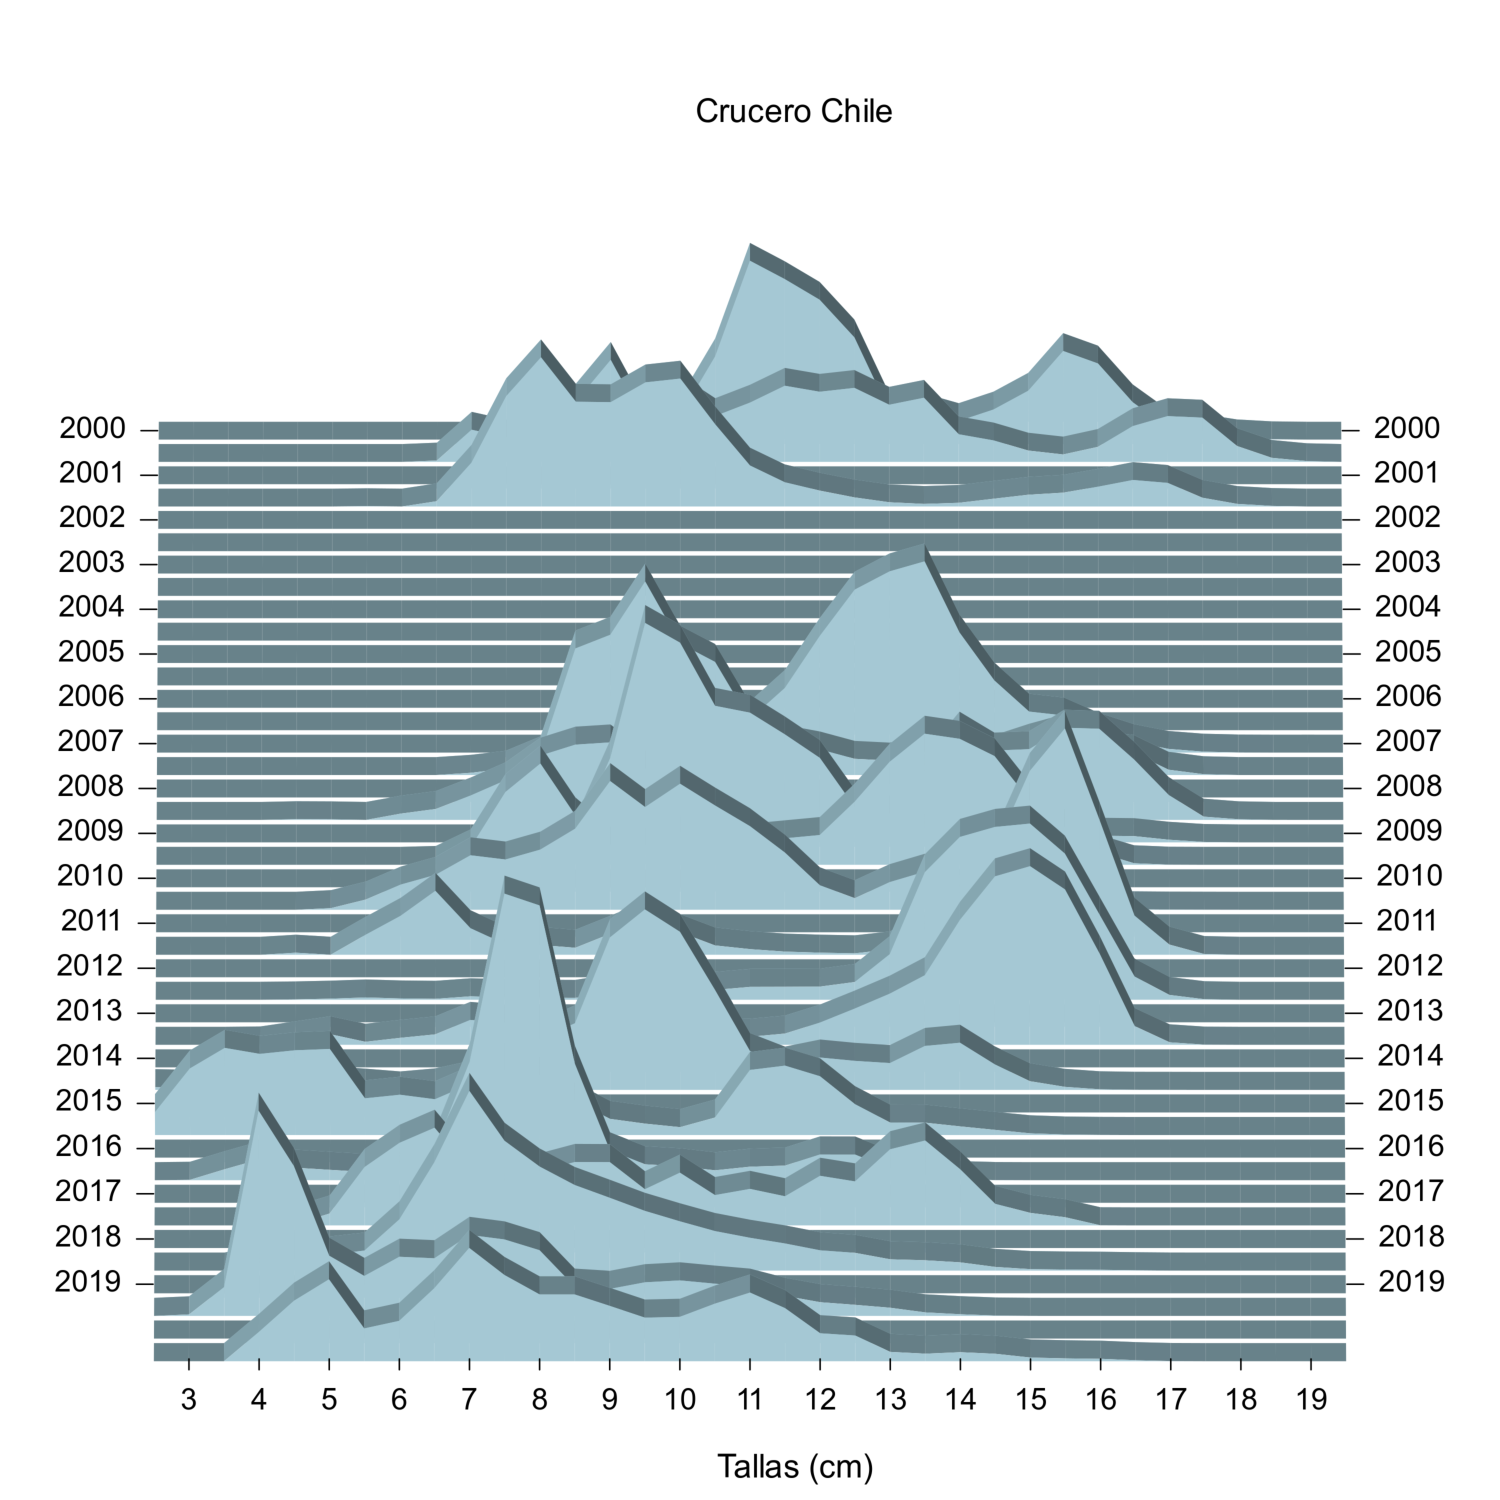
\includegraphics[width=10cm,height=9cm]{Figuras/figura18.pdf}
 \caption{Proporci\'on por tallas de la abundancia del crucero ac\'ustico en el norte de Chile (2000-2001 y 2007- 2020).}
 \label{Fig18}
\end{figure}




\vspace{0.5cm}
\begin{figure}[htb!]
 \centering
 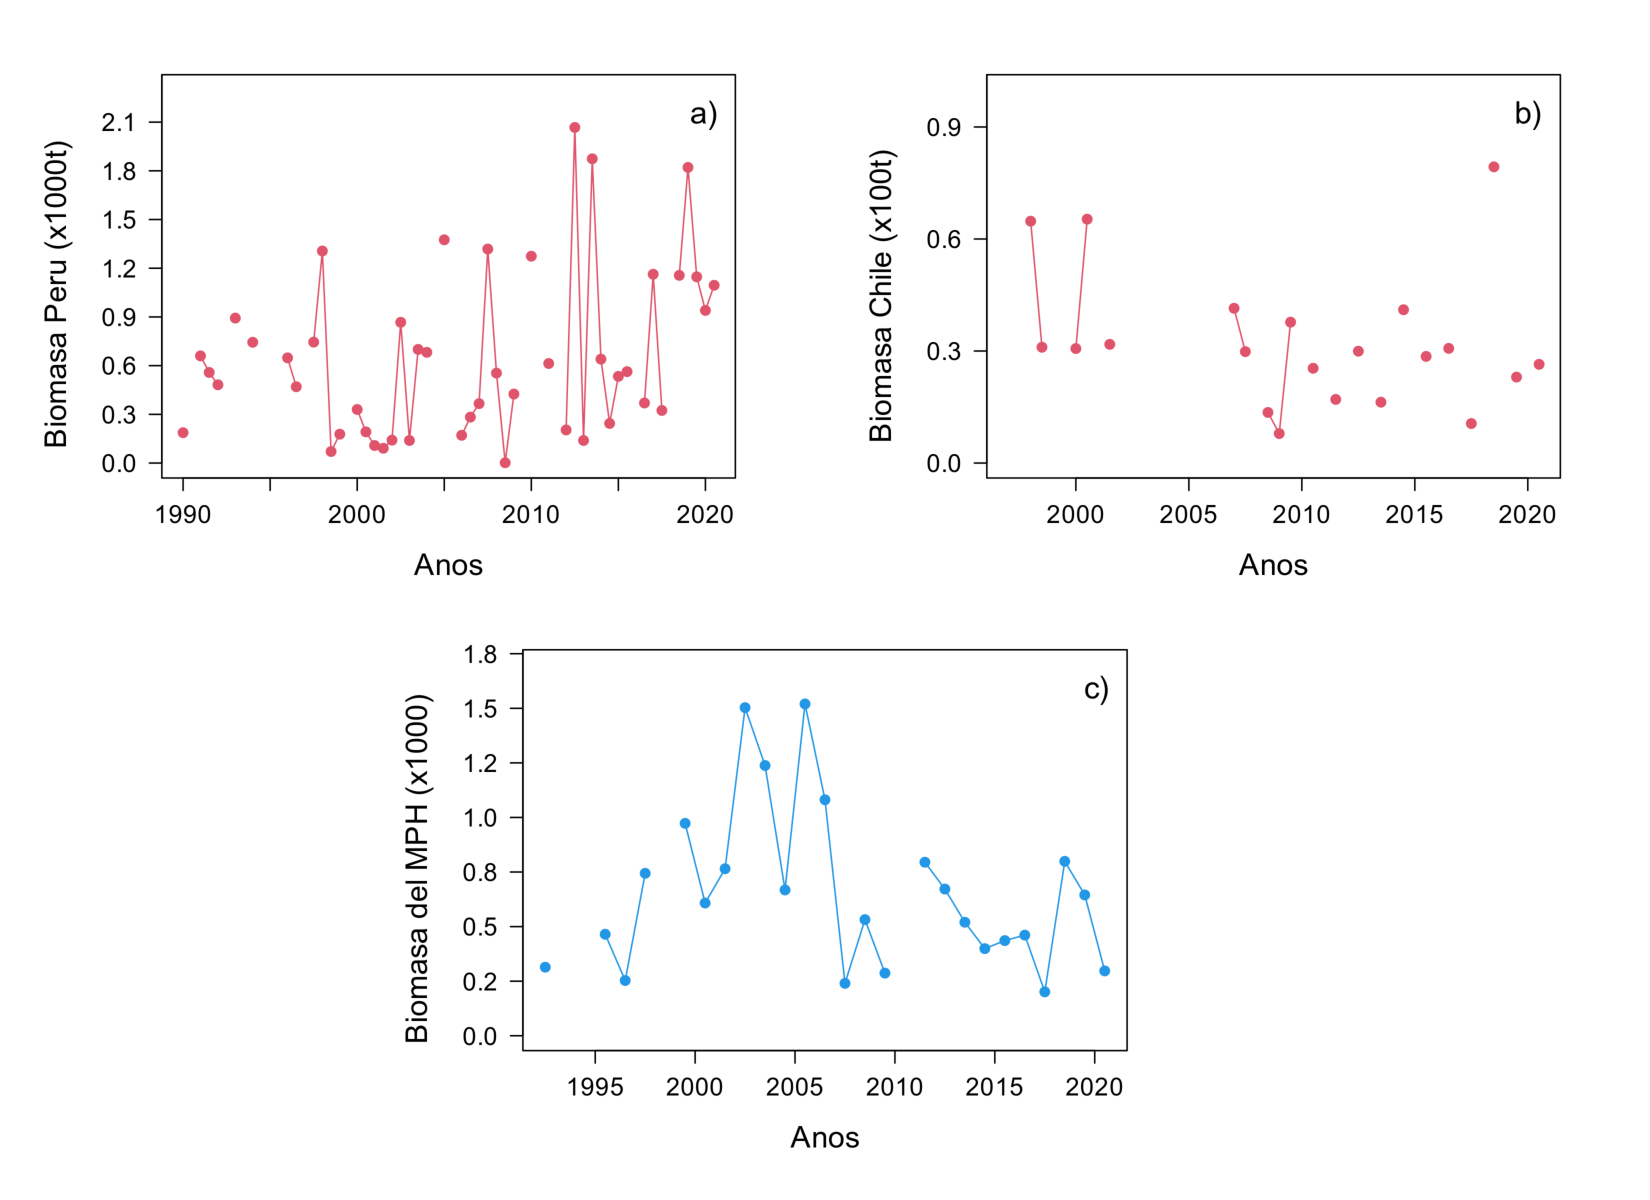
\includegraphics[width=12cm,height=11cm]{Figuras/figura19.pdf}
 \caption{\'Indices considerados en la evaluaci\'on del stock de anchoveta del sur de Per\'u y norte de Chile al segundo semestre del 2020, en a) la biomasa total ac\'ustica del Per\'u, b) la biomasa total ac\'ustica de Chile y c) biomasa desovante estimada a partir del MPH del norte de Chile.}
 \label{Fig19}
\end{figure}


\clearpage
\newpage

\subsection{Objetivo espec\'ifico 4.}

\textit{\textquotedblleft Informar el avance del Programa de Mejoramiento Continuo de la Calidad en la Asesor\'ia Cient\'ifica (PMCCAC) realizado durante el presente estudio, respecto al cumplimiento de recomendaciones formuladas en procesos de RPEI y priorizadas por el CCT, cuando corresponda.\textquotedblright}
\vspace{-0.2cm}


\subsubsection{Mejoras realizadas al modelo de evaluaci\'on de stock}

La principal mejora realizada al modelo de evaluaci\'on de stock para la
anchoveta del sur de Per\'u y norte de Chile fue realizada en el taller de
revisi\'on por pares entre los d\'ias 11 al 13 de marzo del 2019 por el
Dr. James Ianelli, experto del centro de ciencia pesquera de Alaska de
la NOAA (National Oceanic and Atmospheric Administration). El taller dio
cuenta de la revisi\'on de los datos usados en la evaluaci\'on de stock, el
crecimiento de la anchoveta basado en micro incrementos diarios y el
supuesto de mortalidad natural usado, las hip\'otesis estructurales que
definen el modelo conceptual de la pesquer\'ia de la anchoveta del sur de
Per\'u y norte de Chile. Adem\'as, se revis\'o la din\'amica poblacional, los
modelos de los procesos y error, la configuraci\'on del modelo de
evaluaci\'on. Y finalmente, se revisaron los ajustes del modelo de
evaluaci\'on a los datos usados, las variables poblacionales estimadas por
el modelo, el desempe\~{n}o del modelo, an\'alisis retrospectivo, puntos
biol\'ogicos de referencia y estatus del recurso estudiado. Finalmente,
durante los d\'ias 8 al 12 de julio del 2019 se realiz\'o el Taller
\textquotedblleft Benchmark Stock Assessment\textquotedblright 
para la anchoveta del sur de Per\'u y norte de Chile
por la Dra. Carolina Minte-Vera, experta de la Comisi\'on
Inter-Americana del At\'un Tropical (IATTC) con sede en la Jolla,
California, USA. Este taller tuvo la finalidad de incorporar las
sugerencias del Dr. Ianelli para mejorar el modelo de evaluaci\'on de
stock antes de que el modelo pueda ser usado con fines para el manejo
pesquero.

Posterior a este taller, se ha continuado haciendo mejoras al modelo de
evaluaci\'on, primero, la incorporaci\'on de una selectividad tipo
doble-normal, con la capacidad de convertirse en log\'istica en caso que
los datos en las estructuras de tallas lo indiquen, dado el valor de la
varianza asignado al lado izquierdo de esta ecuaci\'on asignado por el
modelo. Esta mejora permite lidiar con las altas mortalidades por pesca
que se observan en el modelo log\'istico (las que alcanzan el l\'imite
superior establecido por el modelo) y que repercuten en el an\'alisis
retrospectivo cuando se registran las altas abundancias totales
estimadas a trav\'es del m\'etodo ac\'ustico y las bajas capturas que se
registra durante el a\~{n}o 2016. Segundo, otra mejora realizada que no
tiene relaci\'on con el c\'odigo del modelo de evaluaci\'on pero s\'i con el
tratamiento de la informaci\'on utilizada en el modelo de evaluaci\'on, es
la incorporaci\'on de la relaci\'on longitud-peso variable por semestre
desde el a\~{n}o 2001 hasta el 2020 (\textbf{Figura \ref{Fig15}}), debido
principalmente a la variabilidad que se han observado en las estructuras
de tallas de las capturas durante los \'ultimos veinte a\~{n}os
(\textbf{Figura \ref{Fig13}} y \textbf{Figura \ref{Fig14}}), y m\'as a\'un
durante los \'ultimos cinco a\~{n}os, en que la talla media registra valores
por debajo de los 12 cm de longitud total, lo cual implica un menor peso
en los individuos capturados.


\subsubsection{Avances en la reducci\'on de brechas}

El gran desaf\'io que presentan los peque\~{n}os peces pel\'agicos a nivel
mundial, y m\'as a\'un en la anchoveta de la zona norte de Chile dado su
r\'apido crecimiento y alta mortalidad natural, es intentar predecir los
reclutamientos futuros durante la proyecci\'on del stock. Actualmente, la
elecci\'on de los reclutamientos futuros para cada semestre, se
seleccionan seg\'un la historia de los reclutamientos promedios ocurridos
durante el primer y segundo semestre por separado
(\textbf{Figura \ref{Fig9}}). La principal caracter\'istica de esta
metodolog\'ia es que los reclutamientos futuros son tratados como eventos
independentes. Sin embargo, el modelo de evaluaci\'on presenta una
tendencia a sobre-estimar los reclutamientos del primer hito de asesor\'ia
cuando se incorporan nuevos datos en el segundo hito de asesor\'ia
(\textbf{Figura \ref{Fig20}}). Esto debido principalmente a la reducci\'on
de las capturas durante los \'ultimos semestres y que podr\'ia tener alguna
relaci\'on con las tendencias que presenta la serie de captura en el
mediano plazo, 3-4 a\~{n}os (\textbf{Figura \ref{Fig11}}). Este patr\'on
retrospectivo en los reclutamientos hace necesario plantearse algunos
escenarios sobre los supuestos en los reclutamientos que ser\'an
ingresados durante la proyecci\'on del stock de anchoveta, tanto para el
primer hito de asesor\'ia (septiembre), como en el segundo hito (marzo) de
asesora\'ia.

\pagebreak

\vspace{0.5cm}
\begin{figure}[htb!]
 \centering
 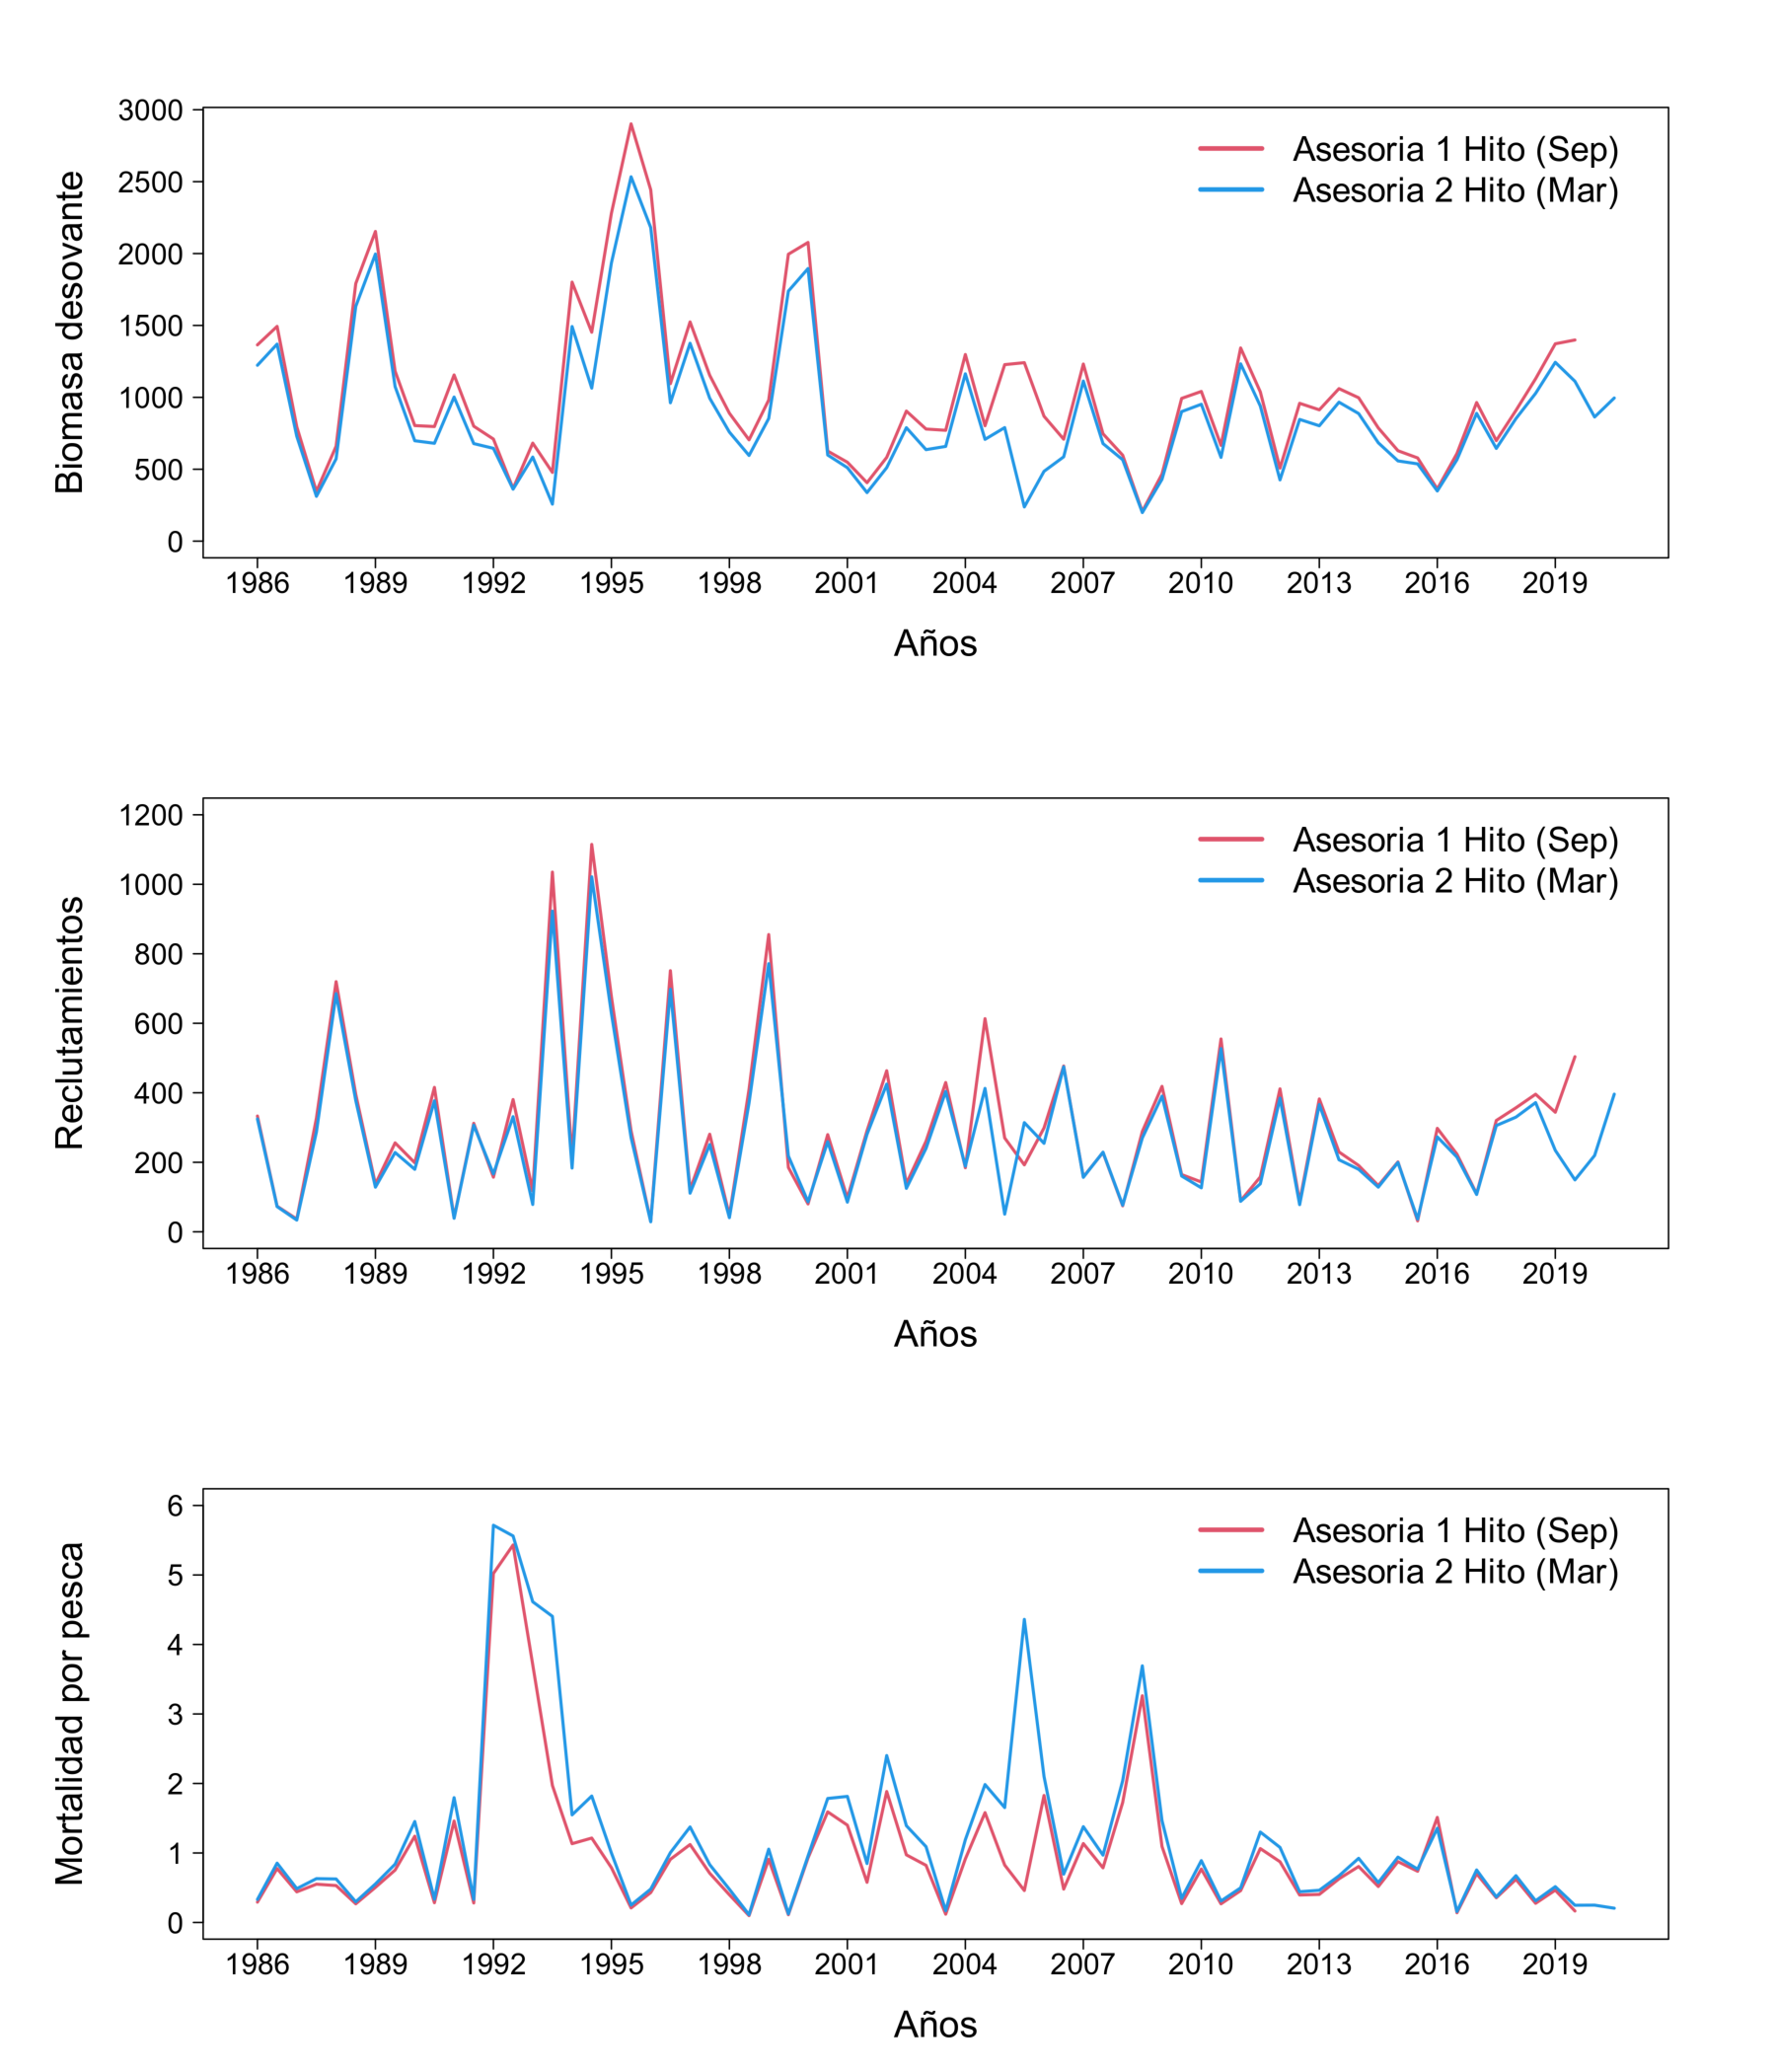
\includegraphics[width=15cm,height=12cm]{Figuras/figura20.pdf}
 \caption{Estimaciones de las principales variables de estado durante el ciclo de asesor\'ia anual. El Hito 1 corresponde a la asesor\'ia de septiembre 2020 y el Hito 2 a la asesor\'ia del marzo del 2021.}
 \label{Fig20}
\end{figure}


\subsubsection{Revisi\'on del roceso de estimaci\'on de CBA de anchoveta norte}

\quad

El proceso de estimaci\'on de la CBA anual para el stock de la anchoveta
del sur de Per\'u y norte de Chile tiene dos hitos: i) el primer hito de
asesor\'ia que ocurre en octubre de cada a\~{n}o, y es necesario proyectar el
stock de anchoveta cuatro semestres para estimar la CBA anual (3 y 4
semestre) y en el 1 y 2 semestre hay mortalidad por pesca conocida. 
Y ii) el segundo hito de asesor\'ia que ocurre en marzo de cada
a\~{n}o, y es necesario proyectar el stock de anchoveta dos semestres para
estimar la CBA anual (1 y 2 semestre). En cada uno de estos hitos es
necesario hacer supuestos sobre los niveles de reclutamientos (n\'umero de
individuos) que ser\'an ingresados en cada uno de los semestres
proyectados (4 y 2 semestres). Estos niveles de reclutamientos podr\'aan
corresponder a un promedio de ciertos reclutamientos que ocurrieron en
un periodo determinado (longitud de la serie), diferenciado por
semestres o un patr\'on inherente que ocurre dentro del a\~{n}o (sem1 $>$
sem2 o sem1 $<$ sem2) en un largo periodo de tiempo. O podr\'iamos hacer
alg\'un tipo de penalizaci\'on del \'ultimo reclutamiento estimado por el
modelo dado el patr\'on retrospectivo que se observa en los reclutamientos
(\textbf{Figura \ref{Fig20}}). Para el caso de penalizar el reclutamiento,
se considera el l\'imite inferior del intervalo de confianza estimado
por el modelo para el \'ultimo reclutamiento. Para cada uno de los
hitos de asesor\'ia, se asumen que los reclutamientos ingresados
en cada uno de los semestres proyectados es considerado como un evento
independiente de un semestre a otro.

El resultados mostrados a continuaci\'on corresponde a modo de ejemplo,
donde el modelo de evaluaci\'on entrega estimaciones de todos los grupos
etarios hasta el 2019.5, se considera la mortalidad por pesca total
(flota chilena + flota peruana) y los pesos medios del \'ultimo semestre.
La mortalidad por pesca total es ponderada por la mortalidad por pesca
que produce el RMS, equivalente al 55\%BDPR.


\subsubsection{Primer hito}

\quad

Para el primer hito de asesor\'ia se evaluaron los siguientes escenarios
\textbf{Tabla \ref{Tab14}}. Los resultados de las proyecciones muestran
que la biomasa desovante deber\'ia fluctuar entre un mill\'on 776 mil
toneladas y 927 mil toneladas para el escenario E1, valores muy
similares para el escenario E2. Para el escenario E3, la biomasa
desovante deber\'ia fluctuar entre un mill\'on 225 mil toneladas y 813 mil
toneladas, valores muy similares para el escenario E4
(\textbf{Figura \ref{Fig21}}). Para todos los escenarios evaluados
durante el primer y segundo semestre proyectado, la captura tienen
valores muy similares, debido a que esta es conocida
(\textbf{Figura \ref{Fig21}} y \textbf{Tabla \ref{Tab15}}). Para el
tercer semestre proyectado la captura registra un valor m\'aximo de 432
mil toneladas para el escenario E1 y un valor m\'inimo de 399 mil
toneladas para el escenario E4. Y para el cuatro semestre proyectado la
captura registra un valor m\'aximo de 343 mil toneladas para el escenario
E1 y un valor m\'inimo de 326 mil toneladas para el escenario E4. En
t\'erminos de la reducci\'on de la biomasa desovante de largo plazo del
stock de anchoveta, todos los escenarios evaluados convergen al final de
la proyecci\'on a un valor por sobre el objetivo de manejo pesquero,
indicando que el stock de anchoveta es altamente productivo dado los
niveles de reclutamientos ingresados durante la proyecci\'on
(\textbf{Figura \ref{Fig21}}).\\

\vspace{0.5cm}
\begin{table}[htb!]
 \caption{Escenarios de proyecci\'on usados en el primer hito de asesor\'ia.}
 \label{Tab14}
 \centering
 \small
 \begin{tabular}{ll}
 \hline\noalign{\vskip 0.1cm}
 Escenario & Descripci\'on \\
 \hline\noalign{\vskip 0.1cm}
 E1  &  Reclutamientos promedios desde el 2000 hasta el 2019.5 (Caso base)  \\
 E2  &  Reclutamientos promedios desde el 2000 hasta el 2018.5  \\
 E3  &  E1 + penalizaci\'on \'ultimo reclutamiento (2019.5)  \\
 E4  &  E2 + penalizaci\'on \'ultimo reclutamiento (2019.5)  \\
 \hline
 \end{tabular}
\end{table}

\vspace{0.5cm}
\begin{figure}[htb!]
 \centering
 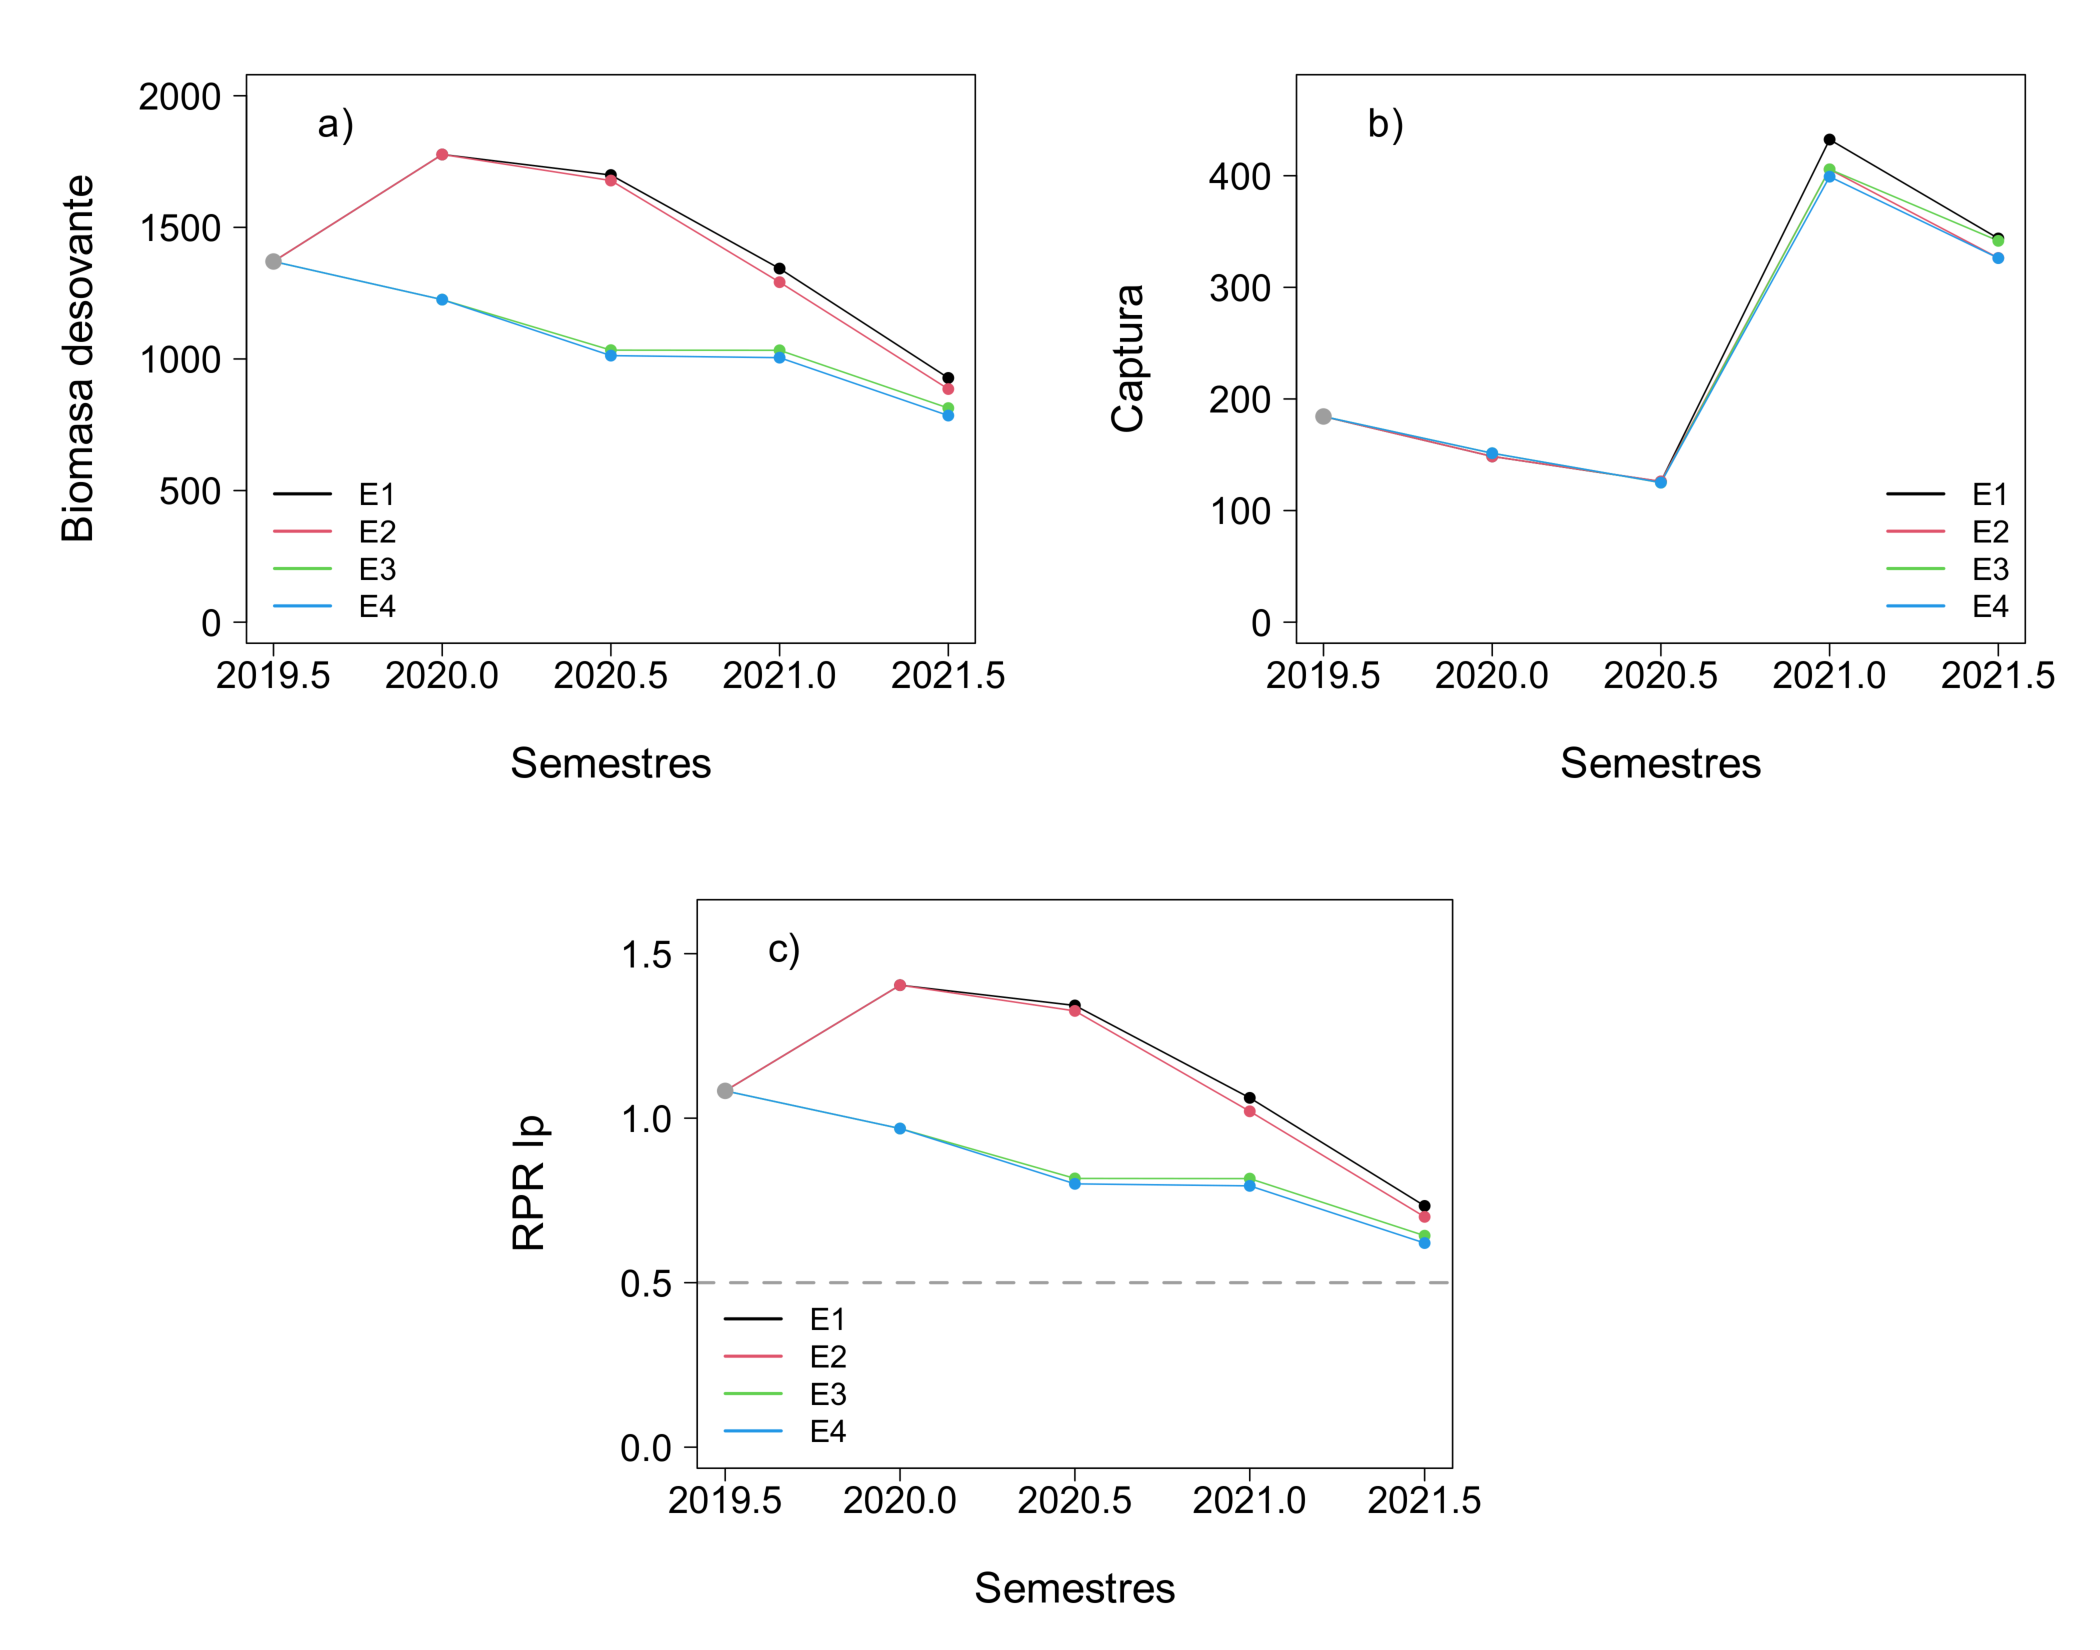
\includegraphics[width=13cm,height=11cm]{Figuras/figura21.pdf}
 \caption{Biomasa desovante (a), captura (b) y RPR largo plazao (c) proyectado para el primer hito de asesor\'ia.}
 \label{Fig21}
\end{figure}

\vspace{0.5cm}
\begin{table}[htb!]
 \caption{CBA semestral proyectada (2020-2021) y anual para el 2021 para el stock de anchoveta dado el criterio del F=F$_{RMS}$ y los diferentes escenarios evaluados.}
 \label{Tab15}
 \centering
 \small
 \begin{tabular}{lccccc}
 \hline\noalign{\vskip 0.1cm}
 Escenario & 2020.0 & 2020.5 & 2021.0 & 2021.5 & 2021$_{TOT}$ \\
 \hline\noalign{\vskip 0.1cm}
 E1  & 148.5 & 125.9 & 432.4 & 343.8 & 776.2  \\
 E2  & 148.5 & 126.1 & 405.6 & 326.3 & 731.9 \\
 E3  & 151.4 & 124.9 & 405.6 & 341.6 & 747.2 \\
 E4  & 151.4 & 125.0 & 399.1 & 326.1 & 725.2  \\
 \hline
 \end{tabular}
\end{table}

\pagebreak


\subsubsection{Aporte de cada grupo de edad a la captura proyectada por semestre}

\quad

Durante la proyecci\'on del stock de anchoveta se estim\'o la captura en
n\'umero de individuos por grupo de edad (Baranov, 1918), y luego fue
dividida por la suma total de todos los grupos de edad. Este porcentaje
por grupo de edad en la captura es presentado en las
\textbf{Tabla \ref{Tab16}}, \textbf{Tabla \ref{Tab17}},
\textbf{Tabla \ref{Tab18}} y \textbf{Tabla \ref{Tab19}} para el
escenario E1, E2, E3 y E4, respectivamente. Independiente del escenario
evaluado, el grupo de edad 1 (6 meses) es que mayor porcentaje aporta a
la captura semestral. Para el escenario E1 y E2 este valor var\'ia entre
un 78\% y un 91\%, y para el escenario E3 y E4 este valor varia entre un
78\% y un 83\%. En general, los grupos de edades 0 (reclutas), 1 (6
meses) y 2 (1 a\~{n}o) aportan el 100\% de la captural semestral para los
diferentes escenarios evaluados.\\

\vspace{0.5cm}
\begin{table}[htb!]
 \caption{Porcentaje por grupo de edad en la captura proyectada (2020-2021) para el escenario E1.}
 \label{Tab16}
 \centering
 \small
 \begin{tabular}{lcccc}
 \hline\noalign{\vskip 0.1cm}
 Edad & 2020.0 & 2020.5 & 2021.0 & 2021.5 \\
 \hline\noalign{\vskip 0.1cm}
 0 & 0.041 & 0.090 & 0.088 & 0.123  \\
 \rowcolor{Gray}
 1 & 0.914 & 0.787 & 0.848 & 0.831 \\
 2 & 0.043 & 0.120 & 0.059 & 0.042 \\
 3 & 0.001 & 0.002 & 0.003 & 0.001  \\
 \hline
 \rowcolor{Gray}
 Suma(0:2) & 0.999 & 0.998 & 0.996 & 0.998 \\
 \hline
 \end{tabular}
\end{table}


\vspace{0.5cm}
\begin{table}[htb!]
 \caption{Porcentaje por grupo de edad en la captura proyectada (2020-2021) para el escenario E2.}
 \label{Tab17}
 \centering
 \small
 \begin{tabular}{lcccc}
 \hline\noalign{\vskip 0.1cm}
 Edad & 2020.0 & 2020.5 & 2021.0 & 2021.5 \\
 \hline\noalign{\vskip 0.1cm}
 0 & 0.039 & 0.088 & 0.089 & 0.122  \\
 \rowcolor{Gray}
 1 & 0.916 & 0.783 & 0.846 & 0.833 \\
 2 & 0.043 & 0.126 & 0.060 & 0.042 \\
 3 & 0.001 & 0.002 & 0.003 & 0.001  \\
 \hline
 \rowcolor{Gray}
 Suma(0:2) & 0.999 & 0.997 & 0.996 & 0.998 \\
 \hline
 \end{tabular}
\end{table}


\vspace{0.5cm}
\begin{table}[htb!]
 \caption{Porcentaje por grupo de edad en la captura proyectada (2020-2021) para el escenario E3.}
 \label{Tab18}
 \centering
 \small
 \begin{tabular}{lcccc}
 \hline\noalign{\vskip 0.1cm}
 Edad & 2020.0 & 2020.5 & 2021.0 & 2021.5 \\
 \hline\noalign{\vskip 0.1cm}
 0 & 0.103 & 0.095 & 0.093 & 0.118  \\
 \rowcolor{Gray}
 1 & 0.788 & 0.861 & 0.845 & 0.839 \\
 2 & 0.105 & 0.041 & 0.059 & 0.040 \\
 3 & 0.002 & 0.002 & 0.001 & 0.001  \\
 \hline
 \rowcolor{Gray}
 Suma(0:2) & 0.997 & 0.997 & 0.998 & 0.998 \\
 \hline
 \end{tabular}
\end{table}


\vspace{0.5cm}
\begin{table}[htb!]
 \caption{Porcentaje por grupo de edad en la captura proyectada (2020-2021) para el escenario E4.}
 \label{Tab19}
 \centering
 \small
 \begin{tabular}{lcccc}
 \hline\noalign{\vskip 0.1cm}
 Edad & 2020.0 & 2020.5 & 2021.0 & 2021.5 \\
 \hline\noalign{\vskip 0.1cm}
 0 & 0.099 & 0.099 & 0.090 & 0.122  \\
 \rowcolor{Gray}
 1 & 0.792 & 0.855 & 0.851 & 0.833 \\
 2 & 0.106 & 0.043 & 0.056 & 0.042 \\
 3 & 0.002 & 0.002 & 0.001 & 0.001  \\
 \hline
 \rowcolor{Gray}
 Suma(0:2) & 0.997 & 0.997 & 0.998 & 0.998 \\
 \hline
 \end{tabular}
\end{table}

\pagebreak


\subsubsection{Abundancia semestral proyectada}

\quad

En las \textbf{Tabla \ref{Tab20}}, \textbf{Tabla \ref{Tab21}},
\textbf{Tabla \ref{Tab22}} y \textbf{Tabla \ref{Tab23}} se presentan las
matrices de abundancia en n\'umero durante la proyecci\'on del stock de
anchoveta. En estas se observan los diferentes supuestos
(\textbf{Tabla \ref{Tab14}}) aplicados para cada uno de los casos
evaluados. Adem\'as, se muestra la abundancia por grupo de edad al \'ultimo
semestre estimado por el modelo de evaluaci\'on, de manera de identificar
el \'ultimo reclutamiento estimado y el penalizado
(\textbf{Tabla \ref{Tab20}} y \textbf{Tabla \ref{Tab21}}). Y en las
\textbf{Tabla \ref{Tab22}} y \textbf{Tabla \ref{Tab23}} se muestra el
reclutamiento penalizado para el semestre 2019.5.\\


\vspace{0.5cm}
\begin{table}[htb!]
 \caption{Abundancia semestral proyectada (2019.5 - 2021.5) para el escenario E1.}
 \label{Tab20}
 \centering
 \small
 \begin{tabular}{lrrrrr}
 \hline\noalign{\vskip 0.1cm}
 Edad & 2019.5 & 2020.0 & 2020.5 & 2021.0 & 2021.5 \\
 \hline\noalign{\vskip 0.1cm}
 0 & \cellcolor{Gray1}498.17 & \cellcolor{Gray2}239.04 & \cellcolor{Gray3}283.16 & \cellcolor{Gray4}239.04 & 283.16  \\
 1 & 111.22 & \cellcolor{Gray1}165.00 & \cellcolor{Gray2}79.25 & \cellcolor{Gray3}93.69 & \cellcolor{Gray4}77.55 \\
 2 & 26.66 & 31.30 & \cellcolor{Gray1}47.98 & \cellcolor{Gray2}21.58 & \cellcolor{Gray3}13.19 \\
 3 & 8.57 & 8.52 & 10.09 & \cellcolor{Gray1}15.2 & \cellcolor{Gray2}5.85  \\
 4 & 1.89 & 2.84 & 2.83 & 3.34 & \cellcolor{Gray1}4.98 \\
 5 & 0.48 & 0.79 & 1.21 & 1.34 & 1.56 \\
 \hline
 \end{tabular}
\end{table}


\vspace{0.5cm}
\begin{table}[htb!]
 \caption{Abundancia semestral proyectada (2019.5 - 2021.5) para el escenario E2.}
 \label{Tab21}
 \centering
 \small
 \begin{tabular}{lrrrrr}
 \hline\noalign{\vskip 0.1cm}
 Edad & 2019.5 & 2020.0 & 2020.5 & 2021.0 & 2021.5 \\
 \hline\noalign{\vskip 0.1cm}
 0 & \cellcolor{Gray1}498.17 & \cellcolor{Gray2}227.26 & \cellcolor{Gray3}265.29 & \cellcolor{Gray4}227.26 & 265.29  \\
 1 & 111.22 & \cellcolor{Gray1}165.00 & \cellcolor{Gray2}75.34 & \cellcolor{Gray3}87.76 & \cellcolor{Gray4}73.73 \\
 2 & 26.66 & 31.30 & \cellcolor{Gray1}47.98 & \cellcolor{Gray2}20.34 & \cellcolor{Gray3}12.36 \\
 3 & 8.57 & 8.52 & 10.09 & \cellcolor{Gray1}15.19 & \cellcolor{Gray2}5.51  \\
 4 & 1.89 & 2.84 & 2.83 & 3.34 & \cellcolor{Gray1}4.97 \\
 5 & 0.48 & 0.79 & 1.21 & 1.34 & 1.56 \\
 \hline
 \end{tabular}
\end{table}


\vspace{0.5cm}
\begin{table}[htb!]
 \caption{Abundancia semestral proyectada (2019.5 - 2021.5) para el escenario E3.}
 \label{Tab22}
 \centering
 \small
 \begin{tabular}{lrrrrr}
 \hline\noalign{\vskip 0.1cm}
 Edad & 2019.5 & 2020.0 & 2020.5 & 2021.0 & 2021.5 \\
 \hline\noalign{\vskip 0.1cm}
 0 & \cellcolor{Gray1}185.15 & \cellcolor{Gray2}239.04 & \cellcolor{Gray3}267.53 & \cellcolor{Gray4}239.04 & 267.53  \\
 1 & 111.22 & \cellcolor{Gray1}61.44 & \cellcolor{Gray2}78.77 & \cellcolor{Gray3}88.40 & \cellcolor{Gray4}77.55 \\
 2 & 26.66 & 31.30 & \cellcolor{Gray1}14.57 & \cellcolor{Gray2}20.47 & \cellcolor{Gray3}12.45 \\
 3 & 8.57 & 8.52 & 9.61 & \cellcolor{Gray1}4.57 & \cellcolor{Gray2}5.55  \\
 4 & 1.89 & 2.84 & 2.82 & 3.18 & \cellcolor{Gray1}1.49 \\
 5 & 0.48 & 0.79 & 1.21 & 1.34 & 1.50 \\
 \hline
 \end{tabular}
\end{table}


\vspace{0.5cm}
\begin{table}[htb!]
 \caption{Abundancia semestral proyectada (2019.5 - 2021.5) para el escenario E4.}
 \label{Tab23}
 \centering
 \small
 \begin{tabular}{lrrrrr}
 \hline\noalign{\vskip 0.1cm}
 Edad & 2019.5 & 2020.0 & 2020.5 & 2021.0 & 2021.5 \\
 \hline\noalign{\vskip 0.1cm}
 0 & \cellcolor{Gray1}185.15 & \cellcolor{Gray2}227.26 & \cellcolor{Gray3}265.29 & \cellcolor{Gray4}227.26 & 265.29  \\
 1 & 111.22 & \cellcolor{Gray1}61.44 & \cellcolor{Gray2}74.88 & \cellcolor{Gray3}87.62 & \cellcolor{Gray4}73.73 \\
 2 & 26.66 & 31.30 & \cellcolor{Gray1}14.57 & \cellcolor{Gray2}19.21 & \cellcolor{Gray3}12.34 \\
 3 & 8.57 & 8.52 & 9.61 & \cellcolor{Gray1}4.56 & \cellcolor{Gray2}5.21  \\
 4 & 1.89 & 2.84 & 2.82 & 3.18 & \cellcolor{Gray1}1.49 \\
 5 & 0.48 & 0.79 & 1.21 & 1.34 & 1.50 \\
 \hline
 \end{tabular}
\end{table}

\pagebreak


\subsubsection{Segundo hito}

\quad

Para el segundo hito de asesoria se evaluaron los mismos escenarios del
primer hito \textbf{Tabla \ref{Tab14}}. Los resultados de las
proyecciones muestran que la biomasa desovante deber\'ia fluctuar entre un
mill\'on 665 mil toneladas y un mill\'on 116 mil toneladas para el escenario
E1, valores muy similares para el escenario E2. Para el escenario E3, la
biomasa desovante deber\'ia fluctuar entre un mill\'on 185 mil toneladas y
839 mil toneladas, valores muy similares para el escenario E4
(\textbf{Figura \ref{Fig22}}). Para el escenario E1 la captura fluctua
entre 737 mil toneladas y 371 mil toneladas, para el primer y segundo
semestre del 2020, respectivamente. Estos valores son muy similares para
el primer semestre del escenario E2 y se observa una diferencia cercana
a 20 toneladas en el segundo semestre. Y para el escenario E3 la captura
fluctua entre 329 mil toneladas y 332 mil toneladas para el primer y
segundo semestre del 2020, respectivamente. Estos valores son muy
similares para el primer semestre del escenario E4 y se observa una
diferencia cercana a 20 toneladas en el segundo semestre
(\textbf{Tabla \ref{Tab24}}). En t\'erminos de la reducci\'on dela biomasa
desovante de largo plazo del stock de anchoveta, todos los escenarios
evaluados muestran al final de la proyecci\'on un valor por sobre el
objetivo de manejo pesquero, indicando que el stock de anchoveta es
altamente productivo dado los niveles de reclutamientos ingresados
durante la proyecci\'on (\textbf{Figura \ref{Fig22}}).\\

\vspace{0.5cm}
\begin{figure}[htb!]
 \centering
 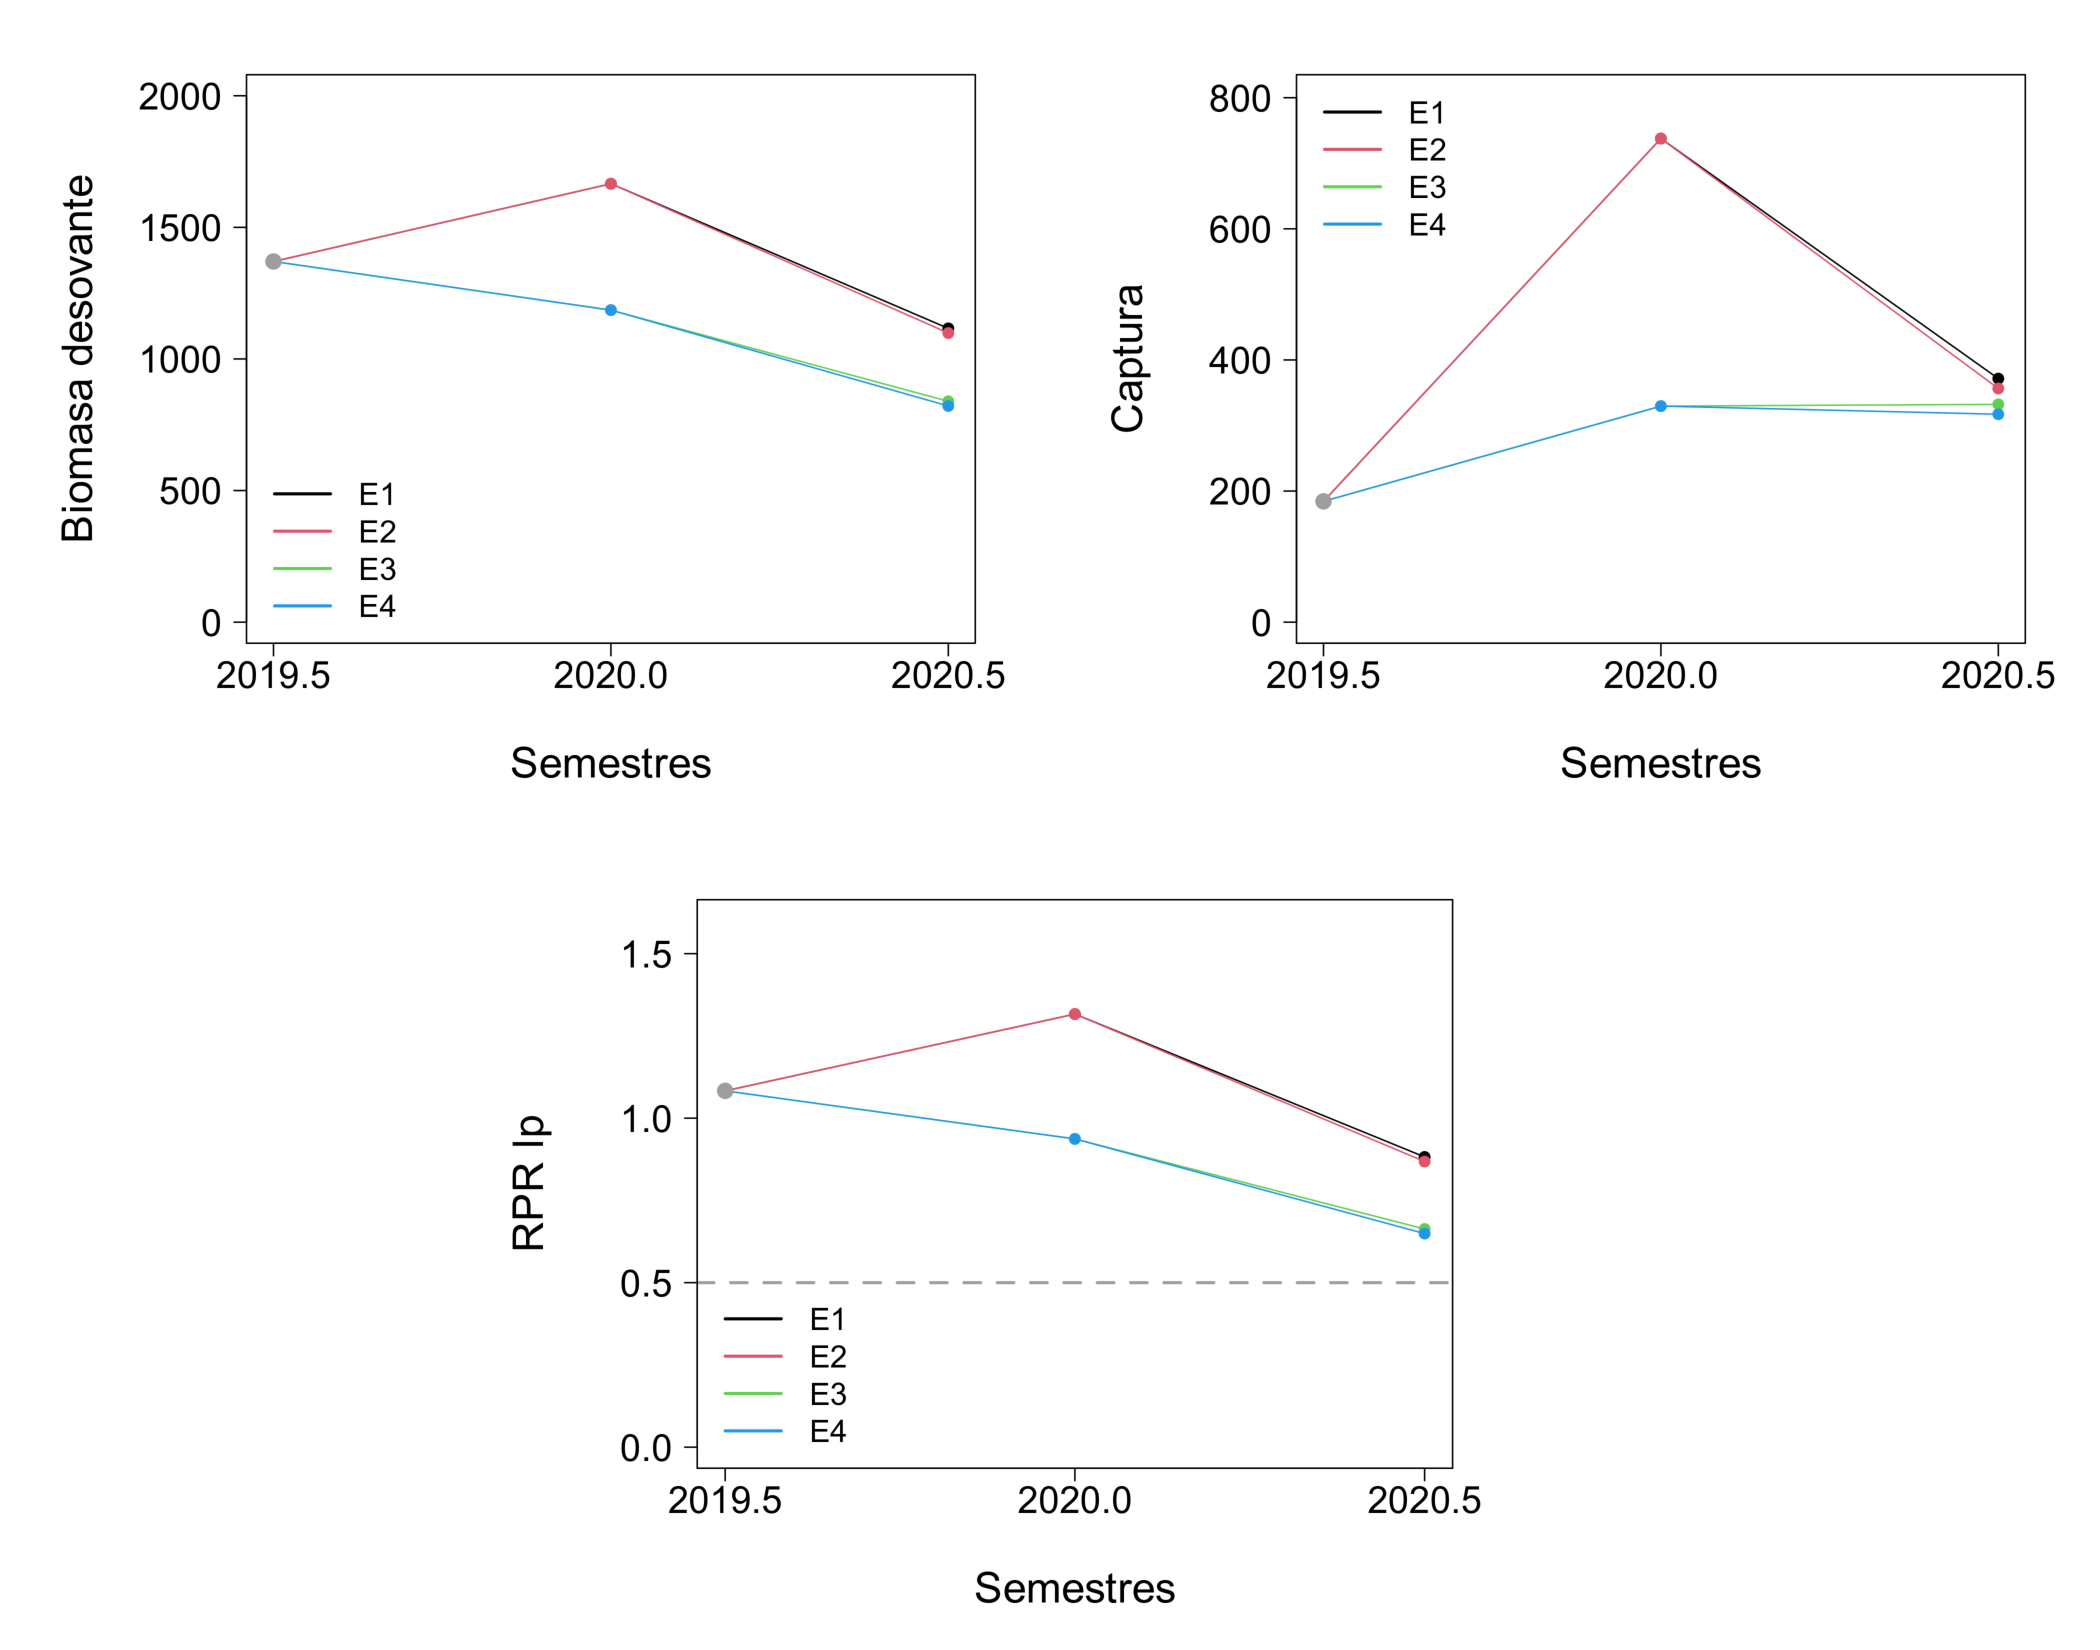
\includegraphics[width=13cm,height=11cm]{Figuras/figura22.pdf}
 \caption{Biomasa desovante (a), captura (b) y RPR largo plazao (c) proyectado para el segundo hito de asesor\'ia.}
 \label{Fig22}
\end{figure}


\vspace{0.5cm}
\begin{table}[htb!]
 \caption{CBA semestral proyectada (2020.0-2020.5) y anual para el 2020 para el stock de anchoveta dado el criterio del F=F$_{RMS}$ y los diferentes escenarios evaluados.}
 \label{Tab24}
 \centering
 \small
 \begin{tabular}{lccc}
 \hline\noalign{\vskip 0.1cm}
 Escenario & 2020.0 & 2020.5 & 2020$_{TOT}$ \\
 \hline\noalign{\vskip 0.1cm}
 E1  & 737.6 & 371.5 & 1109.2  \\
 E2  & 737.6 & 356.4 & 1094.0 \\
 E3  & 329.5 & 332.2 & 661.7 \\
 E4  & 329.5 & 317.1 & 646.6  \\
 \hline
 \end{tabular}
\end{table}


\subsubsection{Aporte de cada grupo de edad a la captura proyectada por semestre}

\quad

Durante la proyecci\'on del stock de anchoveta se estim\'o la captura en
n\'umero de individuos por grupo de edad (Baranov, 1918), y luego fue
dividida por la suma total de todos los grupos de edad. Este porcentaje
por grupo de edad en la captura es presentado en las
\textbf{Tabla \ref{Tab25}}, \textbf{Tabla \ref{Tab26}},
\textbf{Tabla \ref{Tab27}} y \textbf{Tabla \ref{Tab28}} para el
escenario E1, E2, E3 y E4, respectivamente. Independiente del escenario
evaluado, el grupo de edad 1 (6 meses) es que mayor porcentaje aporta a
la captura semestral. Para el escenario E1 y E2 este valor varia entre
un 89\% y un 80\%, y para el escenario E3 y E4 este valor varia entre un
75\% y un 84\%. En general, los grupos de edades 0 (reclutas), 1 (6
meses) y 2 (1 a\~{n}o) aportan el 100\% de la captural semestral para los
diferentes escenarios evaluados.\\

\vspace{0.5cm}
\begin{table}[htb!]
 \caption{Porcentaje por grupo de edad en la captura proyectada (2020) para el escenario E1.}
 \label{Tab25}
 \centering
 \small
 \begin{tabular}{lcc}
 \hline\noalign{\vskip 0.1cm}
 Edad & 2020.0 & 2020.5 \\
 \hline\noalign{\vskip 0.1cm}
 0 & 0.052 & 0.119  \\
 \rowcolor{Gray}
 1 & 0.894 & 0.804 \\
 2 & 0.051 & 0.073 \\
 3 & 0.001 & 0.002  \\
 \hline
 \rowcolor{Gray}
 Suma(0:2) & 0.998 & 0.997 \\
 \hline
 \end{tabular}
\end{table}


\vspace{0.5cm}
\begin{table}[htb!]
 \caption{Porcentaje por grupo de edad en la captura proyectada (2020) para el escenario E2.}
 \label{Tab26}
 \centering
 \small
 \begin{tabular}{lcc}
 \hline\noalign{\vskip 0.1cm}
 Edad & 2020.0 & 2020.5 \\
 \hline\noalign{\vskip 0.1cm}
 0 & 0.050 & 0.117  \\
 \rowcolor{Gray}
 1 & 0.896 & 0.802 \\
 2 & 0.051 & 0.076 \\
 3 & 0.001 & 0.002  \\
 \hline
 \rowcolor{Gray}
 Suma(0:2) & 0.998 & 0.997 \\
 \hline
 \end{tabular}
\end{table}


\vspace{0.5cm}
\begin{table}[htb!]
 \caption{Porcentaje por grupo de edad en la captura proyectada (2020) para el escenario E3.}
 \label{Tab27}
 \centering
 \small
 \begin{tabular}{lcc}
 \hline\noalign{\vskip 0.1cm}
 Edad & 2020.0 & 2020.5 \\
 \hline\noalign{\vskip 0.1cm}
 0 & 0.120 & 0.119  \\
 \rowcolor{Gray}
 1 & 0.759 & 0.849 \\
 2 & 0.117 & 0.028 \\
 3 & 0.002 & 0.002  \\
 \hline
 \rowcolor{Gray}
 Suma(0:2) & 0.997 & 0.997 \\
 \hline
 \end{tabular}
\end{table}


\vspace{0.5cm}
\begin{table}[htb!]
 \caption{Porcentaje por grupo de edad en la captura proyectada (2020) para el escenario E4.}
 \label{Tab28}
 \centering
 \small
 \begin{tabular}{lcc}
 \hline\noalign{\vskip 0.1cm}
 Edad & 2020.0 & 2020.5 \\
 \hline\noalign{\vskip 0.1cm}
 0 & 0.115 & 0.123  \\
 \rowcolor{Gray}
 1 & 0.763 & 0.843 \\
 2 & 0.118 & 0.080 \\
 3 & 0.002 & 0.002  \\
 \hline
 \rowcolor{Gray}
 Suma(0:2) & 0.997 & 0.997 \\
 \hline
 \end{tabular}
\end{table}


\subsubsection{Abundancia semestral proyectada}

\quad

En las \textbf{Tabla \ref{Tab29}}, \textbf{Tabla \ref{Tab30}},
\textbf{Tabla \ref{Tab31}} y \textbf{Tabla \ref{Tab32}} se presentan las
matrices de abundancia en n\'umero durante la proyecci\'on del stock de
anchoveta. En estas se observan los diferentes supuestos
(\textbf{Tabla \ref{Tab14}}) aplicados para cada uno de los casos
evaluados. Adem\'as, se muestra la abundancia por grupo de edad al \'ultimo
semestre estimado por el modelo de evaluaci\'on, de manera de identificar
el \'ultimo reclutamiento estimado (\textbf{Tabla \ref{Tab29}} y
\textbf{Tabla \ref{Tab30}}). Y en las \textbf{Tabla \ref{Tab31}} y
\textbf{Tabla \ref{Tab32}} se muestra el reclutamiento penalizado para
el semestre 2019.5.\\

\vspace{0.5cm}
\begin{table}[htb!]
 \caption{Abundancia semestral proyectada (2019.5 - 2020.5) para el escenario E1.}
 \label{Tab29}
 \centering
 \small
 \begin{tabular}{lrrr}
 \hline\noalign{\vskip 0.1cm}
 Edad & 2019.5 & 2020.0 & 2020.5 \\
 \hline\noalign{\vskip 0.1cm}
 0 & \cellcolor{Gray1}498.17 & \cellcolor{Gray2}239.04 & \cellcolor{Gray3}283.16 \\
 1 & 111.22 & \cellcolor{Gray1}165.00 & \cellcolor{Gray2}77.55 \\
 2 & 26.66 & 31.30 & \cellcolor{Gray1}23.24 \\
 3 & 8.57 & 8.52 & 8.49  \\
 4 & 1.89 & 2.84 & 2.79 \\
 5 & 0.48 & 0.79 & 1.21 \\
 \hline
 \end{tabular}
\end{table}

\vspace{0.5cm}
\begin{table}[htb!]
 \caption{Abundancia semestral proyectada (2019.5 - 2020.5) para el escenario E2.}
 \label{Tab30}
 \centering
 \small
 \begin{tabular}{lrrr}
 \hline\noalign{\vskip 0.1cm}
 Edad & 2019.5 & 2020.0 & 2020.5 \\
 \hline\noalign{\vskip 0.1cm}
 0 & \cellcolor{Gray1}498.17 & \cellcolor{Gray2}227.26 & \cellcolor{Gray3}265.29 \\
 1 & 111.22 & \cellcolor{Gray1}165.00 & \cellcolor{Gray2}73.73 \\
 2 & 26.66 & 31.30 & \cellcolor{Gray1}23.24 \\
 3 & 8.57 & 8.52 & 8.49  \\
 4 & 1.89 & 2.84 & 2.79 \\
 5 & 0.48 & 0.79 & 1.21 \\
 \hline
 \end{tabular}
\end{table}


\vspace{0.5cm}
\begin{table}[htb!]
 \caption{Abundancia semestral proyectada (2019.5 - 2020.5) para el escenario E3.}
 \label{Tab31}
 \centering
 \small
 \begin{tabular}{lrrr}
 \hline\noalign{\vskip 0.1cm}
 Edad & 2019.5 & 2020.0 & 2020.5 \\
 \hline\noalign{\vskip 0.1cm}
 0 & \cellcolor{Gray1}185.15 & \cellcolor{Gray2}239.04 & \cellcolor{Gray3}267.53 \\
 1 & 111.22 & \cellcolor{Gray1}61.44 & \cellcolor{Gray2}77.55 \\
 2 & 26.66 & 31.30 & \cellcolor{Gray1}8.65 \\
 3 & 8.57 & 8.52 & 8.49  \\
 4 & 1.89 & 2.84 & 2.79 \\
 5 & 0.48 & 0.79 & 1.21 \\
 \hline
 \end{tabular}
\end{table}


\vspace{0.5cm}
\begin{table}[htb!]
 \caption{Abundancia semestral proyectada (2019.5 - 2020.5) para el escenario E4.}
 \label{Tab32}
 \centering
 \small
 \begin{tabular}{lrrr}
 \hline\noalign{\vskip 0.1cm}
 Edad & 2019.5 & 2020.0 & 2020.5 \\
 \hline\noalign{\vskip 0.1cm}
 0 & \cellcolor{Gray1}185.15 & \cellcolor{Gray2}227.26 & \cellcolor{Gray3}265.29 \\
 1 & 111.22 & \cellcolor{Gray1}61.44 & \cellcolor{Gray2}73.73 \\
 2 & 26.66 & 31.30 & \cellcolor{Gray1}8.65 \\
 3 & 8.57 & 8.52 & 8.49  \\
 4 & 1.89 & 2.84 & 2.79 \\
 5 & 0.48 & 0.79 & 1.21 \\
 \hline
 \end{tabular}
\end{table}




\clearpage
\newpage

\section{REFERENCIAS BIBLIOGR\'AFICAS}

\quad

Basilone, G., C. Guisande, B. Patti, S. Mazzola, A. Cuttitta, A.
Bonanno, A.R. Vergara y I. Maneiro. 2006. Effect of habitat condictions
on reproduction of the European anchovy
(\textit{Engraulis encrasicolus}) in the Strait of Sicily.
\textit{Fish. Ocenaogr.}, 15:4, 271-280.

Bertrand, A., M. Segura, M. Guiti\'errez y L. V\'asquez. 2004. From
small-scale habitat loopholes to decadal cycles: a habitat-based
hypothesis explaining fluctuation in pelagic fish populations off Peru.
\textit{Fish Fish.}, 5: 296-316.

Baranov, F.I. 1918. On the question of the biological basis of
fisheries,
\textit{Nauchnye Issledovaniya Ikhtiologicheskii Instituta Izvestiya},
vol.~1, 81-128 pp.

Beverton, R.J.H. y S.J. Holt. 1957. On the dynamics of exploited fish
populations. \textit{Fish. Invest. Ser.} 2, 19, 533 pp.

Blanco, J.L., A.C. Thomas, M.E. Carr y P.T. Strub. 2001. Seasonal
climatology of hydrographic conditions in the upwelling region off
northern Chile. \textit{J. Geophys. Res.}, 106, 11,451-11,467.

B\"ohm, G., C. Hern\'andez, G. P\'erez, E. D\'iaz, L. Cortez, L. Ossa, F. Cerna,
C. Valero, C. Machuca, L. Mu\~{n}oz, H. Reyes, M. Troncoso, C. Gaspar, Z.
Young y R. Aravena. 2013. Asesor\'ia integral para la toma de decisiones
en pesca y acuicultura, 2013. Actividad 1: Recursos pel\'agicos: Pesquer\'ia
Recursos pel\'agicos Zona Norte. Subsecretaria de Econom\'ia. Informe Final.
267 pp.

B\"ohm, G., C. Hern\'andez, E. D\'iaz, R. Ojeda, F. Cerna, C. Valero, C.
Machuca, L. Mu\~{n}oz, C. Rozas, H. Reyes, M. Pizarro, R. Aravena, M.
Troncoso, C. Gaspar y Z. Young. 2016. Programa de Seguimiento de las
Pesquer\'ias Pel\'agicas Zona Norte. Subsecretaria de Econom\'ia y EMT.
Informe Final. 364 pp.

Bowler, D.E. et. al.~2017. Cross-realm assessment of climate change
impacts on species abundance trends. \textit{Nat. Ecol.} Evol. 1, 0067.

Butler, J. 1989. Growth during the larval and juveniles stages of the
northern anchovy \textit{Engraulis mordax} in the California Current,
1980-1984. \textit{Fish. Bull}. 87: 645-652.

Cai, W., S. Borlace, M. Lengaigne, P. van Rensch, M. Collins, G. Vecchi,
A. Timmermann, A. Santoso, M.J. McPhaden, L. Wu, M.H. England, G. Wang,
E. Guilyardi y F.F. Jin. 2014. Increasing frequency of extreme El Ni\~{n}o
events due to greenhouse warming. \textit{Nature Clim. Change}, 4:
111-116.

Canales, T. M. y E. Leal. 2009. Par\'ametros de historia de vida de la
anchoveta \textit{Engraulis ringens Jenyns}, 1842, distribuida en la
zona centro norte de Chile. \textit{Rev. Biol. Mar. Oceanogr.}, 44(1):
173-179.

Canales, C., R. Wiff y J.C. Quiroz. 2011. Estatus y posibilidades de
explotaci\'on biol\'ogicamente sustentables de los principales recursos
pesqueros nacionales, a\~{n}o 2012. Metas Cualitativas; Cuarto Objetivo
Espec\'ifico. Informe Final. 23 pp+Anexos.

Canales, T.M. C. Canales, M.G. B\"ohm y C. Castillo. 2014. Estatus y
posibilidades de explotaci\'on biol\'ogicamente sustentables de los
principales recursos pesqueros nacionales, a\~{n}o 2014. Proyecto 2.6.
Investigaci\'on del status y posibilidades de explotaci\'on biol\'ogicamente
sustentables de anchoveta y sardina espa\~{n}ola regiones XV a II, a\~{n}o 2014:
Anchoveta XV - II Regiones, 2014. Informe Final. Instituto de Fomento
Pesquero. 39 pp.+ Anexos.

Carmichael, J. y K. Fenske. 2010. Third National Meeting of the Regional
Fisheries Management Councils`s Scientific and Statistical Committees.
Report of a National SSC Workshop on BC Control Rule Implementation and
Peer Review Procedures. 95 pp.

Castillo, J. A. Saavedra, C. Hern\'andez, V. Catasti, F. Leiva, J.
Letelier, H. Reyes, M. Pizarro, B. Leiva, F. Cerna, A. L\'opez, L.
Herrera, G. Claramunt, A. Mujica y E. Uribe. 2009. Evaluaci\'on
hidroac\'ustica reclutamiento anchoveta entre la XV y IV Regiones, a\~{n}o
2009. Informe Final. FIP 2008-02. 285 pp + Figuras, Tablas y Anexos.

Castillo, J. A. Saavedra, F. Leiva, H. Reyes, M. Pizarro, F. Esp\'indola,
V. Catasti, C. Lang, C. Hern\'andez, B. Leiva, F. Cerna, A. L\'opez, L.
Herrera, G. Claramunt, E. Oliva, P. Moreno y M. Medina. 2010. Evaluaci\'on
hidroac\'ustica del reclutamiento de anchoveta en la XV, I y II Regiones,
a\~{n}o 2010. Informe Final. FIP 2009-02. 225 pp + Figuras, Tablas y Anexos.

Castillo, J. A. Saavedra, F. Leiva, H. Reyes, M. Pizarro, V. Catasti, C.
Lang, M., San Martin, B. Leiva, F. Cerna, A. L\'opez y L. Herrera. 2011.
Evaluaci\'on hidroac\'ustica del reclutamiento de anchoveta en la XV, I y II
Regiones, a\~{n}o 2011. Informe Final. FIP 2010-13. 248 pp + Figuras, Tablas
y Anexos.

Castillo, J. A. Saavedra, F. Leiva, H. Reyes, M. Pizarro, V. Catasti, C.
Lang, M., San Martin, B. Leiva, F. Cerna, A. L\'opez y L. Herrera. 2012.
Evaluaci\'on hidroac\'ustica del reclutamiento de anchoveta en la XV, I y II
Regiones, a\~{n}o 2012. Informe Final. FIP 2010-13. 248 pp + Figuras, Tablas
y Anexos.

Castillo, J. A. Saavedra, F. Leiva, H. Reyes, M. Pizarro, V. Catasti, C.
Lang, M., San Martin, B. Leiva, F. Cerna, A. L\'opez y L. Herrera. 2013.
Evaluaci\'on hidroac\'ustica del reclutamiento de anchoveta en la XV, I y II
Regiones, a\~{n}o 2013. Pre-Informe Final. FIP 2012-11. 248 pp + Figuras,
Tablas y Anexos.

Cerna, F. y G. Plaza. 2016. Daily growth patterns of juveniles and
adults of the Peruvian anchovy (Engraulis ringens) in northern Chile.
\textit{Mar. Fresh. Res.}, \href{http://dx.doi.org/10.1071/MF15032}.

Chirichigno, N. y J. V\'elez. 1998. Clave para identificar los peces
marinos del Per\'u (2$^{da}$ edici\'on). Pub. Esp. Inst. Mar Per\'u. 500 p.~

CIAM, 2017. Condici\'on biol\'ogica pesquera y ambiental de las regiones XV,
I y II. Informe mensual -- Marzo del 2017. 38 pp.

Claramunt, G., L.R. Castro, L.A. Cubillos, Hans-Jurgen Hirche, G. Perez
y M. Braun. 2012. Inter-annual reproductive trait variation and spawning
habitat preferences of \textit{Engraulis ringens} off northern Chile.
\textit{Rev. Biol. Mar. Oceanogr.}, 47(2): 227-243.

Claramunt, G., Herrera, G., Moreno, P. y Azocar, C. 2014. Evaluaci\'on de
la biomasa desovante de anchoveta en la XV, I y II Regiones, A\~{n}o 2013.
Pre-Informe Final. FIP 2013-06.

Contreras-Reyes, J.E., T.M. Canales y P.M. Rojas. 2016. Influence of
climate variability on anchovy reproductive timing off northern Chile.
\textit{J. Mar. Sys.}, 164: 67-75.

Correa-Ram\'irez, M., S. Hormazabal y G. Yuras. 2007. Mesoscale eddies and
high chlorophyll concentrations off central Chile.
\textit{Geophys.  Res. Lett.}, 34, L12604,
\url{doi:10.1029/2007GL029541}.

Correa-Ram\'irez, M.A., S.E. Hormazabal y C.E. Morales. 2012. Spatial
patterns of annual and interannual surface chlorophyll-a variability in
the Peru-Chile Current System. \textit{Prog. Oceanogr.}, 92-95: 8-17.

Cubillos, L. A., R. Serra y P. Fr\'eon. 2007. Synchronous pattern of
fluctuation in three anchovy fisheries in the Humboldt Current System.
\textit{Aquat. Living Resour.}, 75:69--75.

Esp\'indola, F. y J.C. Quiroz. 2017. Estatus y posibilidades de
explotaci\'on biol\'ogicamente sustentables de los principales recursos
pesqueros nacionales, a\~{n}o 2018, Anchoveta XV - II Regiones, 2017.
Informe 1 Estatus. IFOP. 131 pp.

FAO (1997) Enfoque Precautorio para la Pesca de Captura y la
Introducci\'on de especies. FAO Orientaciones T\'ecnicas para la Pesca
Responsable. N°2. Roma. FAO. 64 p.

FAO (2003) La ordenaci\'on pesquera. El enfoque de ecosistemas en la
pesca. FAO Orientaciones t\'ecnicas para la pesca responsable. No.~4,
Supl. 2. Roma, FAO, 133 pp.~

Gavaris, S. y J.N. Ianelli. 2002. Statistical issues in fisheries stock
assessments. \textit{Scand. J. Statist.}, 29: 245-267.

Gruus, A., W.J. Harford, M.J. Schirripa, L. Velez, S.R. Sagarese, Y.
Shin y P. Verley. 2016. Management strategy evaluation using the
individual-based, multispecies modeling approach OSMOSE.
\textit{Ecol. Model.}, 340: 86-105.

Hansen, J., M. Soto, R. Ruedy, K. Lo, D.W. Lea y M. Medina-Elizade.
2006. Global temperature change. \textit{Proc. Nat. Acad. Sci.} USA
103(39): 14288-14293.

Hormazabal, S., G. Shaffer, J. Letelier y O. Ulloa. 2001. Local and
remote forcing of sea surface temperature in the coastal upwelling
system off Chile. \textit{J. Geophys. Res.}, 106, 16,657-16,671.

Leal E. y C. Canales. 2014. Convenio de Desempe\~{n}o: Estatus y
posibilidades de explotaci\'on biol\'ogicamente sustentables de los
principales recursos pesqueros nacionales, 2015. Anchoveta III-IV
Regiones. Informe de estatus y cuota. 110 pp.

Leiva, F., R. Vargas, C. Grendi, U. Cifuentes, C. Rozas, B. Leiva, F.
Cerna, A. L\'opez, C. Lang, L. Herrera, J. Jaque, J. Angulo y V.
Valenzuela. 2016. Evaluaci\'on hidroac\'ustica del reclutamiento de
anchoveta en la XV, I y II Regiones, a\~{n}o 2015. Informe Final, IFOP, 335
pp.

Leiva, F., B. Leiva, F. S\'anchez, M. Pizarro, C. Grendi, A. Bustamante,
U. Cifuentes. 2018. Evaluaci\'on hidroac\'ustica del reclutamiento de
anchoveta en la XV, I y II Regiones, a\~{n}o 2017. Informe de Avance, IFOP,
87 pp.

Longhurst, A.R., S. Sathyendranath, T. Platt y C. Cavehill. 1995. An
estimate of global primary production in the ocean from satellite
radiometer data. \textit{J. Plankton Res.} 17, 1245-1271.

Mart\'inez, C., Baros., V., Cortes., M et al.~1998. Programa de Marcaje de
Anchoveta. Fase I: Marcacio. Informe Final FIP-IT/96-04. Fondo de
Investigaci\'on Pesquera (FIP), 88 pp +Anexos.

Mart\'inez, C., G. B\"ohm, E. D\'iaz, L. Ossa, H. Reyes, R. Aravena, F. Cerna,
V. Boic, C. Machuca, L. Mu\~{n}oz y M. Troncoso. 2009. Programa: Seguimiento
del Estado de Situaci\'on de las Principales Pesquer\'ias Nacionales.
Proyecto: Investigaci\'on de la Situaci\'on de la Pesquer\'ia Pel\'agica de la
Zona Norte, 2008 -- Informe Final. Convenio SUBPESCA -- IFOP. Instituto
Fomento Pesquero, Valpara\'iso, Chile.

Medina, M., L. Herrera, J. Castillo, J. Jaque y N. Pizarro. 2015.
Alimentaci\'on de la anchoveta (Engraulis ringens) en el norte de Chile
(18\degree 25\texttt{-25\textbackslash{}degree\ 40}S) en diciembre de
2010. \textit{Lat. Am. J. Aquat. Res.}, 43(1): 46-58.

Melo, Y. C. 1984. Age studies on anchovy \textit{Engraulis capensis}
Gilchrist off South West Africa. \textit{S. Afr. J. Mar. Sci.} 2: 19-31.

Niklitschek, E., C. Garc\'es y P. Toledo. 2017. Determinaci\'on de unidades
poblacionales de anchoveta (\textit{Engraulis ringens}) en Chile. Informe
Pre-Final. Universidad de Los Lagos. 186 pp.

\~{N}iquen, M. y M. Bouchon. 2004. Impact of El Ni\~{n}o events on pelagic
fisheries in Peruvian waters. \textit{Deep-Sea Res. II}, 51, 563-574.

NRC-National Research Council. 1998. Improving Fish Stock Assessments.
National Academic Press. Washington D.C.: 188 pp.

Pay\'a I, C. Canales, D. Bucarey, M. Canales, F. Contreras, F. Esp\'indola,
E. Leal, R. Tascheri, A. Ya\~{n}ez y M.J. Z\'u\~{n}iga. 2014. Proyecto 2.16:
Revisi\'on de los puntos biol\'ogicos de referencia (Rendimiento M\'aximo
Sostenible) en las pesquer\'ias nacionales. Convenio II: Estatus y
posibilidades de explotaci\'on biol\'ogicamente sustentables de los
principales recursos pesqueros nacionales a\~{n}o 2014. Informe Final.
Subsecretaria de Econom\'ia y EMT - IFOP. 51 pp.+ 4 Anexos.

Pinheiro, J.C. y D.M. Bates. 2000. Mixed-Effects Models in S and S-PLUS.
Spinger-Verlag, New York, 528 pp.

Plaza, G., F. Cerna y J. Legua. 2012. Validaci\'on de formaci\'on de anillos
primarios y macro-anillos de crecimiento en otolitos de anchoveta de la
zona norte. Informe Final. PROY. SUBPESCA ID Nº4728-31LP11. 130 pp.

Plaza, G., M. Landaeta, A. Hern\'andez, J. Contreras, C. Rodr\'iguez, J.
Merino, D. Queirolo, F. Cerna, M. G\'omez, C. Machuca y F. Esp\'indola.
2017. Revisi\'on experta de la estimaci\'on y asignaci\'on de edad de la
anchoveta XV-II Regi\'on. Informe Final. Proyecto FIP 2014-31. 125 pp.

Prosch, R. M. 1986. Early growth in length of the anchovy
\textit{Engraulis capensis} Gilchrist off South Africa.
\textit{S. Afr. J. Mar. Sci.} 4: 181-191.

Restrepo V.R., G.G. Thompson, P.M. Mace, W.L. Gabriel, L.L. Low, A.D.
MacCall, R.D. Methot, J.E. Powers, B.L. Taylor, P.R. Wade, y J.F.
Witzig. 1998. Technical Guidance On the Use of Precautionary Approaches
to Implementing National Standard 1 of the Magnuson-Stevens Fishery
Conservation and Management Act. NOAA Technical Memorandum NMFS-F/SPO.

Rojas O, A Mujica, M Labra, G Lederman y H Miles. 1983. Estimaci\'on de la
abundancia relativa de huevos y larvas de peces. Informe IFOP/CORFO
83-31: 1-99.

Saetersdal, G. y J.E. Valdivia. 1964. Un estudio del crecimiento, tama\~{n}o
y reclutamiento de la anchoveta (\textit{Engraulis ringens J.}) basado en datos
de frecuencia de longitud. Instituto de Investigaci\'on de los Recursos
Marinos, La Punta, Callao, Per\'u. Boletin Nº 4, vol 1, 85-136 pp.

Schnute, J. y Fournier, D. 1980. A new approach to length-frequency
analysis: Growth Structure. \textit{Can. J. Fish. Aquat. Sci.}, 37(9):
1337-1351.

Serra, R. y E. Gil. 1975. Marcaci\'on de anchoveta en la zona norte de
Chile. Metodolog\'ia y trabajos preliminares.
\textit{Rev. Com. Perm. Pacifico Sur}, 3: 3-19.

Serra, J.R. 1983. Changes in the abundance of pelagic resources along
the Chilean coast. \textit{In:} G.D. Sharp and J. Csirke (Eds.)
Proceedings of the Expert Consultation to examine changes in abundance
and species composition of neritic fish resources. San Jos\'e, Costa Rica,
18 - 29 April 1983. \textit{FAO Fish. Rep.} 291 (2): 255 - 284.

Serra, R. y C. Canales. 2011. Investigaci\'on del Estatus y Evaluaci\'on de
Estrategias de Explotaci\'on Sustentables 2011, de las Principales
Pesquer\'ias Chilenas. Actividad 1: Peces Pel\'agicos: Anchoveta y sardina
espa\~{n}ola XV, I y II Regiones. 2011.

Serra, R. y C. Canales. 2012. Estatus y Posibilidades de Explotaci\'on
Biol\'ogicamente Sustentables de los Principales Recursos Pesqueros
Nacionales, A\~{n}o 2012. Evaluaci\'on de Estrategias de Explotaci\'on
Sustentables 2011, de las Principales Pesquer\'ias Chilenas. Actividad 1:
Peces Pel\'agicos: Anchoveta y sardina espa\~{n}ola XV, I y II Regiones. 2011.

Serra, R. y C. Canales. 2013. Investigaci\'on del Estatus y Evaluaci\'on de
Estrategias de Explotaci\'on Sustentables 2013, de las Principales
Pesquer\'ias Chilenas. Actividad 1: Peces Pel\'agicos: Anchoveta y sardina
espa\~{n}ola XV, I y II Regiones. 2011. Informe Final.

Silva, C., M.A.Barbieri, E. Y\'a\~{n}ez, J.C. Guiti\'errez-Estrada y T.M.
DelValls. 2012. Using indicators and models for an ecosystem approach to
fisheries and aquaculture management: the anchovy fishery and Pacific
oyster culture in Chile: case studies. \textit{Lat. Am. J. Aquat. Res.},
40(4): 955-969.

Simpson, J. y R. Buzeta. 1967. El crecimiento y la edad de la anchoveta
(\textit{Engraulis ringens, Jenyns}) en Chile basado en estudios de
frecuencia de longitud. \textit{Bolet\'in Cient\'ifico}, Nº 3. IFOP. 56 pp.

Ya\~{n}ez-Rubio, A., A. Llanos-Rivera, L. Castro, G. Claramunt y L. Herrera.
2011. Variations in type, width, volume and carbon content of anchoveta,
Engraulis ringens food items during the early larval stages.
\textit{J. Mar. Biol. Assoc. U. K.}, 91(6): 1207-1213.

Y\'a\~{n}ez, E., A. Gonz\'alez y M.A. Barbieri. 1995. Estructura t\'ermica
superficial del mar asociada a la distribuci\'on espacio-temporal de
sardina y anchoveta en la zona norte de Chile entre 1987 y 1992.
\textit{Invest. Mar.}, 23:123-147.

Valle-Levinson A y J Moraga-Opazo. 2006. Observations of bipolar
residual circulation in two equatorward-facig semiarid bays.
\textit{Cont. Shelf Res.}, 26: 179-193.

Vega R., L. Ossa, B. Su\'arez, M.F. Jim\'enez, S. Henr\'iquez, A. Gonz\'alez, R. Ojeda, A.
Simeone, C. Anguita, M. Sep\'ulveda, M.J. P\'erez, M. Santos, J. Cavieres, P. Paredes,
I. Cari, P. Z\'arate y D. Devia. 2020. INFORME FINAL. Programa de
observadores cient\'ificos: Programa de investigaci\'on y monitoreo del
descarte y de la captura de pesca incidental en pesquer\'ias pel\'agicas,
2019-2020. Subsecretaria de Econom\'ia y EMT. Instituto de Fomento Pesquero
(IFOP), Valpara\'iso, Chile. 341 p + Anexos.

Waldron, M., M.J. Armstrong y R.M. Prosch. 1989. Aspects of the
variability in growth of juvenile anchovy \textit{Engraulis capensis} in
the southern Benguela System. \textit{S. Afr. J. Mar. Sci.}, 8:9-19.

Waldron, M., M.J. Armstrong y B.A. Roel. 1992. Birthdate distribution of
juvenile anchovy \textit{Engraulis capensis} caught in the southern
Benguela System. \textit{S. Afr. J. Mar. Sci.}, 12: 865-871.


\newpage
\pagestyle{empty}
\begin{tikzpicture}
\node[anchor=south west,inner sep=0] at (0,0) {
\includegraphics[height=22.3cm,width=22cm,viewport=70 74 318 698]{portada3.pdf}};
\end{tikzpicture}


\newpage
\begin{tikzpicture}
\node[anchor=south west,inner sep=0] at (0,0) {
\includegraphics[height=22.3cm,width=22cm,viewport=29 26 148 274]{portada4.pdf}};
%\node[anchor=south west,inner sep=0] at (0,0) {
\includegraphics[height=22.3cm,width=22cm,viewport=70 74 318 698]{portada4.pdf}};
\end{tikzpicture}




\end{document}
